% Created 2019-10-24 Thu 09:26
% Intended LaTeX compiler: pdflatex
\documentclass[11pt]{book}
\usepackage[utf8]{inputenc}
\usepackage[T1]{fontenc}
\usepackage{graphicx}
\usepackage{grffile}
\usepackage{longtable}
\usepackage{wrapfig}
\usepackage{rotating}
\usepackage[normalem]{ulem}
\usepackage{amsmath}
\usepackage{textcomp}
\usepackage{amssymb}
\usepackage{capt-of}
\usepackage{hyperref}
\usepackage{minted}
\usepackage[margin=1in] {geometry}
\usepackage{parskip}
\setlength\parindent{0pt}
\linespread {1.0}
\setcounter{tocdepth} {6}
\setcounter{secnumdepth} {6}
\usepackage{fontspec}
\usepackage{fancyvrb}
\setmonofont{Droid Sans Mono}[SizeFeatures={Size=9}]
\date{\today}
\title{}
\hypersetup{
 pdfauthor={},
 pdftitle={},
 pdfkeywords={},
 pdfsubject={},
 pdfcreator={Emacs 26.2 (Org mode 9.2.3)}, 
 pdflang={English}}
\begin{document}

\tableofcontents


\part{C++ Generals}
\label{sec:orgfeb6c32}
Most of C++ generals content are from my \emph{Starting out with C++} notes. 

\chapter{Expressions and Interactivity}
\label{sec:org106d664}

\section{cin object and stream extraction operator}
\label{sec:org825d668}
\begin{minted}[linenos,firstnumber=1,breaklines=true,breakanywhere=true,frame=single,framesep=10pt]{c++}
cin >> a;
\end{minted}

\chapter{Inheritance, Polymorphism and Virtual Functions}
\label{sec:org11548ce}
\section{Inheritance}
\label{sec:org3e2c37e}
\subsection{Concept}
\label{sec:orga43abd6}
\begin{itemize}
\item Inheritance allows a new class to be based on an existing class;
\item The new class inherits all the member variables and functions of the class it based on
\item The new class won't inherit constructors and destructor of the class it based on
\end{itemize}

\subsection{Origin of Inheritance: Generalization and Specialization}
\label{sec:org73812aa}
In the real world you can find many objects that are specialized versions of other more general objects. For example, dog is a specialized object of animal.

Inheritance allows abstraction of this kind of relation: creating new class that is based on an existing class. When one object is a specialized version of another object, there is an ``is a'' relationship between them, for example: a tree is a plant, a dog is an animal.

When an ``is a'' relationship exists between classes, it means that the specialized class has all of the characteristics of the general class, plus additional characteristics that make it special. In object-oriented programming, inheritance is used to create an ``is a'' relationship between classes. 

Inheritance involves a base class and a derived class. The base class is the general class and the derived class is the specialized class. The derived class has following features:
\begin{itemize}
\item it inherits the member variables and member functions of the base class without any of them being rewritten (including private and public members)
\item it does not inherit constructors and destructor
\item it can be added with new member variables and functions, making it more specialized than the base class
\end{itemize}

\subsection{Syntax}
\label{sec:orge1739a4}
Suppose you have a \texttt{Base} class. Now you want to make a derived class from \texttt{Base} named \texttt{Derived}. You declare the \texttt{Derived} class in following way:
\begin{minted}[linenos,firstnumber=1,breaklines=true,breakanywhere=true,frame=single,framesep=10pt]{c++}
class Derived : public Base {
  // class definition
  // goes here
};
\end{minted}

This declaration tells you that, \texttt{Derived} is a \texttt{Base}. Similarly, we can have:
\begin{minted}[linenos,firstnumber=1,breaklines=true,breakanywhere=true,frame=single,framesep=10pt]{c++}
class Dog : public Animal; // Dog is an Animal
class Tree : public Plant; // Tree is a plant
class Ginkgo : public Tree; // Ginko is a Tree
\end{minted}

You have to \texttt{\#include} the base class header file in the derived class's header file.

The word, public which precedes the name of the Base class, is the base class access specification. It affects how the members of the Base class are inherited by the Derived class. When you create an object of a Derived class, you can think of it as being built on top of an object of the Base class. The members of the Base class object becomes members of the Derived class object automatically. How the Base class members appear in the Derived class is determined by the base class access specification. Base class access specification will be covered in detail in next section (Class Access).

If you declare the base class access specification as public, you can access the public members of the Base class without any additional declarations. For example, you can call  public member functions of the Base class. Although you can't access the private member of the Base class directly in the Derived class, you can access them via the interface defined in public of the Base class.

Inheritance does not work in reverse. It is not possible for a base class to call a member function of a derived class.

\subsection{Class Access Specifications}
\label{sec:orga1c78a1}
There are three class access specifications between a base class and a derived class:
\begin{minted}[linenos,firstnumber=1,breaklines=true,breakanywhere=true,frame=single,framesep=10pt]{c++}
class Derived : private Base;
class Derived : protected Base;
class Derived : public Base;
\end{minted}

\emph{Details omitted}

\subsection{Constructors and Destructors in Base and Derived Classes}
\label{sec:org28ae43e}
\subsubsection{Calling order}
\label{sec:org2bb215f}
Suppose you have a Derived class and a Base class. Now you are defining an object of a Derived class. Then you exit the program so the Derived object is destroyed. The order of calling constructors and destructor is as follows:
\begin{itemize}
\item constructor of base class
\item constructor of derived class
\item destructor of derived class
\item destructor of base class
\end{itemize}

\subsubsection{Passing arguments to base class constructors}
\label{sec:orgebf992f}
Consider following case:
\begin{minted}[linenos,firstnumber=1,breaklines=true,breakanywhere=true,frame=single,framesep=10pt]{c++}
class Derived : public Base
\end{minted}

When you are creating a Derived object, you will first call the constructor of Base class. In order to pass arguments to Base class constructor, you have to let the Derived class constructor pass arguments to the Base class constructor.

Now, suppose the Base class has a constructor that needs two arguments: length and width. And Derived class has a constructor that needs one argument: height. When you write the parameter list for constructor of Derived class, you can also include the parameter for constructor of Base class. Here is how you should write when you \textbf{implement the constructor}.
\begin{minted}[linenos,firstnumber=1,breaklines=true,breakanywhere=true,frame=single,framesep=10pt]{c++}
Derived::Derived() : Base() {
  // implementation of default constructor 
}

Derived::Derived(double len, double w, double h) : Base(len, w) {
  // implementation of Derived(len, w, h)
}
\end{minted}

Pay attention that, calling and passing parameter to \texttt{Base()} is when you \textbf{IMPLEMENT} \texttt{Derived} class's constructor. When declaring constructor of \texttt{Derived} class, you write in the normal way:
\begin{minted}[linenos,firstnumber=1,breaklines=true,breakanywhere=true,frame=single,framesep=10pt]{c++}
Derived();
Derived(double len, double w, double h);
\end{minted}
however, if you are writting the constructor inline, you have to write it in .h file.

\textbf{Note 1} 
The order of the parameter in Derived class constructor is not required. You just need to put the argument in the followed Base class constructor in right order.

\textbf{Note 2} 
The Base class constructor is always executed before the Derived class constructor. It will take the argument it needs in the argument list of Derived class constructor, and executes. When the Base constructor finishes, the Derived class constructor is then executed.

\textbf{Note 3}
If the Base class has no default constructor, then the Derived class must have a constructor that calls one of the Base class constructors. Because normally, if all the Derived class constructor don't call Base class constructor, when a Derived  class object is made, the default Base class constructor will be called.

\subsubsection{Redefining \texttt{Base} class functions}
\label{sec:orga803a46}
You can redefine a Base class member function in its Derived  class. Its like an overloaded member function (because the function has the same name), however, there is a distinction between redefining a function and overloading a function:
\begin{itemize}
\item Overloading functions must have \textbf{DIFFERENT} function signature (same function name, but different parameter list)
\item Redefining function must have \textbf{SAME} function signature. Redefining happens when a Derived class has a function with the same name and same parameter list as a Base class function.
\end{itemize}

Suppose you have following classes defined:
\begin{minted}[breaklines=true,breakanywhere=true,frame=single,framesep=10pt]{c++}
class Derived : public Base
\end{minted}

There is a function \texttt{func(int num)} in Base class. Now you want to redefine \texttt{func()} in Derived class. You can directly declare it in header file of Derived class:
\begin{minted}[linenos,firstnumber=1,breaklines=true,breakanywhere=true,frame=single,framesep=10pt]{c++}
class Derived : public Base {
private:
  // declaration of private member
public:
  void func(int num2) { // define the func() directly

    int num = num2 / 2;
    Base::func(num); // you can call the original func() in Base using scope resolution operator 

    // additional definition
    // goes here
  }
};
\end{minted}

If you redefine the function. You have to use the scope resolution operator :: to call the original function in Base class. C++ cast static binding to re-defined member function. That is, function call and the corresponding function is bound together when compiling.

\part{Data Structures}
\label{sec:orgc859dee}
\chapter{Vector}
\label{sec:org94c793b}
\chapter{List}
\label{sec:orgeaecb39}
Some portion of this section is copied from my \emph{Starting out with C++} notes. The implementation is from my project 2 of COP 4530 course.
\section{General Idea}
\label{sec:org57f545f}
Suppose you design a program that will dynamically allocate data structures, and you want to manage them. You can use linked list to do this job.

Dynamically allocated data structures may be linked together in memory to form a chain (linked list), each dynamically allocated data structure in that linked list is called \textbf{node}. A linked list can easily grow or shrink in size. Also, compared with vector, it is very efficient for a linked list to insert an element into the middle of the list, or delete an element that is in the middle. For a vector, to access a middle element you have to move all the element after that position, while for a linked list, none of the other nodes have to be moved.

A linked list is a series of connected nodes, where each node is a data structure. By saying ``connected'', it means that there is a pointer in each node that points to next node, thus the term ``connected''. Data members hold the data that this node contain (one or more members). In addition to the data, each node contains a pointer, which can point to another node (the next node). A linked list is formed when each node points to the next node. A \textbf{doubly linked list} is when each node contains two pointers, which can link to the previous node and the next node.
\section{Simple Implementation}
\label{sec:org4ce7888}
In this section, we'll implemente a doubly linked list, which has similar interface as the STL list. We'll also implement a nested iterator class in the list.
\subsection{Outline of List Class}
\label{sec:org7b4e22f}
We'll encapsulate three types in \texttt{List} class: 1. the node structure; 2. the nested constant iterator; 3. the nested iterator. Our \texttt{List} class will also support similar interface with STL list. Aside from member functions, our \texttt{List} class has the following data members:
\begin{minted}[breaklines=true,breakanywhere=true,frame=single,framesep=10pt]{c++}
int theSize; // number of elements in the list
Node* head; // store head node
Node* tail; // store the tail node
\end{minted}

To scope a \texttt{List} structure, we'll use two \texttt{Node*} type variable: \texttt{head} and \texttt{tail}. They won't store any data. Their purpose is to serve as delimiter of our \texttt{List} object.

We'll also define a namespace named \texttt{cop4530}, and we will put the \texttt{List} class into namespace \texttt{cop4530}.

The complete header is listed below:
\begin{minted}[linenos,firstnumber=1,breaklines=true,breakanywhere=true,frame=single,framesep=10pt]{c++}
#ifndef DL_LIST_H
#define DL_LIST_H
#include <iostream>

namespace cop4530 {

  template <typename T>
    class List {
      private:
	// nested Node class
	struct Node {
	// declared later
	};

      public:
	//nested const_iterator class
	class const_iterator {
	// declared later
	};

	// nested iterator class
	class iterator : public const_iterator {
	// declared later
	};

      public:
	// constructor, desctructor, copy constructor
	List(); // default zero parameter constructor
	List(const List &rhs); // copy constructor
	List(List && rhs); // move constructor
	// num elements with value of val
	explicit List(int num, const T& val = T{}); 
	// constructs with elements [start, end)
	List(const_iterator start, const_iterator end); 

	~List(); // destructor

	// copy assignment operator
	const List& operator=(const List &rhs);
	// move assignment operator
	List & operator=(List && rhs);

	// member functions
	int size() const; // number of elements
	bool empty() const; // check if list is empty
	void clear(); // delete all elements
	void reverse(); // reverse the order of the elements

	T &front(); // reference to the first element
	const T& front() const;
	T &back(); // reference to the last element
	const T & back() const; 

	void push_front(const T & val); // insert to the beginning
	void push_front(T && val); // move version of insert
	void push_back(const T & val); // insert to the end
	void push_back(T && val); // move version of insert
	void pop_front(); // delete first element
	void pop_back(); // delete last element

	void remove(const T &val); // remove all elements with value = val

	// print out all elements. ofc is deliminitor
	void print(std::ostream& os, char ofc = ' ') const; 

	iterator begin(); // iterator to first element
	const_iterator begin() const;
	iterator end(); // end marker iterator
	const_iterator end() const; 

	iterator insert(iterator itr, const T& val); // insert val ahead of itr
	iterator insert(iterator itr, T && val); // move version of insert

	iterator erase(iterator itr); // erase one element
	iterator erase(iterator start, iterator end); // erase [start, end)


      private:
	int theSize; // number of elements
	Node *head; // head node
	Node *tail; // tail node

	void init(); // initialization
    };

  // overloading comparison operators
  template <typename T>
  bool operator==(const List<T> & lhs, const List<T> &rhs);

  template <typename T>
  bool operator!=(const List<T> & lhs, const List<T> &rhs);

  // overloading output operator
  template <typename T>
  std::ostream & operator<<(std::ostream &os, const List<T> &l);

  // include the implementation file here
  #include "List.hpp"

} // end of namespace 4530

#endif

\end{minted}
\subsection{\texttt{Node} Structure}
\label{sec:org4a7aecd}
The structure is defined as the basic unit of our list. \texttt{List} is composed of multiple nodes that are connected with each other. Thus, one node structure should have three members: one for storing data, another will store the address of previous node and next node. The code for the \texttt{Node} structure is as follows:
\begin{minted}[linenos,firstnumber=1,breaklines=true,breakanywhere=true,frame=single,framesep=10pt]{c++}
struct Node {
  T data;
  Node* prev;
  Node* next;

  // copy constructor
  Node(const T& d = T{}, Node* p = nullptr, Node* n = nullptr) : data{d}, prev{p}, next{n} {}

  // move constructor
  Node(T&& d = T{}, Node* p = nullptr, Node* n = nullptr) : data{d}, prev{p}, next{n} {}
};
\end{minted}

In the constructor, we give default argument. Notice this line:
\begin{minted}[breaklines=true,breakanywhere=true,frame=single,framesep=10pt]{c++}
const T& d = T{}
\end{minted}
this is actually calling the zero parameter constructor of class \texttt{T} to build an object \texttt{d}, this default object will be used as the default data member stored by the node.
\subsection{Iterator Support}
\label{sec:org95331e4}
Some containers can just use pointer to do jobs an iterator do. For example, \texttt{std::vector}. This is because, internally, elements of vector is stored in an array, their internal memory address is consecutive. Thus, you can use operators such \texttt{++}, \texttt{-{}-} to navigate through the container. And other operations such as dereference (\texttt{*}), comparison (\texttt{==}), etc.

For containers whose elements are not stored consecutively in memory, we can't use the above mentioned feature. Since they are very handy to use (to navigate the whole container), and more importantly, since we want to provide a universal operating interface for all the containers, we want to implement such data type to these containers too. An iterator class is constructed just to do that.

Back to our specific problem, we want to design an iterator class for our \texttt{List} class. We will implement its template inside the \texttt{List} class as a public member (so we can use it to create the actual iterator object from outside of the \texttt{List} class).

We'll define two versions of iterator: a constant one and a non-constant one. The constant one can't be used to modify the item it referenced to. These two iterator share most of the member functions, so we may want to declare one as \textbf{base} class, the other one as \textbf{derived} class. We'll provide the header declaration here. The implementation of member function of iterator will be provided later.
\subsubsection{Nested \texttt{const\_iterator}}
\label{sec:org1510f33}
We'll first define a constant iterator as the base class. Later, we'll declare the non-constant version of iterator as derived class, based on our constant iterator.

The \textbf{CORE} or the iterator class is the protected member: a pointer whose type is the type you want the iterator to reference. After all, the iterator should act like a pointer that can dereference each element in the container, while navigate through the container. So we have the following data member in \texttt{protected} section of our \texttt{const\_iterator} class:
\begin{minted}[breaklines=true,breakanywhere=true,frame=single,framesep=10pt]{c++}
Node* current; // pointer to node in list 
\end{minted}

We declare a function interface to handle retriving reference operation:
\begin{minted}[breaklines=true,breakanywhere=true,frame=single,framesep=10pt]{c++}
T& retrieve() const;
\end{minted}

The specifier \texttt{const} simpliy suggests that this function will not change anything inside \texttt{const\_iterator} class (pay attention that it does not mean this function cannot change the \texttt{Node} element it reference to).

We also have a protected constructor which accepts a pointer to \texttt{Node} to create a \texttt{const\_iterator} type:
\begin{minted}[breaklines=true,breakanywhere=true,frame=single,framesep=10pt]{c++}
const_iterator(Node* p);
\end{minted}

At last, we declare class \texttt{List<T>} as the friend our this \texttt{const\_iterator} class, which means class \texttt{List<T>} can access the private and protected member of \texttt{const\_iterator} class. Some routines in \texttt{List} may need to access:
\begin{minted}[breaklines=true,breakanywhere=true,frame=single,framesep=10pt]{c++}
friend class List<T>;
\end{minted}

To provide \texttt{const\_iterator} class the ability to dereference an element, we provide the routine for \texttt{operator*()}:
\begin{minted}[breaklines=true,breakanywhere=true,frame=single,framesep=10pt]{c++}
const T& operator*() const;
\end{minted}
Notice that, the return type is a constant left value reference type. This is because we are implementing the \texttt{operator\textasciitilde{}()} of constant iterator, so the \texttt{Node} being dereferenced should not be changed.

The next property we wish to add to our iterator class is the ability to navigate through the container. For pointers to array elements, we can use \texttt{operator++()}, \texttt{operator-{}-()} to navigate around the array (because memories of the elements are stored adjacently). For our iterator class, we have to manually implement this behavior. Also, we want to enable comparison operators so we can use iterators to check whether the boundary of our container is reached (\texttt{itr == container.end()}). These routines are declared as follows:
\begin{minted}[breaklines=true,breakanywhere=true,frame=single,framesep=10pt]{c++}
// increment/decrement operators
const_iterator & operator++();
const_iterator operator++(int);
const_iterator & operator--();
const_iterator operator--(int);

// comparison operators
bool operator==(const const_iterator &rhs) const;
bool operator!=(const const_iterator &rhs) const;
\end{minted}

The whole declaration of \texttt{const\_iterator} is as follows:
\begin{minted}[linenos,firstnumber=1,breaklines=true,breakanywhere=true,frame=single,framesep=10pt]{c++}
class const_iterator {
  public:
    const_iterator(); // default zero parameter constructor
    const T & operator*() const; // operator*() to return element

    // increment/decrement operators
    const_iterator & operator++();
    const_iterator operator++(int);
    const_iterator & operator--();
    const_iterator operator--(int);

    // comparison operators
    bool operator==(const const_iterator &rhs) const;
    bool operator!=(const const_iterator &rhs) const;

  protected:
    Node *current; // pointer to node in List
    T & retrieve() const; // retrieve the element refers to
    const_iterator(Node *p); // protected constructor

    friend class List<T>;
};
\end{minted}
\subsubsection{Nested \texttt{iterator}}
\label{sec:orgdf013d3}
We'll declare our \texttt{iterator} class as derived class of \texttt{const\_iterator} since they share a lot of common functions. To declare a derived class from \texttt{const\_iterator}, we use:
\begin{minted}[breaklines=true,breakanywhere=true,frame=single,framesep=10pt]{c++}
class iterator : public const_iterator {

};
\end{minted}

Since this is not constant iterator, we must \textbf{redefine} the function of \texttt{operator*()} to provide a version that can return reference (\texttt{T\&}), rather than the constant reference (\texttt{const T\&}) brought by the original \texttt{operator*()} function defined in base class \texttt{const\_iterator}. We also wish to provide the constant version of the function, so we have:
\begin{minted}[breaklines=true,breakanywhere=true,frame=single,framesep=10pt]{c++}
T& operator*(); // return reference
const T& operator*(); // return constant reference
\end{minted}

Also, all functions that should have different return types should be redefined:
\begin{minted}[breaklines=true,breakanywhere=true,frame=single,framesep=10pt]{c++}
iterator & operator++();
iterator operator++(int);
iterator & operator--();
iterator operator--(int);
\end{minted}

At last, we declare the constructor of our \texttt{iterator} class:
\begin{minted}[breaklines=true,breakanywhere=true,frame=single,framesep=10pt]{c++}
iterator(Node* p);
\end{minted}
\subsection{\texttt{const\_iterator} Implementation}
\label{sec:orgda3bd4a}
\subsubsection{Zero parameter \texttt{const\_iterator()}}
\label{sec:orge1978f5}
Initialize \texttt{current} with \texttt{nullptr}.
\begin{minted}[linenos,firstnumber=1,breaklines=true,breakanywhere=true,frame=single,framesep=10pt]{c++}
template <typename T>
List<T>::const_iterator::const_iterator() : current {nullptr} {}
\end{minted}

Notice that the use of scope resolution operator. We are defining a function in \texttt{const\_iterator} class, which is in \texttt{List} class.
\subsubsection{One parameter \texttt{const\_iterator}}
\label{sec:orgc32bc09}
It accepts a pointer to a \texttt{Node}, will initialize \texttt{current} with this pointer.
\begin{minted}[linenos,firstnumber=1,breaklines=true,breakanywhere=true,frame=single,framesep=10pt]{c++}
template <typename T>
List<T>::const_iterator::const_iterator(Node *p) : current{ p } {};
\end{minted}

\subsubsection{\texttt{operator*()}}
\label{sec:org1db0791}
Function \texttt{retrieve()} will be called to get the reference.
\begin{minted}[linenos,firstnumber=1,breaklines=true,breakanywhere=true,frame=single,framesep=10pt]{c++}
//returns a reference to the corresponding element in the list by calling retrieve() member function
template <typename T>
const T& List<T>::const_iterator::operator*() const {
  return retrieve();
}
\end{minted}
\subsubsection{\texttt{operator++()}}
\label{sec:orga6459ff}
No \texttt{int} in the parenthese, so this is an prefix increment operator. We want to move the iterator to the \textbf{NEXT} node. We know that \texttt{Node.next} is storing the memory address of next node, that's how we move to it:
\begin{minted}[linenos,firstnumber=1,breaklines=true,breakanywhere=true,frame=single,framesep=10pt]{c++}
//increment_prefix
template <typename T>
typename List<T>::const_iterator& List<T>::const_iterator::operator++() {
  current = current->next;
  return *this;
}
\end{minted}
Also notice that a keyword \texttt{typename} is in front of the \texttt{List<T>::const\_iterator}, this tells compiler that, \texttt{List<T>::const\_iterator} is a name of a type, which is the return type of the function defined in this line later.
\subsubsection{\texttt{operator++(int)}}
\label{sec:org770f331}
Postfix increment. We need to return the iterator before the increment. Since the function will return during this process, we can't first return and then do the increment. We can only make a copy of it and return later. This is why postfix increment may have less efficiency compared with prefix increment: another copy is necessary.
\begin{minted}[linenos,firstnumber=1,breaklines=true,breakanywhere=true,frame=single,framesep=10pt]{c++}
//increment_postfix
template <typename T>
typename List<T>::const_iterator List<T>::const_iterator::operator++(int) {
  const_iterator old = *this;
  ++(*this);
  return old;
}
\end{minted}
\subsubsection{\texttt{operator-{}-()}}
\label{sec:orgec611a2}
Similar with \texttt{operator++()}:
\begin{minted}[linenos,firstnumber=1,breaklines=true,breakanywhere=true,frame=single,framesep=10pt]{c++}
template <typename T>
typename List<T>::const_iterator& List<T>::const_iterator::operator--() {
  current = current->prev;
  return *this;
}
\end{minted}
\subsubsection{\texttt{operator-{}-(int)}}
\label{sec:org83e80b2}
Similar with \texttt{operator++()}:
\begin{minted}[linenos,firstnumber=1,breaklines=true,breakanywhere=true,frame=single,framesep=10pt]{c++}
template <typename T>
typename List<T>::const_iterator List<T>::const_iterator::operator--(int) {
  const_iterator old = *this;
  --(*this);
  return old;
}
\end{minted}
\subsubsection{\texttt{operator==()}}
\label{sec:org81e9b7f}
If two pointers in two iterators are the same, we say two iterators are equal:
\begin{minted}[linenos,firstnumber=1,breaklines=true,breakanywhere=true,frame=single,framesep=10pt]{c++}
template <typename T>
bool List<T>::const_iterator::operator==(const const_iterator& rhs) const {
  return current == rhs.current;
}
\end{minted}
\subsubsection{\texttt{operator!=()}}
\label{sec:org0c31d09}
\begin{minted}[linenos,firstnumber=1,breaklines=true,breakanywhere=true,frame=single,framesep=10pt]{c++}
template <typename T>
bool List<T>::const_iterator::operator!=(const const_iterator& rhs) const {
  return !(*this == rhs);
}
\end{minted}
\subsubsection{\texttt{retrieve()}}
\label{sec:orgdd4f220}
The internal \texttt{retrieve()} function will return a non-constant reference to the data the node holds. So this retrieve function can be re-used by the non-constant iterator. Function \texttt{const\_iterator::operator*()} will return a constant reference, so don't worry.
\begin{minted}[linenos,firstnumber=1,breaklines=true,breakanywhere=true,frame=single,framesep=10pt]{c++}
template <typename T>
T& List<T>::const_iterator::retrieve() const {
  return current->data;
}
\end{minted}
\subsection{\texttt{iterator} Implementation}
\label{sec:org7444eff}
This section is just about redefining functions so reference, rather than constant reference, will be returned by member functions of \texttt{iterator} class.
\subsubsection{Zero parameter \texttt{iterator()}}
\label{sec:org853c43c}
Do nothing, constructor of base class \texttt{const\_iterator()} will initialize \texttt{current} with \texttt{nullptr}.
\begin{minted}[linenos,firstnumber=1,breaklines=true,breakanywhere=true,frame=single,framesep=10pt]{c++}
template <typename T>
List<T>::iterator::iterator() {}
\end{minted}
\subsubsection{One parameter \texttt{iterator()}}
\label{sec:org8ea0b20}
Will call base class's one parameter constructor and pass the parameter to it.
\begin{minted}[linenos,firstnumber=1,breaklines=true,breakanywhere=true,frame=single,framesep=10pt]{c++}
template <typename T>
List<T>::iterator::iterator(Node *p) : const_iterator{ p } {};
\end{minted}
\subsubsection{\texttt{operator*()}}
\label{sec:org9154e98}
Will call \texttt{const\_iterator::retrieve()} to return a reference:
\begin{minted}[linenos,firstnumber=1,breaklines=true,breakanywhere=true,frame=single,framesep=10pt]{c++}
T& List<T>::iterator::operator*() {
  return const_iterator::retrieve();
}
\end{minted}
\subsubsection{constant \texttt{operator*()}}
\label{sec:org3e07dde}
Since \texttt{const\_iterator::operator*()} has been redefined, when we want constant reference be returned, we'll not call \texttt{const\_iterator::operator*()} automatically, so we have to also redefine a version of \texttt{iterator::operator*()} to return constant reference. This is useful when other routines requires a constant reference from a non-constant iterator.
\begin{minted}[linenos,firstnumber=1,breaklines=true,breakanywhere=true,frame=single,framesep=10pt]{c++}
template <typename T>
const T& List<T>::iterator::operator*() const {
  return const_iterator::operator*();
}
\end{minted}
\subsubsection{\texttt{operator++()}}
\label{sec:org2f474eb}
\begin{minted}[linenos,firstnumber=1,breaklines=true,breakanywhere=true,frame=single,framesep=10pt]{c++}
//prefix
template <typename T>
typename List<T>::iterator& List<T>::iterator::operator++() {
  this->current = this->current->next;
  return *this;
}
\end{minted}
\subsubsection{\texttt{operator++(int)}}
\label{sec:org8d662f1}
\begin{minted}[linenos,firstnumber=1,breaklines=true,breakanywhere=true,frame=single,framesep=10pt]{c++}
// postfix
template <typename T>
typename List<T>::iterator List<T>::iterator::operator++(int) {
  iterator old = *this;
  ++(*this);
  return old;
}
\end{minted}
\subsubsection{\texttt{operator-{}-()}}
\label{sec:org8a5a49a}
\begin{minted}[linenos,firstnumber=1,breaklines=true,breakanywhere=true,frame=single,framesep=10pt]{c++}
// prefix
template <typename T>
typename List<T>::iterator& List<T>::iterator::operator--() {
  this->current = this->current->prev;
  return *this;
}
\end{minted}
\subsubsection{\texttt{operator-{}-(int)}}
\label{sec:org106b41b}
\begin{minted}[linenos,firstnumber=1,breaklines=true,breakanywhere=true,frame=single,framesep=10pt]{c++}
// postfix
template <typename T>
typename List<T>::iterator List<T>::iterator::operator--(int) {
  iterator old = *this;
  --(*this);
  return old;
}
\end{minted}
\subsection{\texttt{List()}  [zero]}
\label{sec:orgb8c0222}
Will call \texttt{init()} to initialize list member variables
\begin{minted}[linenos,firstnumber=1,breaklines=true,breakanywhere=true,frame=single,framesep=10pt]{c++}
template <typename T>
List<T>::List() {
  init();
}
\end{minted}
\subsection{\texttt{List()} [copy]}
\label{sec:org23b5f8b}
Working steps:
\begin{itemize}
\item Call \texttt{init()} to initialize list
\item use a range based for loop to traverse \texttt{rhs}, and use \texttt{push\_back()} routine to add to this list.
\end{itemize}

Code:
\begin{minted}[linenos,firstnumber=1,breaklines=true,breakanywhere=true,frame=single,framesep=10pt]{c++}
template <typename T>
List<T>::List(const List& rhs) {
  init();
  for (auto& x : rhs)
    push_back(x);
}
\end{minted}
\subsection{\texttt{List()} [move]}
\label{sec:orgbe5c8c6}
\begin{minted}[linenos,firstnumber=1,breaklines=true,breakanywhere=true,frame=single,framesep=10pt]{c++}
//move constructor
template <typename T>
List<T>::List(List&& rhs) : theSize{ rhs.theSize }, head{ rhs.head }, tail{ rhs.tail } {
  rhs.theSize = 0;
  rhs.head = nullptr;
  rhs.tail = nullptr;
}
\end{minted}
\subsection{\texttt{List()} [two parameter]}
\label{sec:orgdf869ab}
\begin{minted}[linenos,firstnumber=1,breaklines=true,breakanywhere=true,frame=single,framesep=10pt]{c++}
//constructor which accepts number of elements (num) and value for each element
//Construct a list with num elements, all initialized with value val.
template <typename T>
List<T>::List(int num, const T& val) {
  init();
  for (int i = 0; i < num; ++i)
    push_back(val);
}
\end{minted}
\subsection{\texttt{List()} [accept two iterators]}
\label{sec:orgcb21e3d}
It accepts two iterators indicating the range of a list, and will construct a copy of this range of list.
\begin{minted}[linenos,firstnumber=1,breaklines=true,breakanywhere=true,frame=single,framesep=10pt]{c++}
//constructs with elements [start, end)
template <typename T>
List<T>::List(const_iterator start, const_iterator end) {
  init();
  for (const_iterator itr = start; itr != end; ++itr)
    push_back(*itr);
}
\end{minted}
\subsection{\texttt{\textasciitilde{}List()}}
\label{sec:org3077467}
Call \texttt{clear()} routine.
\begin{minted}[linenos,firstnumber=1,breaklines=true,breakanywhere=true,frame=single,framesep=10pt]{c++}
//destructor
template <typename T>
List<T>::~List() {
  clear();
  delete head;
  delete tail;
}
\end{minted}
\subsection{\texttt{operator=()} [copy]}
\label{sec:org1706bc2}
Will apply copy constructor and \texttt{std::swap()}:
\begin{minted}[linenos,firstnumber=1,breaklines=true,breakanywhere=true,frame=single,framesep=10pt]{c++}
template <typename T>
const List<T>& List<T>::operator=(const List& rhs) {
  List copy = rhs; //apply copy constructor
  std::swap(*this, copy);
  return *this;
}
\end{minted}
\subsection{\texttt{operator=()} [move]}
\label{sec:org9f07473}
Apply \texttt{std::swap()}:
\begin{minted}[linenos,firstnumber=1,breaklines=true,breakanywhere=true,frame=single,framesep=10pt]{c++}
template <typename T>
List<T>& List<T>::operator=(List&& rhs) {
  std::swap(theSize, rhs.theSize);
  std::swap(head, rhs.head);
  std::swap(tail, rhs.tail);

  return *this;
}
\end{minted}
\subsection{\texttt{size()}}
\label{sec:orgd9bf3ca}
\begin{minted}[linenos,firstnumber=1,breaklines=true,breakanywhere=true,frame=single,framesep=10pt]{c++}
//return the number of elements in the List
template <typename T>
int List<T>::size() const {
  return theSize;
}
\end{minted}
\subsection{\texttt{empty()}}
\label{sec:orgf9ee40f}
\begin{minted}[linenos,firstnumber=1,breaklines=true,breakanywhere=true,frame=single,framesep=10pt]{c++}
//return true if no element is in the list; otherwise, return false
template <typename T>
bool List<T>::empty() const {
  return size() == 0;
}
\end{minted}
\subsection{\texttt{clear()}}
\label{sec:orgd50e324}
Use \texttt{pop\_front()} routine to delete elements one by one.
\begin{minted}[linenos,firstnumber=1,breaklines=true,breakanywhere=true,frame=single,framesep=10pt]{c++}
//delete all the elements in the list
template <typename T>
void List<T>::clear() {
  while (!empty())
    pop_front();
}
\end{minted}
\subsection{\texttt{reverse()}}
\label{sec:org75c7361}
\begin{minted}[linenos,firstnumber=1,breaklines=true,breakanywhere=true,frame=single,framesep=10pt]{c++}
//reverse the order of the elements in the list
template <typename T>
void List<T>::reverse() {
  iterator itr_insert = end();
  for (int i = 0; i < size() - 1; ++i) {
    itr_insert = insert(itr_insert, std::move(front()));
    pop_front();
  }
}
\end{minted}
\subsection{\texttt{front()}}
\label{sec:org88460a3}
\begin{minted}[linenos,firstnumber=1,breaklines=true,breakanywhere=true,frame=single,framesep=10pt]{c++}
//return reference to the first element in the list
//reference
template <typename T>
T& List<T>::front() {
  return *begin();
}
\end{minted}
\subsection{\texttt{front()} [const]}
\label{sec:orgd3bce3f}
\begin{minted}[linenos,firstnumber=1,breaklines=true,breakanywhere=true,frame=single,framesep=10pt]{c++}
template <typename T>
const T& List<T>::front() const {
  return *begin();
}
\end{minted}
\subsection{\texttt{back()}}
\label{sec:orgd022481}
\begin{minted}[linenos,firstnumber=1,breaklines=true,breakanywhere=true,frame=single,framesep=10pt]{c++}
//return reference to the last element in the list
//reference 
template <typename T>
T& List<T>::back() {
  return *(--end());
}
\end{minted}
\subsection{\texttt{back()} [const]}
\label{sec:org815d5ea}
\begin{minted}[linenos,firstnumber=1,breaklines=true,breakanywhere=true,frame=single,framesep=10pt]{c++}
template <typename T>
const T& List<T>::back() const {
  return *(--end());
}
\end{minted}
\subsection{\texttt{push\_front()}}
\label{sec:org7c56b7f}
Will call \texttt{insert()} routine
\begin{minted}[linenos,firstnumber=1,breaklines=true,breakanywhere=true,frame=single,framesep=10pt]{c++}
//insert the new object as the first element into the list
//copy version 
template <typename T>
void List<T>::push_front(const T& val) {
  insert(begin(), val);
}
\end{minted}
\subsection{\texttt{push\_front()} [move]}
\label{sec:orgf5ae1af}
\begin{minted}[linenos,firstnumber=1,breaklines=true,breakanywhere=true,frame=single,framesep=10pt]{c++}
//move version 
template <typename T>
void List<T>::push_front(T&& val) {
  insert(begin(), std::move(val));
}
\end{minted}
\subsection{\texttt{push\_back()}}
\label{sec:org1c9d1dc}
Will call \texttt{insert()} routine.
\begin{minted}[linenos,firstnumber=1,breaklines=true,breakanywhere=true,frame=single,framesep=10pt]{c++}
//push_back(): insert the new object as the last element into the list
//copy version 
template <typename T>
void List<T>::push_back(const T& val) {
  insert(end(), val);
}
\end{minted}
\subsection{\texttt{push\_back()} [move]}
\label{sec:org0a6985d}
\begin{minted}[linenos,firstnumber=1,breaklines=true,breakanywhere=true,frame=single,framesep=10pt]{c++}
template <typename T>
void List<T>::push_back(T&& val) {
  insert(end(), std::move(val));
}
\end{minted}
\subsection{\texttt{pop\_front()}}
\label{sec:org52e95cb}
Will call \texttt{erase()} routine
\begin{minted}[linenos,firstnumber=1,breaklines=true,breakanywhere=true,frame=single,framesep=10pt]{c++}
//delete the first element 
template <typename T>
void List<T>::pop_front() {
  erase(begin());
}
\end{minted}
\subsection{\texttt{pop\_back()}}
\label{sec:orgcd5b9f1}
Will call \texttt{erase()} routine
\begin{minted}[linenos,firstnumber=1,breaklines=true,breakanywhere=true,frame=single,framesep=10pt]{c++}
template <typename T>
void List<T>::pop_back() {
  erase(--end());
}
\end{minted}
\subsection{\texttt{remove()}}
\label{sec:orge56c63c}
\begin{minted}[linenos,firstnumber=1,breaklines=true,breakanywhere=true,frame=single,framesep=10pt]{c++}
//delete all nodes with value equal to val from the list
template <typename T>
void List<T>::remove(const T& val) {
  for (iterator itr = begin(); itr != end(); ++itr) {
    if (*itr == val) {
      itr = erase(itr);
      --itr; // notice the current position of itr 
    }
  }
}
\end{minted}
\subsection{\texttt{print()}}
\label{sec:orgda110ba}
\begin{minted}[linenos,firstnumber=1,breaklines=true,breakanywhere=true,frame=single,framesep=10pt]{c++}
//print all elements in the list
template <typename T>
void List<T>::print(std::ostream& os, char ofc) const {
  for (const_iterator itr = begin(); itr != end(); ++itr) {
    os << *itr << ofc;
  }
}
\end{minted}
\subsection{\texttt{begin()}}
\label{sec:org75b5bc3}
\begin{minted}[linenos,firstnumber=1,breaklines=true,breakanywhere=true,frame=single,framesep=10pt]{c++}
//return iterator to the first element in the list
//not const version
template <typename T>
typename List<T>::iterator List<T>::begin() {
  return { head->next };
}
\end{minted}
\subsection{\texttt{begin()} [const]}
\label{sec:org6c3a1ef}
\begin{minted}[linenos,firstnumber=1,breaklines=true,breakanywhere=true,frame=single,framesep=10pt]{c++}
//const version 
template <typename T>
typename List<T>::const_iterator List<T>::begin() const {
  return { head->next };
}
\end{minted}
\subsection{\texttt{end()}}
\label{sec:org5183556}
\begin{minted}[linenos,firstnumber=1,breaklines=true,breakanywhere=true,frame=single,framesep=10pt]{c++}
//return iterator to the tail node (after the last element) in the list 
//not const version 
template <typename T>
typename List<T>::iterator List<T>::end() {
  return { tail };
}
\end{minted}
\subsection{\texttt{end()} [const]}
\label{sec:org1a6150f}
\begin{minted}[linenos,firstnumber=1,breaklines=true,breakanywhere=true,frame=single,framesep=10pt]{c++}
//const version 
template <typename T>
typename List<T>::const_iterator List<T>::end() const {
  return { tail };
}
\end{minted}
\subsection{\texttt{insert()}}
\label{sec:org70538cb}
This function accepts two parameters: a iterator \texttt{itr} indicates where to insert the value, and a \texttt{T} type \texttt{val}, which is value to be inserted into the list. A \texttt{Node} will be constructed using \texttt{val}, and will be inserted into the previous spot where \texttt{itr} points to. \texttt{theSize} will be updated in the process.

The three steps to insert a node is shown below.

\begin{center}
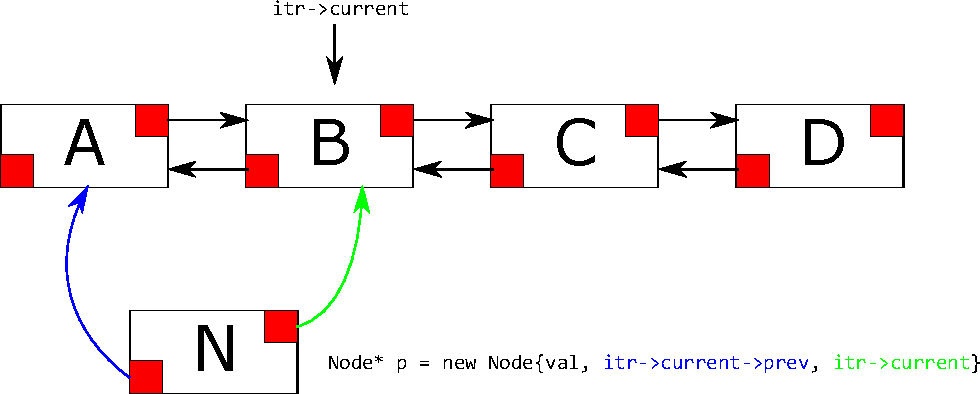
\includegraphics[width=350pt]{./img/List-insert-1.pdf}
\captionof{figure}{\label{fig:org825e867}
Insert a node in a list. Step 1: construct a node}
\end{center}

\begin{center}
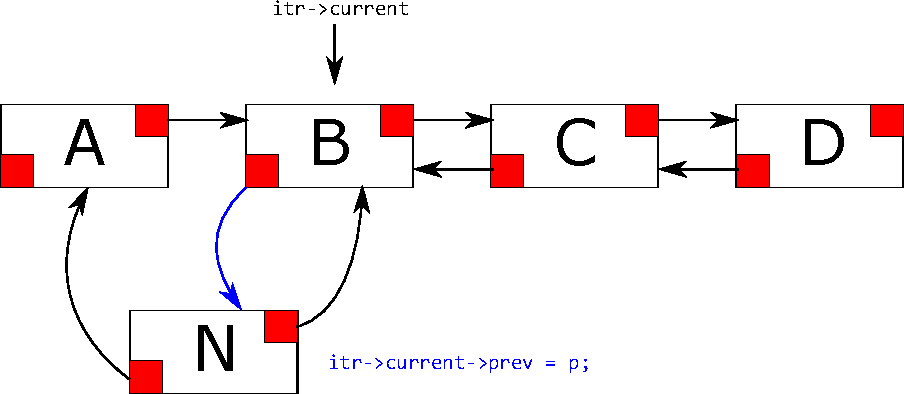
\includegraphics[width=350pt]{./img/List-insert-2.pdf}
\captionof{figure}{\label{fig:orgd400d86}
Insert a node in a list. Step 2: link node}
\end{center}

\begin{center}
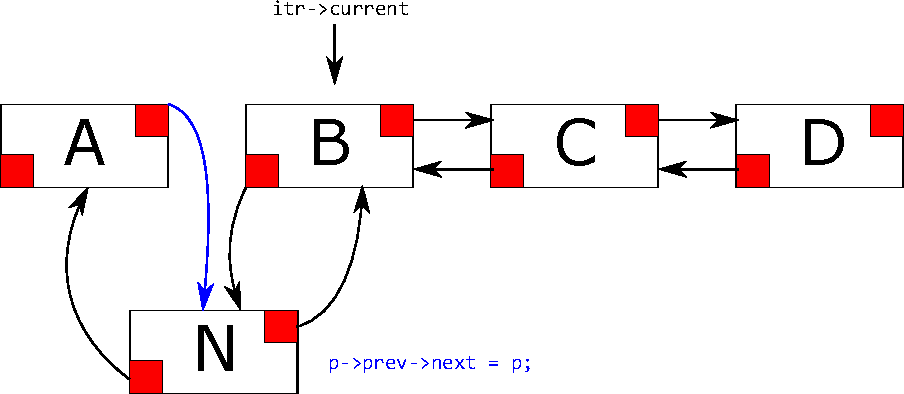
\includegraphics[width=350pt]{./img/List-insert-3.pdf}
\captionof{figure}{\label{fig:orgf2744e2}
Insert a node in a list. Step 3: link node}
\end{center}

The code is as follows:
\begin{minted}[linenos,firstnumber=1,breaklines=true,breakanywhere=true,frame=single,framesep=10pt]{c++}
template <typename T>
typename List<T>::iterator List<T>::insert(iterator itr, const T& val) {
  // update the size of the list
  theSize++; 

  // construct node
  Node* p = new Node{val, itr->current->prev, itr->current};

  // link the node back inti the list
  itr->current->prev = p;
  p->prev->next = p;

  // return an iterator pointing to the inserted element
  // notice that the constructor of iterator which accepts a pointer to a Node has been called implicitly to construct an iterator and return.
  return p;
}
\end{minted}

Notice that we are calling the following constructor of \texttt{iterator}:
\begin{minted}[breaklines=true,breakanywhere=true,frame=single,framesep=10pt]{c++}
iterator(Node* p);
\end{minted}

This is why we need to declare \texttt{List<T>} as friend of our iterator class (this constructor is in protected region).

Move version of insert is similar, except for the use of \texttt{std::move()}. We'll simplify the above code in just one line:
\begin{minted}[linenos,firstnumber=1,breaklines=true,breakanywhere=true,frame=single,framesep=10pt]{c++}
// move version of insert()
template <typename T>
typename List<T>::iterator List<T>::insert(iterator itr, T&& val) {
  theSize++;
  return { (*(itr.current)).prev = ((*(itr.current)).prev)->next = new Node{std::move(val), (*(itr.current)).prev, itr.current} };
}
\end{minted}
\subsection{\texttt{erase()}}
\label{sec:org4cddcc5}
This function accepts an iterator. It will delete the node referenced by the iterator and return the iterator to the next node. Content referenced by \texttt{itr} will be reclaimed by \texttt{delete}. The size of the list will also update. The process of deleting a node in list is shown below.

\begin{center}
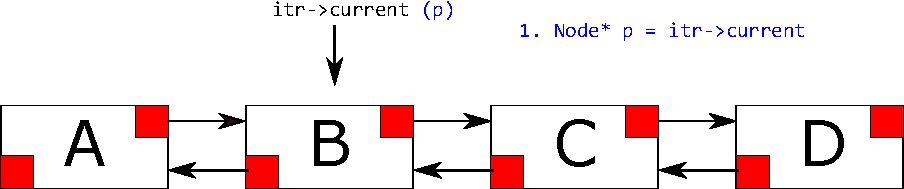
\includegraphics[width=350pt]{./img/List-delete-1.pdf}
\captionof{figure}{\label{fig:orgf35be22}
Delete a node in a list. Step 1: convenient renaming}
\end{center}

\begin{center}
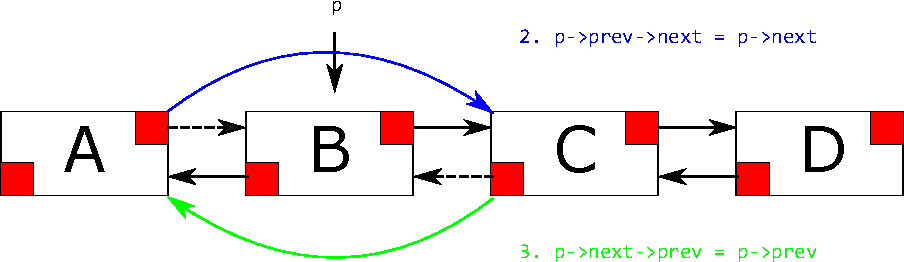
\includegraphics[width=350pt]{./img/List-delete-2.pdf}
\captionof{figure}{\label{fig:orgbe5efee}
Delete a node in a list. Step 2: reconnect node}
\end{center}

\begin{center}
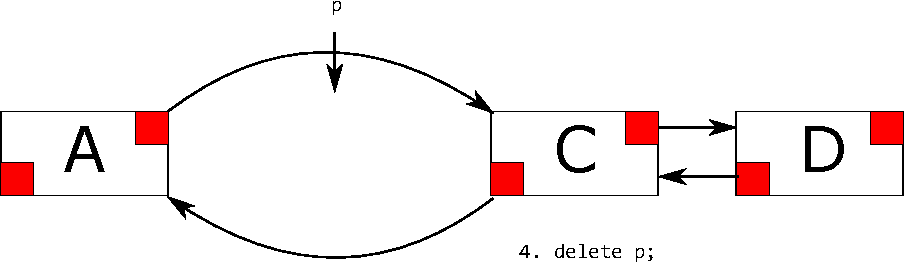
\includegraphics[width=350pt]{./img/List-delete-3.pdf}
\captionof{figure}{\label{fig:orgc50d265}
Delete a node in a list. Step 3: delete node}
\end{center}

Also, pay attention that we want to return an iterator referencing the next node. So we want to keep copy of that first, and return at the end of the function. The code is as follows:
\begin{minted}[linenos,firstnumber=1,breaklines=true,breakanywhere=true,frame=single,framesep=10pt]{c++}
template <typename T>
typename List<T>::iterator List<T>::erase(iterator itr) {
  Node* p = itr.current;
  iterator retVal{ p->next };
  (p->prev)->next = p->next;
  (p->next)->prev = p->prev;
  delete p;
  theSize--;

  return retVal;
}
\end{minted}
\subsection{\texttt{erase()} [range based]}
\label{sec:org19e357a}
We'll call the \texttt{erase()} function we have just defined.
\begin{minted}[linenos,firstnumber=1,breaklines=true,breakanywhere=true,frame=single,framesep=10pt]{c++}
template <typename T>
typename List<T>::iterator List<T>::erase(iterator start, iterator end) {
  for (iterator itr = start; itr != end;)
    itr = erase(itr);

  return end;
}
\end{minted}
\subsection{\texttt{init()}}
\label{sec:org6cd8418}
This function will initialize the data member of an empty \texttt{List} object. It will connect \texttt{head} and \texttt{tail} together.
\begin{minted}[linenos,firstnumber=1,breaklines=true,breakanywhere=true,frame=single,framesep=10pt]{c++}
template <typename T>
void List<T>::init() {
  theSize = 0;
  head = new Node;
  tail = new Node;
  head->next = tail;
  tail->prev = head;
}
\end{minted}
\subsection{Nonclass global functions}
\label{sec:org92533c6}
We also defined some global functions that related to \texttt{List} operations. Pay attention that they are not part of the \texttt{List} class. 
\subsubsection{\texttt{operator==()}}
\label{sec:orge62c4a8}
Two \texttt{List} object is said equal, if they have same number of elements and all the corresponding elements are the same.
\begin{minted}[linenos,firstnumber=1,breaklines=true,breakanywhere=true,frame=single,framesep=10pt]{c++}
template <typename T>
bool cop4530::operator==(const List<T>& lhs, const List<T>& rhs) {
  if (lhs.size() != rhs.size())
    return false;

  for (auto itr_lhs = lhs.begin(), itr_rhs = rhs.begin(); itr_lhs != lhs.end(); ++itr_lhs, ++itr_rhs) {
    if (*itr_lhs != *itr_rhs)
      return false;
  }

  return true;

}
\end{minted}
\subsubsection{\texttt{operator!=()}}
\label{sec:orgc07734d}
Call \texttt{operator==()} to finish the work.
\begin{minted}[linenos,firstnumber=1,breaklines=true,breakanywhere=true,frame=single,framesep=10pt]{c++}
template <typename T>
bool cop4530::operator!=(const List<T>& lhs, const List<T>& rhs) {
  return !(lhs == rhs);
}
\end{minted}
\subsubsection{\texttt{operator<<()}}
\label{sec:org0c08b59}
If implemented globally, \texttt{operator<<()} may not acces the private member of \texttt{List}. I used to declare this function as friend of \texttt{List} inside the header of \texttt{List} class. But actually, you have defined a public interface \texttt{List<T>::print()}, so we can just call that function and pass the \texttt{std::ostream} object. Code:
\begin{minted}[linenos,firstnumber=1,breaklines=true,breakanywhere=true,frame=single,framesep=10pt]{c++}
template <typename T>
std::ostream& cop4530::operator<<(std::ostream& os, const List<T>& l) {
  l.print(os);
  return os;
}
\end{minted}
\chapter{Stack}
\label{sec:orge056c33}
\section{General Idea}
\label{sec:org429ab49}
A stack is a data structure that can manage elements in a \textbf{Last-in-First-out} manner, or \textbf{LIFO}. Stacks are useful data structures for algorithms that work first with the last saved element of a series. For example, you have a program that looks like this:
\begin{minted}[breaklines=true,breakanywhere=true,frame=single,framesep=10pt]{c++}
{
  {
    {
      {
	{
	  // the innermost function is doing something here
	  // local variable created here will be the last in the stack
	  // but will be the first to out the stack
	  // because it will be destroyed when coming out from this block
	}
      }
    }
  }
}
\end{minted}

Stacks can be implemented as an adapter class --- it uses another container as underlying storage container, and we implement routines that support the \textbf{LIFO} behavior.
\section{Simple Implementation}
\label{sec:orgab4c18d}
In this section, I'll implement a stack template. The default underlying container is \texttt{std::deque}, but can be named other. The \texttt{Stack} class will be implemented in namespace cop4530.
\subsection{Outline of \texttt{cop4530::Stack}}
\label{sec:org7efe8e8}
We declare the \texttt{Stack} class as follows:
\begin{minted}[breaklines=true,breakanywhere=true,frame=single,framesep=10pt]{c++}
template <typename T, typename Container = std::deque<T>>
class Stack {

};
\end{minted}

Notice how we declare the default type of container as \texttt{std::deque<T>}. The whole outline of \texttt{cop4530::Stack} is as follows. When we implement the member functions, we can use the corresponding functions of the underlying container. 
\begin{minted}[linenos,firstnumber=1,breaklines=true,breakanywhere=true,frame=single,framesep=10pt]{c++}
#ifndef MY_STACK_H
#define MY_STACK_H
#include <deque>
#include <iostream>


namespace cop4530 {

  /***** class template Stack<T, Container> *****/
  template <typename T, typename Container = std::deque<T>>
  class Stack {
    protected:
      //internal container
      Container c;
      //friend of Stack class
      //https://web.mst.edu/~nmjxv3/articles/templates.html
      template <typename A, typename B>
      friend bool operator==(const Stack<A,B>& lhs, const Stack<A,B>& rhs);      
      template <typename A, typename B>
      friend bool operator<=(const Stack<A,B>& lhs, const Stack<A,B>& rhs);

    public:
      //constructor, destructor, copy constructor, move constructor
      Stack(); //default zero-argument constructor
      ~Stack(); //destructor
      Stack(const Stack<T, Container>& rhs); //copy constructor
      Stack(Stack<T, Container>&& rhs); //move constructor

      // copy and move assignment operator
      Stack<T, Container>& operator=(const Stack<T, Container>& rhs); //copy assignment operator=
      Stack<T, Container>& operator=(Stack<T, Container>&& rhs); //move assignment operator=

      // Member functions
      bool empty() const; //returns true if the Stack contains no elements, and false otherwise
      void clear(); //delete all elements from the stack
      void push(const T& x); //adds x to the Stack, copy version
      void push(T&& x); //adds x to the Stack, move version 
      void pop(); //removes and discards the most recently added element of the Stack 
      T& top(); //returns a reference to the most recently added element of the Stack 
      const T& top() const; //returns a const reference to the most recently added element of the Stack
      int size() const; //returns the number of elements stored in the Stack
      void print(std::ostream& os, char ofc = ' ') const; //print elements of Stack to ostream os; this function prints elements in the opposite order, the oldest element should be printed first (last in last print)            
  };

  /***** Overloading non-member global functions *****/
  template <typename T, typename Container = std::deque<T>>
  std::ostream& operator<<(std::ostream& os, const Stack<T, Container>& a); //invokes the print() method to print the Stack<T, Container> a in the specified ostream    

  template <typename T, typename Container = std::deque<T>>
  bool operator==(const Stack<T, Container>& lhs, const Stack<T, Container>& rhs); // returns true if the two compared Stacks have the same elements, in the same order. 

  template <typename T, typename Container = std::deque<T>>
  bool operator!=(const Stack<T, Container>& lhs, const Stack<T, Container>& rhs); // opposite of operator==()

  template <typename T, typename Container = std::deque<T>>
  bool operator<=(const Stack<T, Container>& lhs, const Stack<T, Container>& rhs); // returns true if every element in Stack lhs is smaller than or equal to the corresponding element of Statck rhs, until the end of lhs is reached

  //include the implementation file 
  #include "stack.hpp"

}// end of namespace cop4530


#endif
\end{minted}
\subsection{\texttt{Stack()} [zero]}
\label{sec:org6e2dcc0}
\begin{minted}[linenos,firstnumber=1,breaklines=true,breakanywhere=true,frame=single,framesep=10pt]{c++}
//use initialization list to call zero-parameter constructor of the internal Container 
template <typename T, typename Container>
Stack<T, Container>::Stack() : c() {}
\end{minted}
\subsection{\texttt{\textasciitilde{}Stack()}}
\label{sec:orga69d901}
\begin{minted}[linenos,firstnumber=1,breaklines=true,breakanywhere=true,frame=single,framesep=10pt]{c++}
//do nothing; destructor of data member (the container c) will be called automatically
template <typename T, typename Container>
Stack<T, Container>::~Stack() {}
\end{minted}
\subsection{\texttt{Stack()} [copy]}
\label{sec:orgf5b10de}
\begin{minted}[linenos,firstnumber=1,breaklines=true,breakanywhere=true,frame=single,framesep=10pt]{c++}
//utilize copy constructor of the internal container
template <typename T, typename Container>
Stack<T, Container>::Stack(const Stack<T, Container>& rhs) : c{rhs.c} {}
\end{minted}
\subsection{\texttt{Stack()} [move]}
\label{sec:org73ad319}
\begin{minted}[linenos,firstnumber=1,breaklines=true,breakanywhere=true,frame=single,framesep=10pt]{c++}
// utilize move constructor of the internal container
template <typename T, typename Container>
Stack<T, Container>::Stack(Stack<T, Container>&& rhs) : c {std::move(rhs).c} {}
\end{minted}
\subsection{\texttt{operator=()} [copy]}
\label{sec:orga7bbfbc}
\begin{minted}[linenos,firstnumber=1,breaklines=true,breakanywhere=true,frame=single,framesep=10pt]{c++}
template <typename T, typename Container>
Stack<T, Container>& Stack<T, Container>::operator=(const Stack<T, Container>& rhs) {
  c = rhs.c; //apply copy assignment operator of the internal container
  return *this;
}
\end{minted}
\subsection{\texttt{operator=()} [move]}
\label{sec:org3d9604e}
template <typename T, typename Container>
Stack<T, Container>\& Stack<T, Container>::operator=(Stack<T, Container>\&\& rhs) \{
  c = std::move(rhs).c;
  return *this;
\}
\subsection{\texttt{empty()}}
\label{sec:org71e51b7}
\begin{minted}[linenos,firstnumber=1,breaklines=true,breakanywhere=true,frame=single,framesep=10pt]{c++}
template <typename T, typename Container>
bool Stack<T,Container>::empty() const {
  return c.empty();
}
\end{minted}
\subsection{\texttt{clear()}}
\label{sec:org91209b2}
template <typename T, typename Container>
void Stack<T,Container>::clear() \{
  c.clear();
\}
\subsection{\texttt{push()}}
\label{sec:org4f1222c}
Copy version:
\begin{minted}[linenos,firstnumber=1,breaklines=true,breakanywhere=true,frame=single,framesep=10pt]{c++}
template <typename T, typename Container>
void Stack<T,Container>::push(const T& x) {
  c.push_back(x);
}
\end{minted}
\subsection{\texttt{pop()}}
\label{sec:org22a1eb2}
\begin{minted}[linenos,firstnumber=1,breaklines=true,breakanywhere=true,frame=single,framesep=10pt]{c++}
template <typename T, typename Container>
void Stack<T,Container>::pop() {
  c.pop_back();
}
\end{minted}
\subsection{\texttt{top()}}
\label{sec:orgb9d0a13}
\begin{minted}[linenos,firstnumber=1,breaklines=true,breakanywhere=true,frame=single,framesep=10pt]{c++}
//const version 
template <typename T, typename Container>
const T& Stack<T,Container>::top() const {
  return c.back();
}
\end{minted}
\subsection{\texttt{top()} reference version}
\label{sec:org0854c21}
\begin{minted}[linenos,firstnumber=1,breaklines=true,breakanywhere=true,frame=single,framesep=10pt]{c++}
template <typename T, typename Container>
T& Stack<T,Container>::top() {
  return c.back();
}
\end{minted}
\subsection{\texttt{size()}}
\label{sec:orga08ad61}
\begin{minted}[linenos,firstnumber=1,breaklines=true,breakanywhere=true,frame=single,framesep=10pt]{c++}
template <typename T, typename Container>
int Stack<T,Container>::size() const {
  return c.size();
}
\end{minted}
\subsection{\texttt{print()}}
\label{sec:org9386590}
\begin{minted}[linenos,firstnumber=1,breaklines=true,breakanywhere=true,frame=single,framesep=10pt]{c++}
template <typename T, typename Container>
void Stack<T,Container>::print(std::ostream& os, char ofc) const {
  //check if the container is empty
  if (empty())
    return;
  //print first element (the oldest element)
  os << c.front();

  //print the rest of elements, if there is any
  for (auto itr = c.begin() + 1; itr != c.end(); ++itr) {
    os << ofc << *itr;
  } 
}
\end{minted}
\subsection{Non-member Global functions}
\label{sec:org860d94f}
For the following functions, we'll implement in different ways. \texttt{operator<<()} will not require access to \texttt{Stack}'s private/protected member, it only calls the \texttt{print()} routine from the \texttt{Stack} class. For other three operators (\texttt{==}, \texttt{!=} and \texttt{<=}), we declare them as friend of \texttt{Stack} class, so they can access private/protected members of \texttt{Stack} class. (it is also possible to define a public function in \texttt{Stack}, and call by these operators).
\subsubsection{\texttt{operator<<()}}
\label{sec:org3ab7f89}
\begin{minted}[linenos,firstnumber=1,breaklines=true,breakanywhere=true,frame=single,framesep=10pt]{c++}
template <typename T, typename Container>
std::ostream& operator<<(std::ostream& os, const Stack<T,Container>& a) {
  a.print(os);
  return os;
}
\end{minted}
\subsubsection{\texttt{operator==()}}
\label{sec:org075481e}
In header of \texttt{Stack}, we declare this function as the friend of \texttt{Stack}:
\begin{minted}[breaklines=true,breakanywhere=true,frame=single,framesep=10pt]{c++}
template <typename A, typename B>
friend bool operator==(const Stack<A, B>& lhs, const Stack<A, B>& rhs);
\end{minted}

Pay attention that, you are declaring a function template as the friend of \texttt{Stack}, so you must provide full description of the header of the function template.

After this, we can implement the function template outside of \texttt{Stack} class:
\begin{minted}[linenos,firstnumber=1,breaklines=true,breakanywhere=true,frame=single,framesep=10pt]{c++}
template <typename T, typename Container>
bool operator==(const Stack<T,Container>& lhs, const Stack<T,Container>& rhs) {
  //check size first
  if (lhs.size() != rhs.size())
    return false;

  for(auto itr_l = lhs.c.begin(), itr_r = rhs.c.begin(); itr_l != lhs.c.end(); ++itr_l, ++itr_r) {
    if (*itr_l != *itr_r)
      return false;
  }

  return true;
}
\end{minted}
\subsubsection{\texttt{operator!=()}}
\label{sec:orgb289c37}
We will call \texttt{operator==()} to finish the work.
\begin{minted}[linenos,firstnumber=1,breaklines=true,breakanywhere=true,frame=single,framesep=10pt]{c++}
template <typename T, typename Container>
bool operator!=(const Stack<T,Container>& lhs, const Stack<T,Container>& rhs) {
  return !(lhs == rhs);
}
\end{minted}
\subsubsection{\texttt{operator<=()}}
\label{sec:orgc934748}
Similarly, we declare this function template as friend of \texttt{Stack}:
\begin{minted}[breaklines=true,breakanywhere=true,frame=single,framesep=10pt]{c++}
template <typename A, typename B>
friend bool operator<=(const Stack<A, B>& lhs, const Stack<A, B>& rhs);
\end{minted}

Then, we implement it outside of \texttt{Stack}:
\begin{minted}[linenos,firstnumber=1,breaklines=true,breakanywhere=true,frame=single,framesep=10pt]{c++}
template <typename T, typename Container>
bool operator<=(const Stack<T,Container>& lhs, const Stack<T,Container>& rhs) {
  //test if the size of lhs is larger than rhs, if so, return false
  if(lhs.size() > rhs.size())
    return false;

  for(auto itr_l = lhs.c.begin(), itr_r = rhs.c.begin(); itr_l != lhs.c.end(); ++itr_l, ++itr_r) {
    //check if the current entry in lhs satisfies the condition
    if (*itr_l > *itr_r)
      return false;
  }

  return true;

}
\end{minted}

\chapter{Queue}
\label{sec:org9e9b9da}
\chapter{Tree}
\label{sec:org37102a5}
\section{Binary Search Tree}
\label{sec:orgd6c81b1}
\subsection{General Idea}
\label{sec:orga4e00f1}
A binary search tree is a binary tree implemented with the following rule: a node's left child is no larger than the node; a node's right child is no smaller than the node; Under this rule, it is clear that the smallest node in binary search tree is the leftmost node, while the largest node is the rightmost node.
\subsection{Simple Implementation}
\label{sec:org6cde362}
In this section, a simple binary search tree template will be implemented. The header of the class would be:
\begin{minted}[breaklines=true,breakanywhere=true,frame=single,framesep=10pt]{c++}
template <typename comparable>
class BinarySearchTree {

};
\end{minted}
\texttt{comparable} is the name of a class that supports comparison by \texttt{operator<()}. Since the building of binary search tree requires ordering of nodes.

The header file of binary search tree class template is as follows:
\begin{minted}[linenos,firstnumber=1,breaklines=true,breakanywhere=true,frame=single,framesep=10pt]{c++}
#pragma once
#include <iostream>

template <typename comparable>
class BinarySearchTree {
private:
  //nested tree node structure
  struct BinaryNode {};

private:
  BinaryNode* root;

private:
  /** private operating functions **/
  ///insert 
  void insert(const comparable& val, BinaryNode* & t); //copy
  void insert(comparable&& val, BinaryNode* & t); //move

  ///remove
  void remove(const comparable& val, BinaryNode* & t);

  ///search 
  BinaryNode* findMin(BinaryNode* t) const;
  BinaryNode* findMax(BinaryNode* t) const;
  bool contains(const comparable& val, BinaryNode* t) const;

  ///utility
  void makeEmpty(BinaryNode* & t);
  void printTree(BinaryNode* t, std::ostream& out) const;
  BinaryNode* clone(BinaryNode* t) const;

public:
  /** Constructor and destructor **/
  BinarySearchTree(); //zero-parameter default constructor
  BinarySearchTree(const BinarySearchTree& rhs); //copy constructor
  BinarySearchTree(BinarySearchTree&& rhs); //move constructor
  ~BinarySearchTree(); //destructor

  /** Assignment operator **/
  BinarySearchTree& operator=(const BinarySearchTree& rhs); //copy
  BinarySearchTree& operator=(BinarySearchTree&& rhs); //move

  /** Public Search Interface **/
  const comparable& findMin() const;
  const comparable& findMax() const;
  bool contains(const comparable& val) const;

  /** Modification of tree **/
  void makeEmpty();
  void insert(const comparable& val);//copy version
  void insert(comparable&& val);//move version
  void remove(const comparable& val);

  /** Utility **/
  bool isEmpty() const;
  void printTree(std::ostream& out = std::cout) const;  

};

//include implementation here 
#include "bst.hpp"
\end{minted}

An object of \texttt{BinarySearchTree} class holds a private data member \texttt{root}, which is a pointer to \texttt{TreeNode} type, holds the address of the root of a binary tree. The implementation of \texttt{TreeNode} structure and other member functions are detailed below.

\subsubsection{Tree node structure}
\label{sec:org808d683}
A tree node contains three data members, one is \texttt{comparable} type and is used to hold the data of that node. The other two are pointer to tree node, which will be used to hold the address of the node's left and right child. Code:
\begin{minted}[linenos,firstnumber=1,breaklines=true,breakanywhere=true,frame=single,framesep=10pt]{c++}
struct BinaryNode {
  comparable element;//data stored in the node, and it is comparable (at least one comparable routine is defined for this type)
  BinaryNode* left;
  BinaryNode* right;

  ///constructor
  //copy
  BinaryNode(const comparable& val = val{}, BinaryNode* lt = nullptr, BinaryNode* rt = nullptr) : element {val}, left {lt}, right {rt} {}
  //move
  BinaryNode(comparable&& val = val{}, BinaryNode* lt = nullptr, BinaryNode* rt = nullptr) : element {std::move(val)}, left {lt}, right {rt} {}
};
\end{minted}

\subsubsection{\texttt{zero parameter constructor}}
\label{sec:org6b8b31e}
Just initialize \texttt{root} pointer as \texttt{nullptr}. Code:
\begin{minted}[linenos,firstnumber=1,breaklines=true,breakanywhere=true,frame=single,framesep=10pt]{c++}
template <typename comparable>
BinarySearchTree<comparable>::BinarySearchTree() : root {nullptr} {}
\end{minted}

\subsubsection{\texttt{copy constructor}}
\label{sec:org80fc9bc}
This constructor accepts another object of \texttt{BinarySearchTree} class. It will call an internal recursive routine \texttt{clone()} to finish copying and building. The details of the process is in \texttt{clone()} function. Code:
\begin{minted}[linenos,firstnumber=1,breaklines=true,breakanywhere=true,frame=single,framesep=10pt]{c++}
template <typename comparable>
BinarySearchTree<comparable>::BinarySearchTree(const BinarySearchTree& rhs) {
  root = clone(rhs.root);
}
\end{minted}

\subsubsection{\texttt{move constructor}}
\label{sec:org0f52297}
It is very simple to move, we just need to ``bring'' rhs's root to our root, and redirect \texttt{rhs.root} to \texttt{nullptr}. Code:
\begin{minted}[linenos,firstnumber=1,breaklines=true,breakanywhere=true,frame=single,framesep=10pt]{c++}
template <typename comparable>
BinarySearchTree<comparable>::BinarySearchTree(BinarySearchTree&& rhs) {
  root = rhs.root;
  rhs.root = nullptr;
}
\end{minted}

\subsubsection{\texttt{destructor}}
\label{sec:org157d77b}
Just call \texttt{makeEmpty()} routine, all memories will be recycled. Code:
\begin{minted}[linenos,firstnumber=1,breaklines=true,breakanywhere=true,frame=single,framesep=10pt]{c++}
template <typename comparable>
BinarySearchTree<comparable>::~BinarySearchTree() {
  makeEmpty();
}
\end{minted}

\subsubsection{\texttt{copy assignment operator}}
\label{sec:orgd155ea9}
We call \texttt{clone()} to do the copy and building work. Since this is assignment operator, don't forget return value. Code:
\begin{minted}[linenos,firstnumber=1,breaklines=true,breakanywhere=true,frame=single,framesep=10pt]{c++}
template <typename comparable>
BinarySearchTree<comparable>& BinarySearchTree<comparable>::operator=(const BinarySearchTree& rhs) {
  root = clone(rhs.root);
  return *this;
}
\end{minted}

\subsubsection{\texttt{move assignment operator}}
\label{sec:org65c71d2}
Take \texttt{rhs}'s root directly. Remember the return. Code:
\begin{minted}[linenos,firstnumber=1,breaklines=true,breakanywhere=true,frame=single,framesep=10pt]{c++}
template <typename comparable>
BinarySearchTree<comparable>& BinarySearchTree<comparable>::operator=(BinarySearchTree&& rhs) {
  root = rhs.root;
  rhs.root = nullptr;
  return *this;
}
\end{minted}

\subsubsection{public \texttt{findMin()}}
\label{sec:org6ddf514}
This function is in \texttt{public} domain. It will return the constant reference of the minimum node in the tree. Like many other public member functions, this function will call a private version of \texttt{findMin()} to actually finish the job. This is because of the recursive nature of the tree data structure, many functions will work recursively. Code:
\begin{minted}[linenos,firstnumber=1,breaklines=true,breakanywhere=true,frame=single,framesep=10pt]{c++}
template <typename comparable>
const comparable& BinarySearchTree<comparable>findMin() const {
  return (findMin(root))->element;
}
\end{minted}

\subsubsection{public \texttt{findMax()}}
\label{sec:orga158aa8}
Similar with \texttt{findMin()}. Code:
\begin{minted}[linenos,firstnumber=1,breaklines=true,breakanywhere=true,frame=single,framesep=10pt]{c++}
template <typename comparable>
const comparable& BinarySearchTree<comparable>::findMax() const {
  return (findMax(root))->element;
}
\end{minted}

\subsubsection{public \texttt{contains()}}
\label{sec:orgc24b1c7}
This function accepts a parameter \texttt{val} of type \texttt{comparable}. It will search the tree for the existence of \texttt{val}. It will call a private recursive version of \texttt{contains()}. Code:
\begin{minted}[linenos,firstnumber=1,breaklines=true,breakanywhere=true,frame=single,framesep=10pt]{c++}
template <typename comparable>
bool BinarySearchTree<comparable>::contains(const comparable& val) const {
  return contains(val, root);
}
\end{minted}

\subsubsection{public \texttt{makeEmpty()}}
\label{sec:org850faee}
This function will clear all nodes (reclaim their memory) in the tree. It will call a private recursive version of \texttt{makeEmpty()}. Code:
\begin{minted}[linenos,firstnumber=1,breaklines=true,breakanywhere=true,frame=single,framesep=10pt]{c++}
template <typename comparable>
void BinarySearchTree<comparable>::makeEmpty() {
  makeEmpty(root);
}
\end{minted}

\subsubsection{public \texttt{insert()}}
\label{sec:orgdb79281}
This function accepts a parameter \texttt{val} of type \texttt{comparable}. It will call a private recursive version of \texttt{insert()} to insert \texttt{val} into the tree (to the proper position where \texttt{val} should go). Code (copy version):
\begin{minted}[linenos,firstnumber=1,breaklines=true,breakanywhere=true,frame=single,framesep=10pt]{c++}
template <typename comparable>
void BinarySearchTree<comparable>::insert(const comparable& val) {
  insert(val, root);
}
\end{minted}

\subsubsection{public \texttt{remove()}}
\label{sec:org68e4978}
This function accepts a parameter \texttt{val} of type \texttt{comparable}. It will call a private recursive version of \texttt{remove()} to remove \texttt{val} from the tree. Code:
\begin{minted}[linenos,firstnumber=1,breaklines=true,breakanywhere=true,frame=single,framesep=10pt]{c++}
template <typename comparable>
void BinarySearchTree<comparable>::remove(const comparable& val) {
  remove(val, root);
}
\end{minted}

\subsubsection{public \texttt{isEmpty()}}
\label{sec:org0c77c8c}
This function will check if the tree is empty. The criteria is simple: if the root is \texttt{nullptr}, then the tree is empty. Code:
\begin{minted}[linenos,firstnumber=1,breaklines=true,breakanywhere=true,frame=single,framesep=10pt]{c++}
template <typename comparable>
bool BinarySearchTree<comparable>::isEmpty() const {
  if (root == nullptr)
    return true;
  else 
    return false;
}
\end{minted}

\subsubsection{public \texttt{printTree()}}
\label{sec:org84fc3d4}
This function accepts a \texttt{std::ostream} object \texttt{out}. It will call a private version of \texttt{printTree()} and pass this object into it, to print the tree in in-order (in ascending order). Code:
\begin{minted}[linenos,firstnumber=1,breaklines=true,breakanywhere=true,frame=single,framesep=10pt]{c++}
template <typename comparable>
void BinarySearchTree<comparable>::printTree(std::ostream& out) const {
  printTree(root, out);
} 
\end{minted}

\subsubsection{\texttt{insert()}}
\label{sec:orge7221e2}
The private recursive version of \texttt{insert()}. Implemented recursively. It accepts two parameters: a \texttt{comparable} type \texttt{val}, and a pointer to \texttt{TreeNode} type \texttt{t}. The function can insert the value into the subtree whose root is indicated by \texttt{t}. Its working steps are:
\begin{itemize}
\item check if \texttt{t} is pointing to \texttt{nullptr}, if so, this is the base case: an empty branch is found, and \texttt{val} should be inserted there;
\item if it is not the base case, we will insert it into \texttt{t}'s children:
\begin{itemize}
\item \texttt{val > t->element}: insert to right subtree by calling itself and pass \texttt{val} and \texttt{t->right}
\item \texttt{val < t->element}: insert to left subtree by calling itself and pass \texttt{val} and \texttt{t->right}
\end{itemize}
\item if \texttt{val == t->element}, we do nothing, since its already in the tree (no duplicate)
\end{itemize}

Code (copy version):
\begin{minted}[linenos,firstnumber=1,breaklines=true,breakanywhere=true,frame=single,framesep=10pt]{c++}
template <typename comparable>
void BinarySearchTree<comparable>::insert(const comparable& val, BinaryNode* & t) {  
  //base case1: t is pointing to nullptr
  if (t == nullptr) {
    t = new BinaryNode{val}; //this step will modify t, so pass the pointer by reference is necessary
    return;
  }

  //determine which branch to insert 
  //not considering the equal case 
  if (val < t->element)
    insert(val, t->left);
  else if (val > t->element)
    insert(val, t->right);
  else
    return;//val == t->element, do nothing
}
\end{minted}

Notice that the passed in \texttt{TreeNode} pointer type is referenced type, this is because we will change the memory address stored in pointer itself when we allocate new chunk of memory and store the new tree node.

\subsubsection{\texttt{remove()}}
\label{sec:orga79c5d3}
This is internal private version of \texttt{remove()}. It accepts two parameters: a \texttt{comparable} type \texttt{val}, a reference to pointer of \texttt{TreeNode} type (we need to change the address stored in pointer, so we need reference type pointer). This function works recursively. It will remove the node containing \texttt{val} in subtree whose root is pointed by \texttt{t}. When we remove a node from the tree, its children are disconnected from the tree (because this node connects them to the tree). We need to reconnect them to the tree. The details of reconnecting protocol is up to programmer's choice, here we'll introduce a simple way.
\begin{itemize}
\item there are four base cases
\begin{enumerate}
\item \texttt{t == nullptr}: no match found, return
\item \texttt{t->element > val}: call \texttt{remove(val, t->left)}
\item \texttt{t->element < val}: call \texttt{remove(val, t->right)}
\item \texttt{t->element == val}: this is the node we want to remove, proceed to next step
\end{enumerate}
\item find the left most leaf of \texttt{t->right}: \texttt{left\_leaf\_ptr}
\item attach \texttt{t->left} to the left child of \texttt{left\_leaf\_ptr}
\item use a temporary \texttt{TreeNode} pointer \texttt{temp}  to store address of \texttt{t->right}
\item reclaim \texttt{t}'s memory
\item reconnect previous \texttt{t}'s children by: \texttt{t = temp}. Notice that \texttt{t} should point to its parent's children. Before deletion, \texttt{t}'s parent's child is \texttt{t}, now, \texttt{t}'s parent's child is \texttt{t->right}, \texttt{t->left} is also connected to \texttt{t->right}.
\end{itemize}

Code:
\begin{minted}[linenos,firstnumber=1,breaklines=true,breakanywhere=true,frame=single,framesep=10pt]{c++}
template <typename comparable>
void BinarySearchTree<comparable>::remove(const comparable& val, BinaryNode* & t) {
  //base case 1: t is pointing to nullptr, no match
  if (t == nullptr)
    return;

  //base case 2: t is pointing to the target node
  if (t->element == val) {
    //find the left most spot of t->right, and attach t->left to it
    if (t->right == nullptr) {
      t->right = t->left;
    }

    else {
      BinaryNode* left_leaf_ptr = t->right;
      while (left_leaf_ptr -> left != nullptr)
	left_leaf_ptr = left_leaf_ptr -> left;
      //after the above loop, left_leaf_ptr is pointing to the left most leaf of t->right, attach t->left to the left subtree of this leaf
      left_leaf_ptr -> left = t->left;
    }

    //keep record of the address of current t->right
    BinaryNode* temp = t->right;
    //reclaim memory 
    delete t;
    //re-connect tree node 
    t = temp; // here requires modifying t, thus reference is required

    return;
  }

  //t is not pointing to the target node
  if (t->element > val) 
    remove(val, t->left);
  else
    remove(val, t->right);
}
\end{minted}

\subsubsection{\texttt{findMin()}}
\label{sec:orgf21fea3}
This function will return a pointer of \texttt{TreeNode} type which points to the left most leaf of the tree whose root is pointed by the passed in \texttt{TreeNode} pointer \texttt{t}. If \texttt{t == nullptr}, \texttt{nullptr} will be returned. Code:
\begin{minted}[linenos,firstnumber=1,breaklines=true,breakanywhere=true,frame=single,framesep=10pt]{c++}
template <typename comparable>
typename BinarySearchTree<comparable>::BinaryNode* BinarySearchTree<comparable>::findMin(BinaryNode* t) const {
  if (t == nullptr)
    return t;

  while (t->left != nullptr)
    t = t->left;
  //after the above loop, t is now pointing to left-most leaf
  return t;  
}
\end{minted}

Pay attention to the return type keyword:
\begin{minted}[breaklines=true,breakanywhere=true,frame=single,framesep=10pt]{c++}
typename BinarySearchTree<comparable>::BinaryNode*
\end{minted}
If you are returning a nested class type, for example, in the above code you are returning a pointer to \texttt{BinaryNode}, which itself is a structure defined in \texttt{BinarySearchTree}, you have to add the keyword \texttt{typename} to indicate this is a type to be returned.

\subsubsection{\texttt{findMax()}}
\label{sec:org6c33701}
Similar with \texttt{findMin()}, this function will return a pointer to the right most node. Code:
\begin{minted}[linenos,firstnumber=1,breaklines=true,breakanywhere=true,frame=single,framesep=10pt]{c++}
template <typename comparable>
typename BinarySearchTree<comparable>::BinaryNode* BinarySearchTree<comparable>::findMax(BinaryNode* t) const {
  if (t == nullptr)
    return t;

  while (t->right != nullptr)
    t = t->right;
  //after the above loop, t is not pointing to right-most leaf
  return t;   
}
\end{minted}

\subsubsection{\texttt{contains()}}
\label{sec:orga9f6b6f}
Steps to find a specific node is similar with \texttt{remove()}. Code:
\begin{minted}[breaklines=true,breakanywhere=true,frame=single,framesep=10pt]{c++}
template <typename comparable>
bool BinarySearchTree<comparable>::contains(const comparable& val, BinaryNode* t) const {
  //base case: t == nullptr, no match found
  if (t == nullptr)
    return false;

  //base case2: t->element == val
  if (t->element == val)
    return true;

  //try to find val in t's children
  if (t->element > val)
    return contains(val, t->left);
  else 
    return contains(val, t->right);
}
\end{minted}

\subsubsection{\texttt{makeEmpty()}}
\label{sec:org0236142}
This function accepts a pointer of \texttt{TreeNode} type \texttt{t}. It will reclaim all memory used by this node and all its children. Working steps:
\begin{itemize}
\item check if base case reached (\texttt{t == nullptr}), if so, do nothing, return
\item call itself and pass \texttt{t->left} to reclaim memory of its left child
\item call itself and pass \texttt{t->right} to reclaim memory of its right child
\item reclaim \texttt{t}'s memory, and assign it to \texttt{nullptr}
\end{itemize}

Code:
\begin{minted}[linenos,firstnumber=1,breaklines=true,breakanywhere=true,frame=single,framesep=10pt]{c++}
template <typename comparable>
void BinarySearchTree<comparable>::makeEmpty(BinaryNode* & t) {
  //base case 
  if (t == nullptr)
    return;

  //begin makeEmpty
  makeEmpty(t->left);
  makeEmpty(t->right);
  delete t;
  t = nullptr;
}
\end{minted}

\subsubsection{\texttt{printTree()}}
\label{sec:orga36c71a}
The idea is similar with \texttt{makeEmpty()}, the only difference is in \texttt{printTree}, you are printing rather than deleting. Code:
\begin{minted}[linenos,firstnumber=1,breaklines=true,breakanywhere=true,frame=single,framesep=10pt]{c++}
template <typename comparable>
void BinarySearchTree<comparable>::printTree(BinaryNode* t, std::ostream& out) const {
  //base case 
  if (t == nullptr)
    return;

  //print the tree in inorder traversal
  printTree(t->left, out);
  out << t->element << ' ';
  printTree(t->right, out);
}
\end{minted}

\subsubsection{\texttt{clone()}}
\label{sec:org31862ef}
This function accepts a pointer to \texttt{TreeNode} type \texttt{t}. It will return a pointer to a newly constructed \texttt{TreeNode}, whose element is the same as \texttt{t->element}, left child is the same as \texttt{t->left}, right child is the same as \texttt{t->right}. It works in a recursive way. Code:
\begin{minted}[linenos,firstnumber=1,breaklines=true,breakanywhere=true,frame=single,framesep=10pt]{c++}
typename BinarySearchTree<comparable>::BinaryNode* BinarySearchTree<comparable>::clone(BinaryNode* t) const {
  /** pay attention that what you clone is a BinaryNode! **/
  //base case 
  if (t == nullptr)
    return t;

  //clone 
  return new BinaryNode{t->element, clone(t->left), clone(t->right)};
}
\end{minted}

Pay attention that, the returned pointer is constructed by the address generated by the \texttt{new} operation (allocating new memory spaces).

\subsection{Problem with Simple Binary Search Tree}
\label{sec:org9bde72f}
The binary search tree can only guarantee \(O(\log{N})\) complexity when the tree is nearly \textbf{BALANCED}, which means for any node in the binary search tree, the number of nodes in its left subtree is roughly the same as its right subtree. However, this may not be the case during practical uses of this simple binary search tree. Consider two cases:
\begin{enumerate}
\item We insert an ordered array into the tree by calling \texttt{insert()} repeatedly for all the elements in array in order. We'll create a linked list rather than a binary tree. If its in ascending order, only right subtree will be used; If its in descending order, only left subtree will be used. Many operations will be \(O(N)\) complexity.
\item We have a balanced binary search tree at first. We kept removing nodes in it by calling \texttt{remove()}. In our implementation of \texttt{remove()}, we will attach the target node's left subtree to its right subtree. So this will decrease the number of nodes in left subtrees. The balanced tree will degenerate to un-balanced tree, with one subtree holds significant more amount of nodes than the other subtree.
\end{enumerate}

In both cases, we may face increased time complexity. Thus, we want to come up with ways to build \textbf{balanced} binary search tree.

\section{AVL Tree}
\label{sec:org55f5f7a}
\subsection{General Idea}
\label{sec:org35bc09b}
An AVL tree is identical to a binary search tree, except that for every node in the tree, the height of the left and right subtrees can differ by most 1 (the height of an empty tree is defined to be -1).

Let \(S(h)\) be the minimum number of nodes that an AVL tree of height \(h\) needs. Then we have: \(S(h) = S(h - 1) + S(h - 2) + 1\), where \(S(h - 1)\) is the number of nodes of the higher child of \texttt{root}, \(S(h - 2)\) is the number of nodes of the lower child of \texttt{root}, 1 corresponds to one layer from child to \texttt{root}.
\subsection{AVL-property Loss and Fix}
\label{sec:orge6b7ec6}
In this section, we'll talk about the cause of AVL-property loss and ways to fix it. Both insertion and deletion operation can violate AVL-property, since they can bring height change to the tree. We'll analyze them one by one.
\subsubsection{Insertion caused unbalance and fix}
\label{sec:org70b7661}
In Figure \ref{fig:org96450ae}, before insertion, N's left and right subtree's height was already differred by 1 (dashed line indicates possible insertion site). After a node is inserted into one of its subtree (LL, LR, RL, RR), the height of N's left and right subtree is now differred by two, AVL property lost for node N. There are four possible cases:
\begin{enumerate}
\item Insert into \texttt{N->left->left} (insert into LL)
\item Insert into \texttt{N->left->right} (insert into LR)
\item Insert into \texttt{N->right->left} (insert into RL)
\item Insert into \texttt{N->right->right} (insert into RR)
\end{enumerate}


\begin{center}
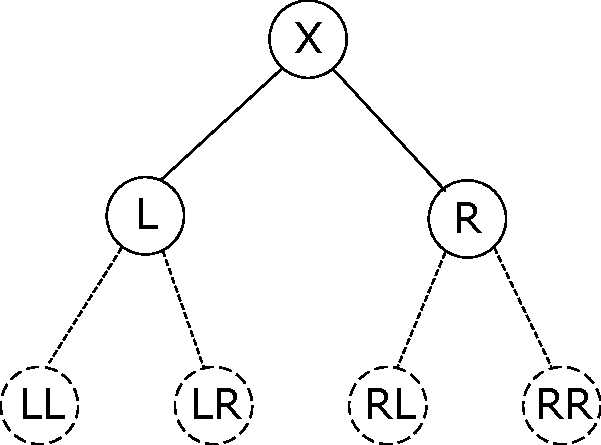
\includegraphics[width=200pt]{./img/AVL-illustration.pdf}
\captionof{figure}[Figure]{\label{fig:org96450ae}
AVL tree illustration}
\end{center}

Case 1 and case 4 are illustrated in a greater detail in Figure \ref{fig:orgc165b0f}. Case 2 and case 3 are illustrated in a greater detail in Figure \ref{fig:orgaed53a5}.

\begin{center}
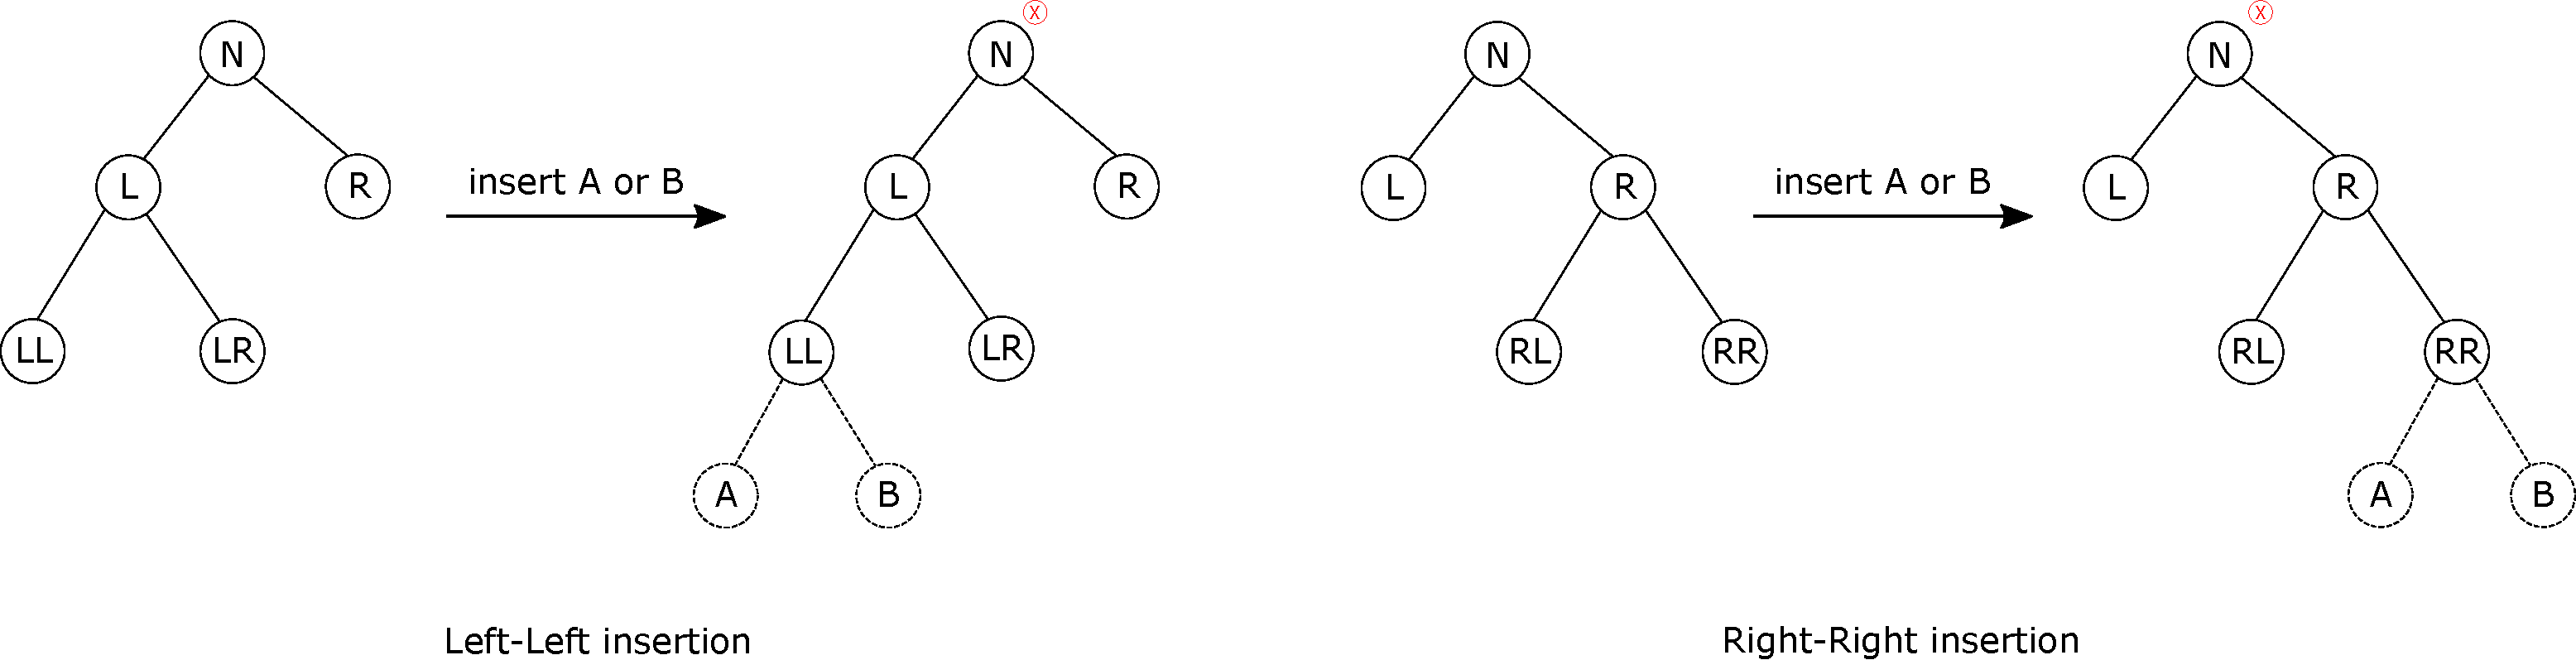
\includegraphics[width=500pt]{./img/AVL-LL-RR-insertion.pdf}
\captionof{figure}[Figure]{\label{fig:orgc165b0f}
Left-left insertion and right-right insertion}
\end{center}

\begin{center}
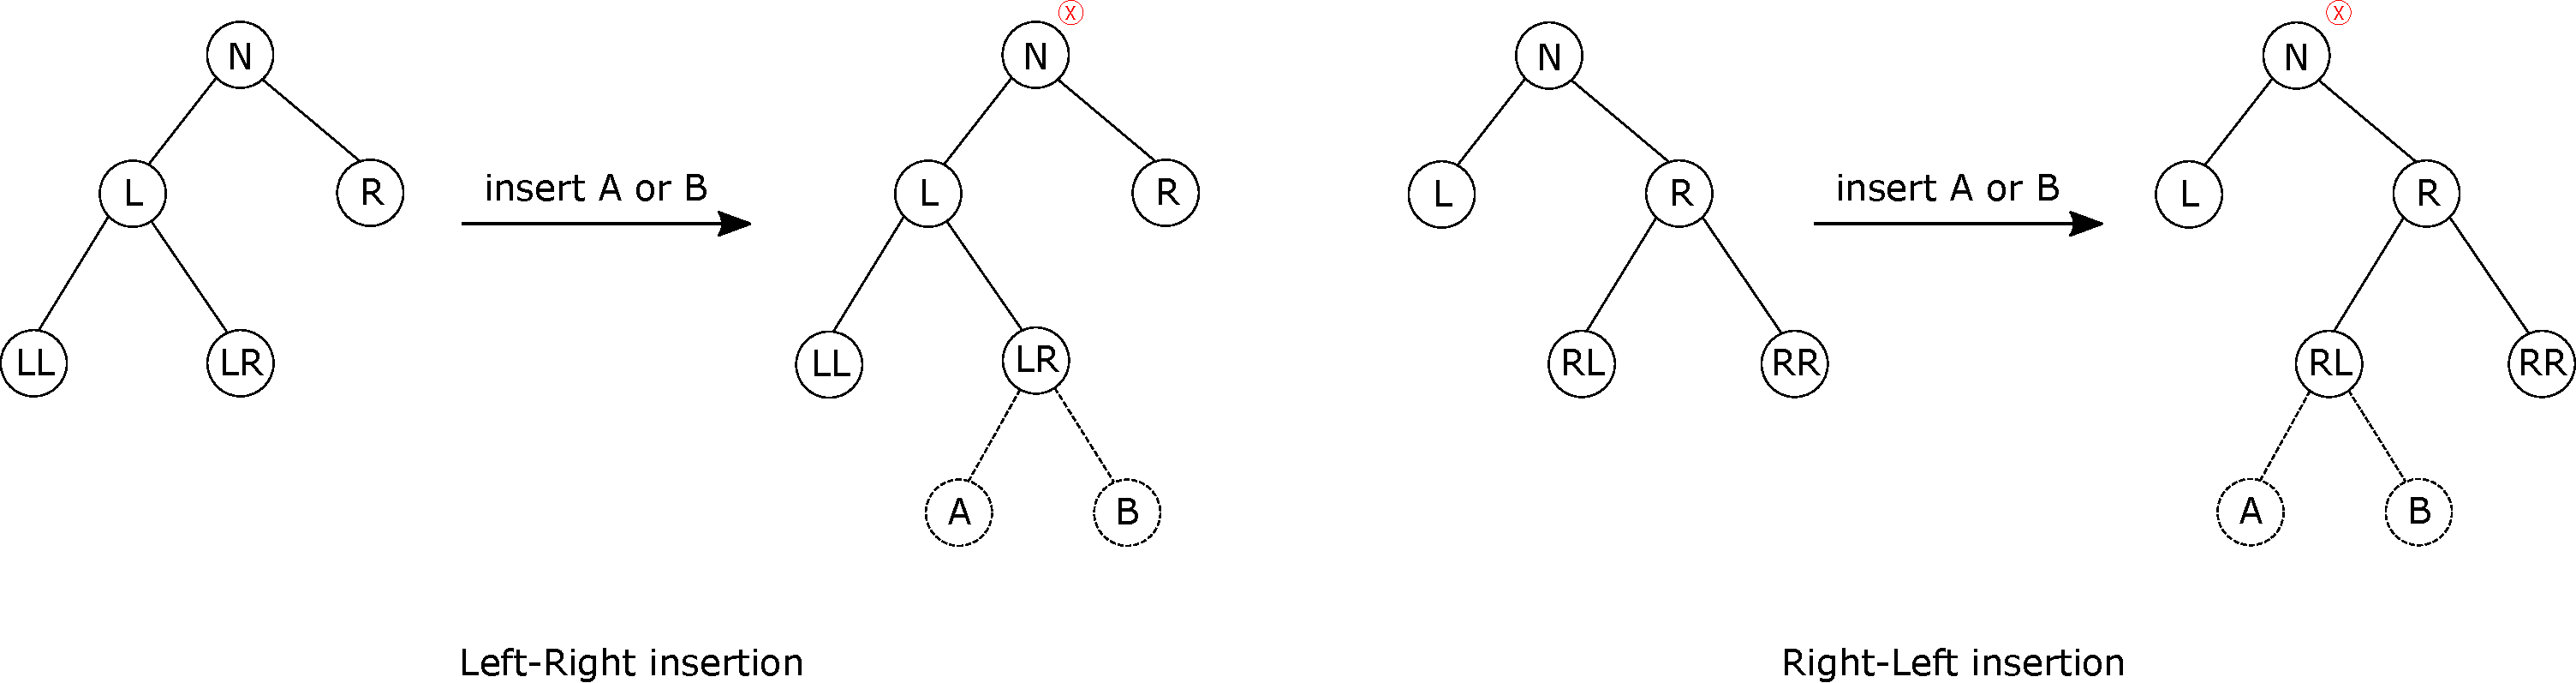
\includegraphics[width=500pt]{./img/AVL-LR-RL-insertion.pdf}
\captionof{figure}[Figure]{\label{fig:orgaed53a5}
Left-right insertion and right-left insertion}
\end{center}

One thing should be pointed out is that, after an insertion, only nodes that are on the path from the insertion point to the root might have their AVL-property lost, because only those nodes have their subtrees altered. And we only need to fix the first node who lost AVL-property, so the rest nodes above it can restore their AVL-property.

To fix AVL-property loss by LL-insertion and RR-insertion, we can perform a single rotation. Specifically:
\begin{itemize}
\item to fix LL-insertion, we rotate node \texttt{N} with its left child. In this process, \texttt{N} will become \texttt{N->left}'s right child, while \texttt{N->left}'s right child will become \texttt{N}'s left child.
\item to fix RR-insertion, we rotate node \texttt{N} with its right child. In this process, \texttt{N} will become \texttt{N->right}'s left child, while \texttt{N->right}'s left child will become \texttt{N}'s right child.
\end{itemize}

The process is illustrated in Figure \ref{fig:org8237354}. The letters in node represents the original position of the node.

\begin{figure}[htbp]
\centering
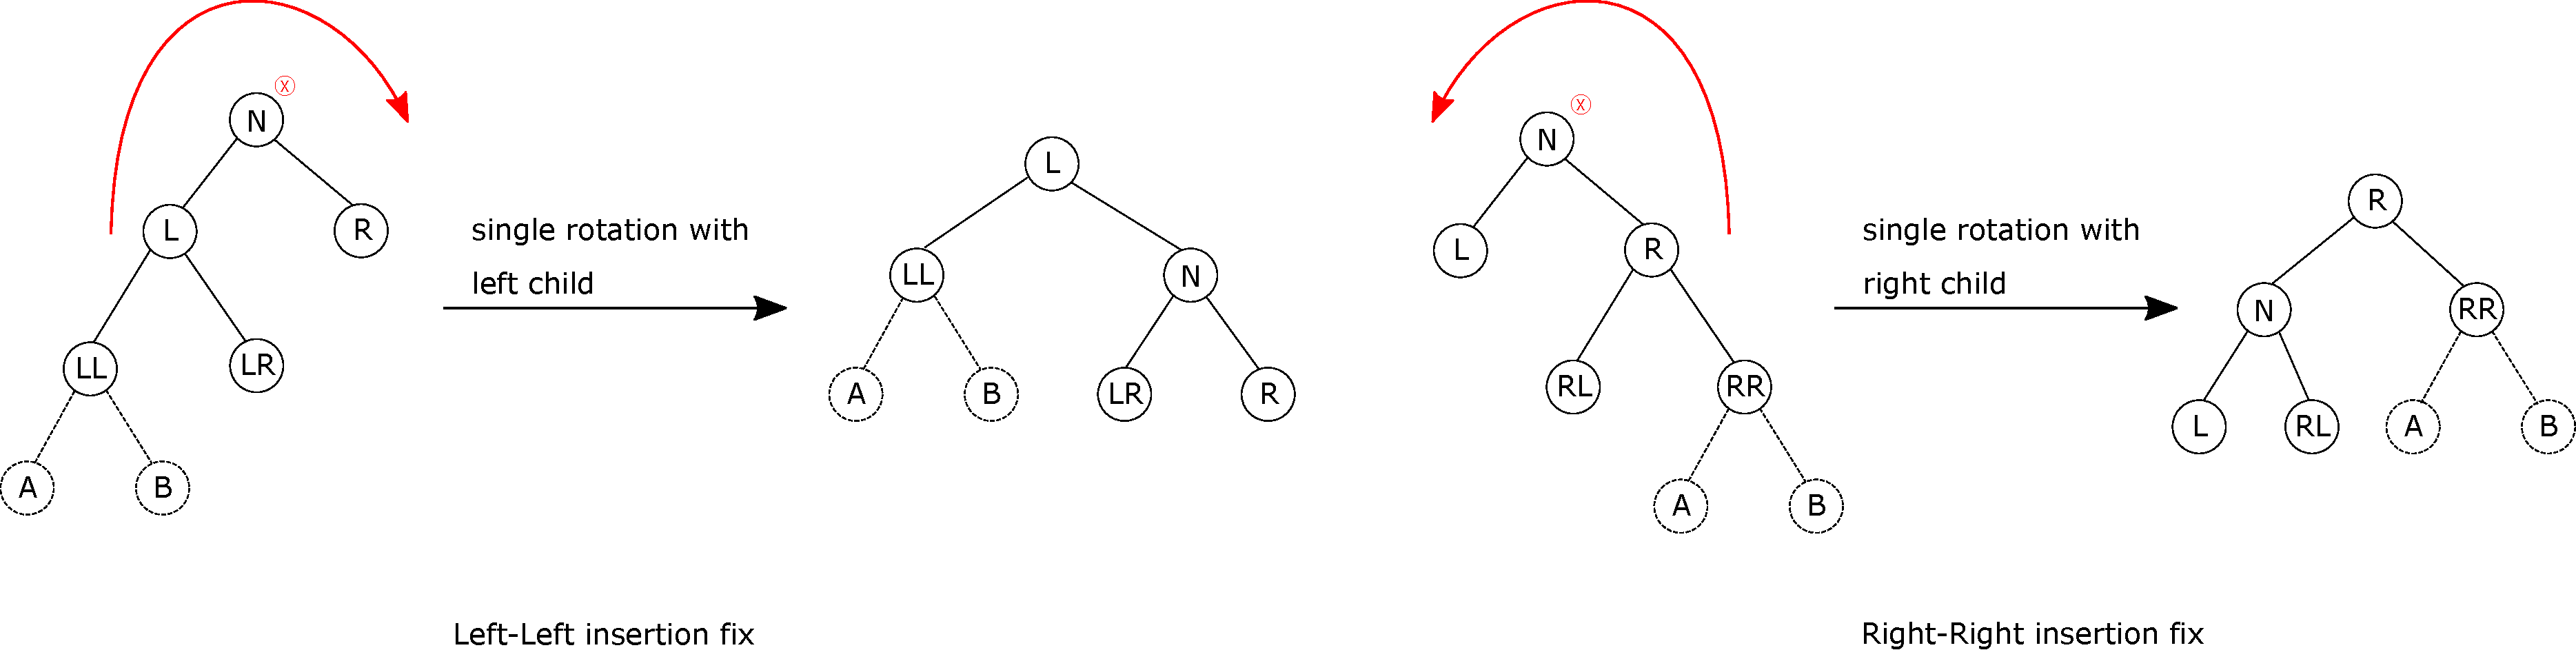
\includegraphics[width=500pt]{./img/AVL-LL-RR-insertion-fix.pdf}
\caption[Figure]{\label{fig:org8237354}
Single rotation to fix AVL-property loss caused by Left-left insertion and right-right insertion}
\end{figure}

From Figure \ref{fig:org8237354}, we can see that single rotation can modify the height of node \texttt{LL} or \texttt{RR}, no matter \texttt{A} or \texttt{B} is inserted.


To fix AVL-property loss by LR-insertion and RL-insertion, we have to perform two rotations. Specifically:
\begin{itemize}
\item to fix LR-insertion
\begin{itemize}
\item rotate \texttt{N->left} with \texttt{N->left}'s right child (single rotation)
\item rotate \texttt{N} with \texttt{N}'s left child (single rotation)
\end{itemize}
\item to fix RL-insertion
\begin{itemize}
\item rotate \texttt{N->right} with \texttt{N->right}'s left child (single rotation)
\item rotate \texttt{N} with \texttt{N}'s right child (single rotation)
\end{itemize}
\end{itemize}

The process to fix LR-insertion is illustrated in Figure \ref{fig:org933a468}. The process to fix RL-insertion is illustrated in Figure \ref{fig:org6fc9e78}.

\begin{figure}[htbp]
\centering
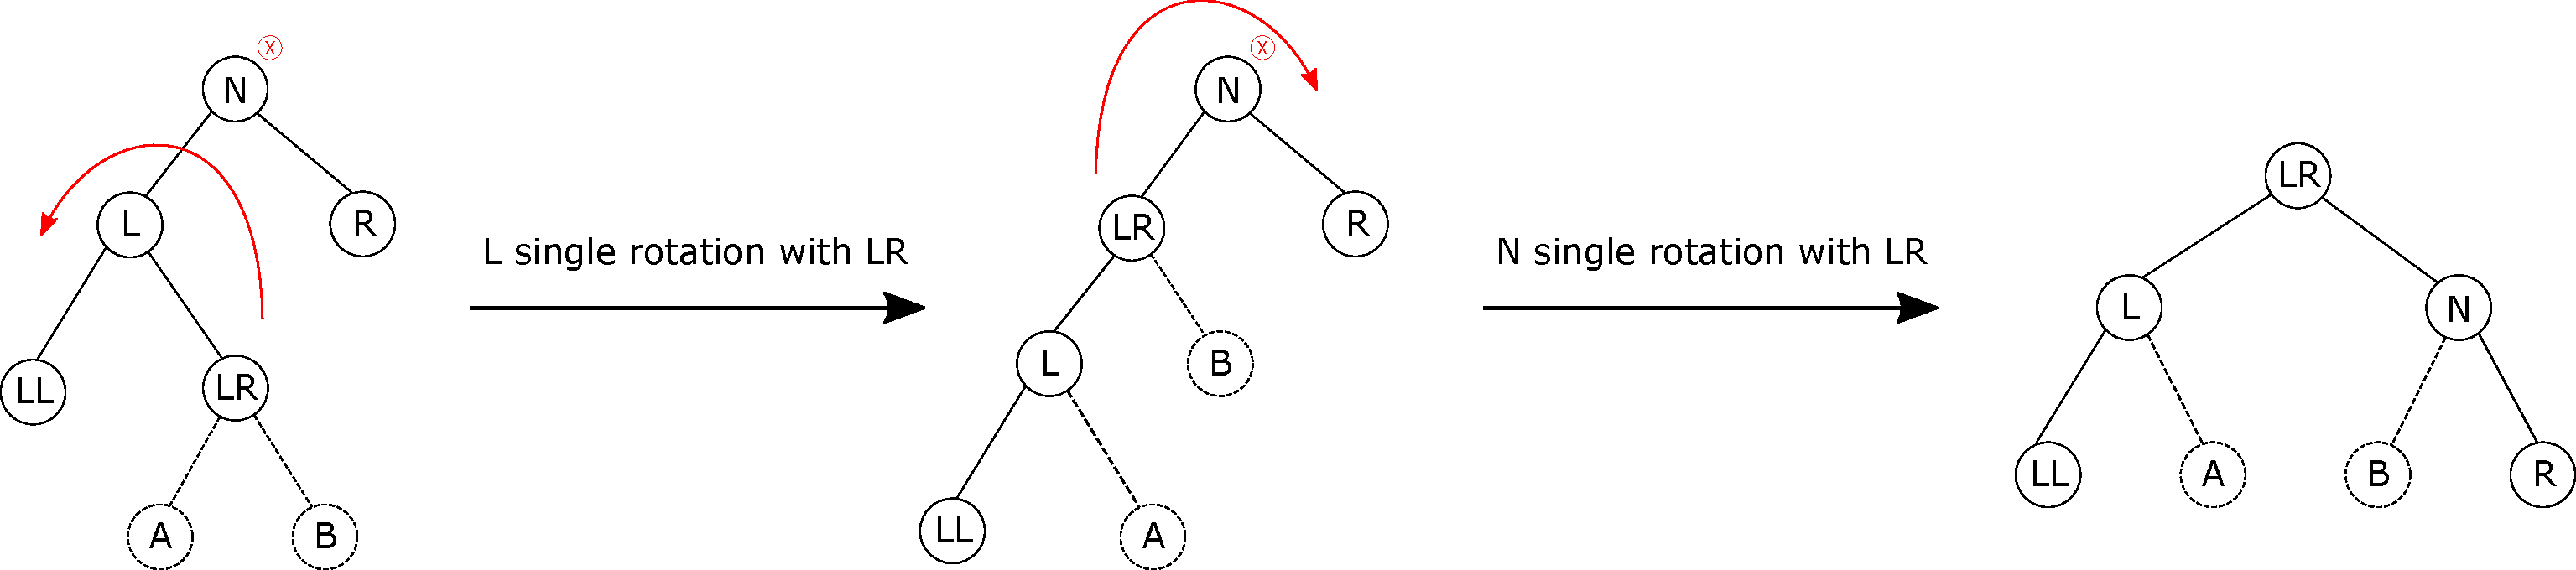
\includegraphics[width=400pt]{./img/AVL-LR-insertion-fix.pdf}
\caption[Figure]{\label{fig:org933a468}
Double rotation to fix AVL-property loss caused by Left-right insertion}
\end{figure}

\begin{figure}[htbp]
\centering
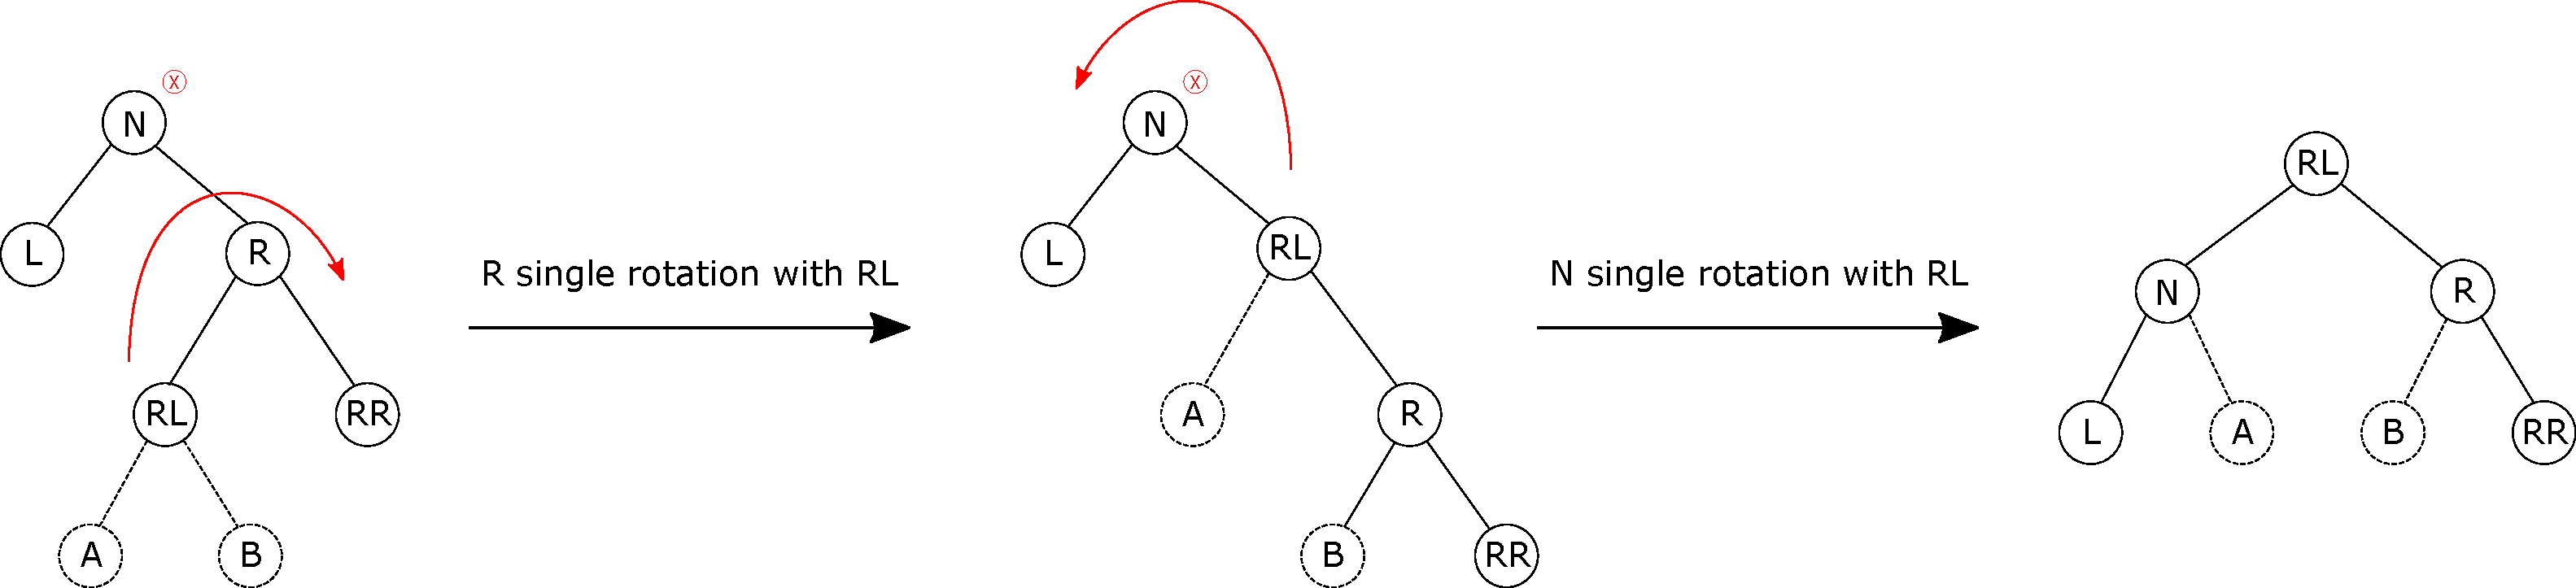
\includegraphics[width=400pt]{./img/AVL-RL-insertion-fix.pdf}
\caption[Figure]{\label{fig:org6fc9e78}
Double rotation to fix AVL-property loss caused by Right-left insertion}
\end{figure}
\subsubsection{Deletion caused unbalance and fix}
\label{sec:org9ec0299}
There are four cases of AVL-property loss by deletion. They are shown in Figure \ref{fig:orgacd8cf6}. The dashed node E indicates where deletion occured. Node E represent the only child of its parent node (doesn't matter if its left or right child). After deleting, its parent's height will be reduced by 1.

\begin{center}
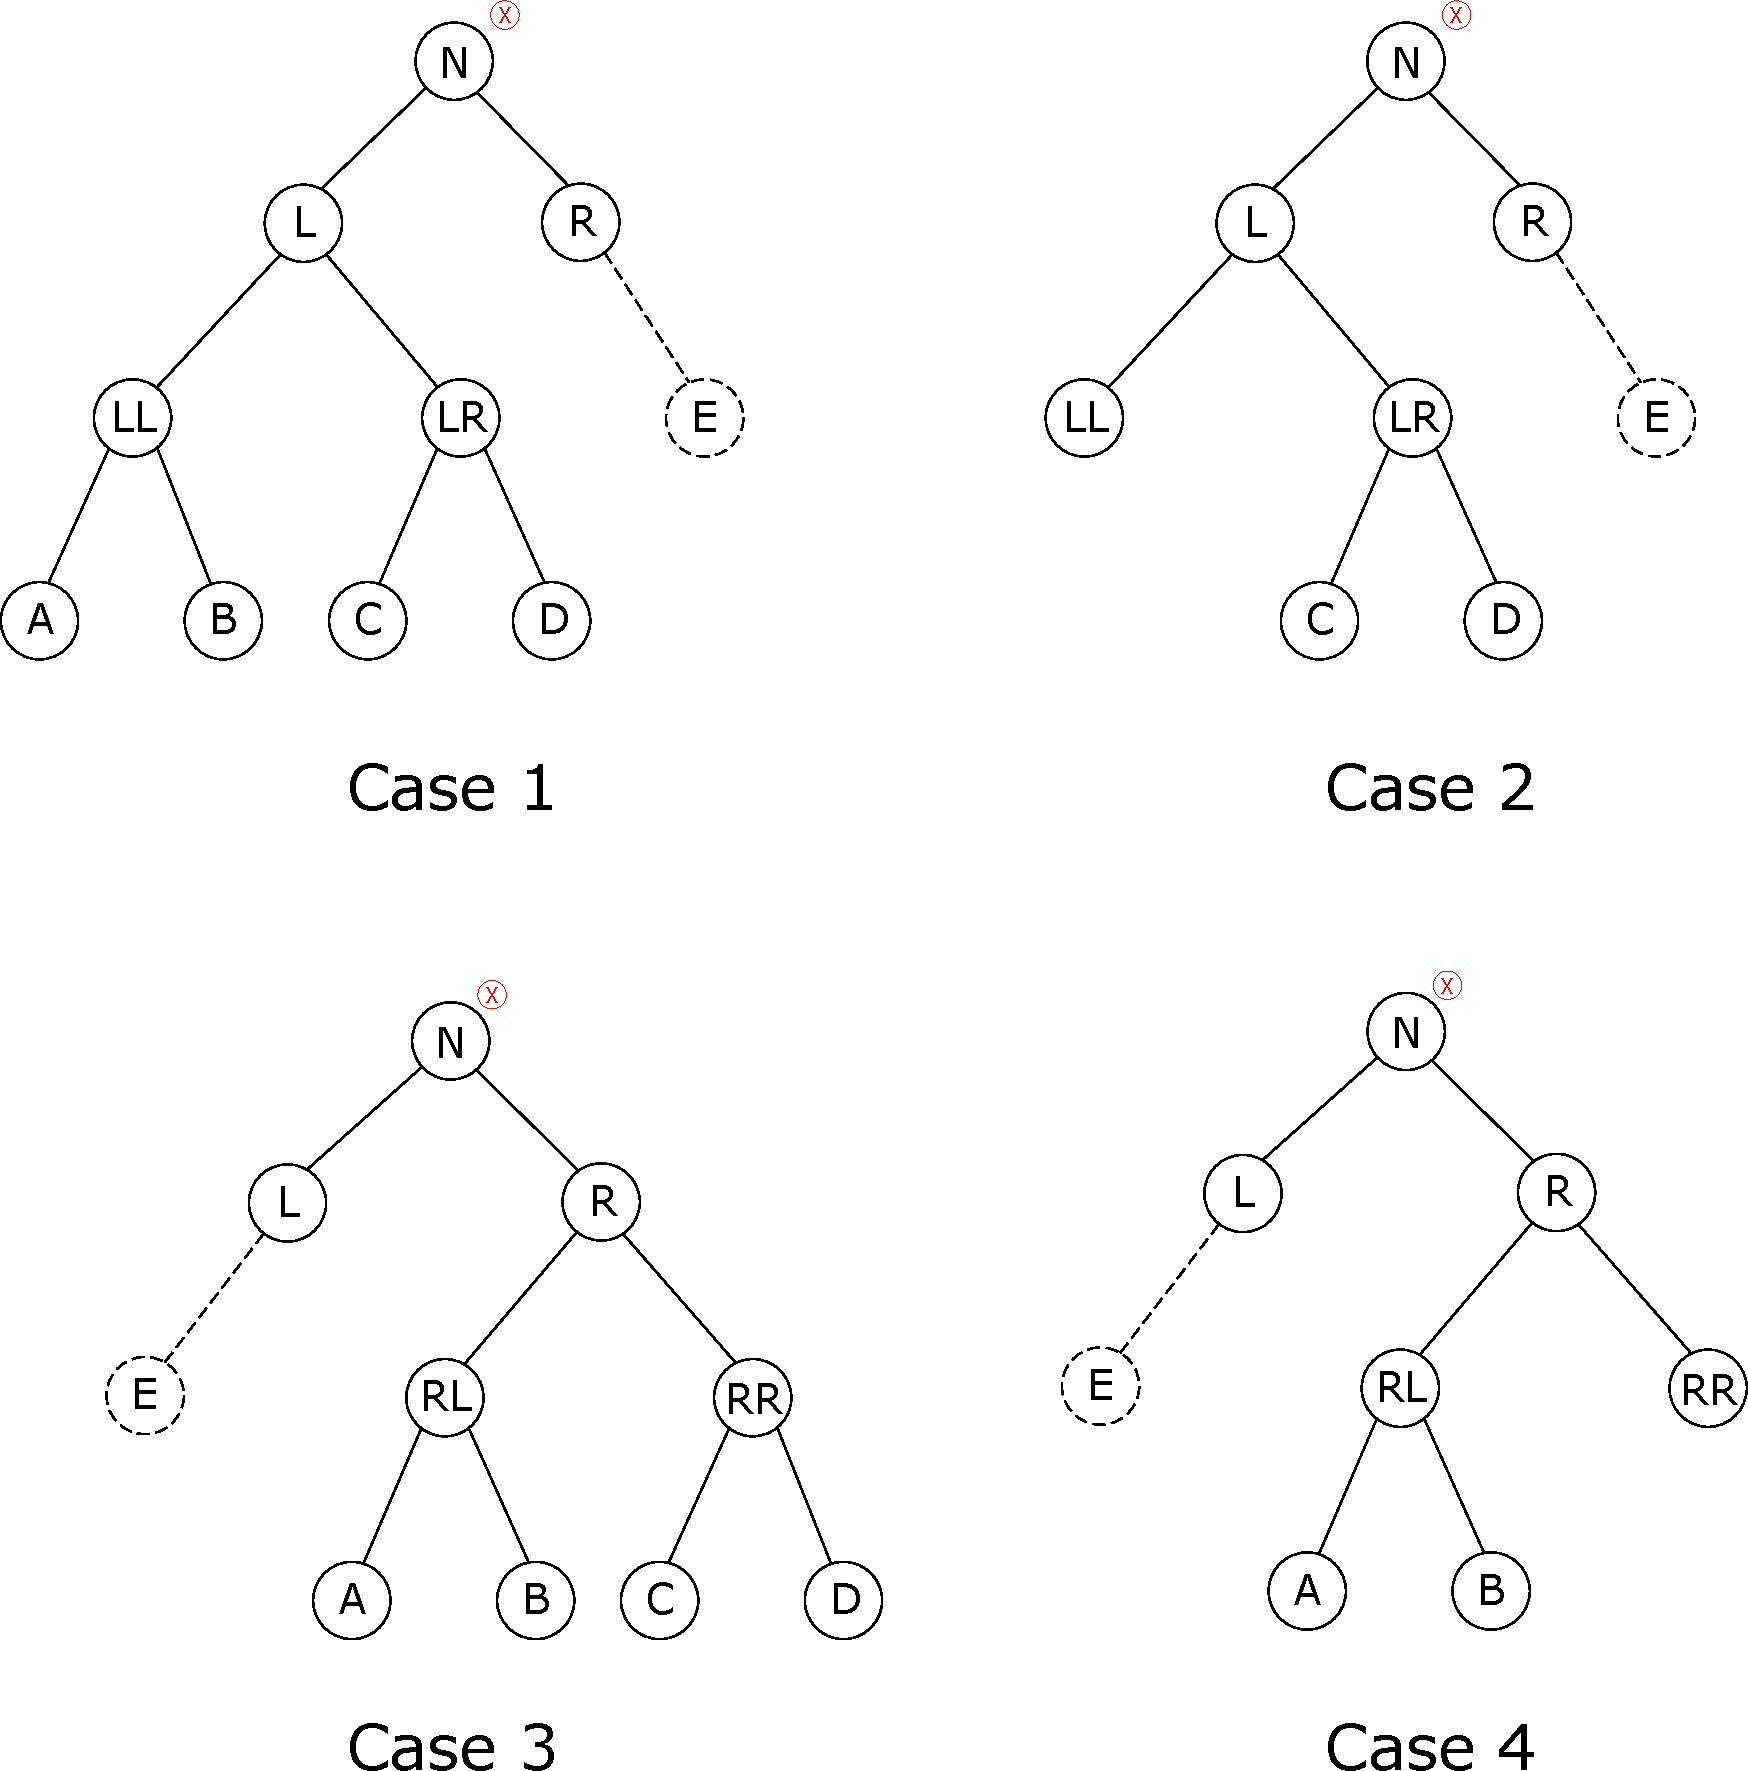
\includegraphics[width=350pt]{./img/AVL-deletion.pdf}
\captionof{figure}{\label{fig:orgacd8cf6}
AVL-property loss by deletion}
\end{center}

To conclude the four cases:

Case 1: \texttt{height(N->left) > height(N->right) + 1}

\texttt{\&\& height(N->left->left) == height(N->left->right)}

Case 2: \texttt{height(N->left) > height(N->right) + 1}

\texttt{\&\& height(N->left->left) < height(N->left->right)}

Case 3: \texttt{height(N->right) > height(N->left) + 1}

\texttt{\&\& height(N->right->right) == height(N->right->left)}

Case 4: \texttt{height(N->right) > height(N->left) + 1}

\texttt{\&\& height(N->right->right) < height(N->right->left)}

Take a closer look, case 1 is similar with LL-insertion case, because they both can be solved with a single rotation of \texttt{N} with \texttt{N->left}. This is because, a single rotation of \texttt{N} with \texttt{N->left} can lower node \texttt{R} one layer, so the height difference between \texttt{R} and bottom nodes will reduced from 2 to 1. Although it can also rise node \texttt{LL} one layer, it will not violate AVL-property since \texttt{height(LL) == height(LR)} before single rotation. After the single rotation, \texttt{heigh(LL)} and \texttt{height(LR)} differ by 1, which is within the requirement. However, this may not be the case when \texttt{height(LL) < height(LR)} initially. Because single rotation will cause \texttt{height(LL) < height(LR) + 1}. This is actually case 2, which is similar with LR-insertion case. They both can be solved with a double rotation: first rotate \texttt{L} with \texttt{L->right}, then rotate \texttt{N} with \texttt{N->left}. The double rotation will rise the height of both node \texttt{C} and \texttt{D}, and will lower the heigh of \texttt{R} by 1 (first single rotation: rise \texttt{D}, lower \texttt{LL}; second single rotation: rise \texttt{LL} and \texttt{C}, lower \texttt{R}).

Using same argument, case 3 is similar with RR-insertion case, and can be fixed by a single rotation of \texttt{N} with \texttt{N->right}. Case 4 is similar with RL-insertion, and can be fixed by a double rotation: first rotate \texttt{R} with \texttt{R->left}, then rotate \texttt{N} with \texttt{N->right}. The fixing for case 2 is the same shown in Figure \ref{fig:org933a468}. The fixing for case 4 is the same shown in Figure \ref{fig:org6fc9e78}. The fixing for case 1 and case 3 is similar with \ref{fig:org8237354}, they are drawn one more time in Figure \ref{fig:org002b49e} and Figure \ref{fig:orga178778}.

\begin{center}
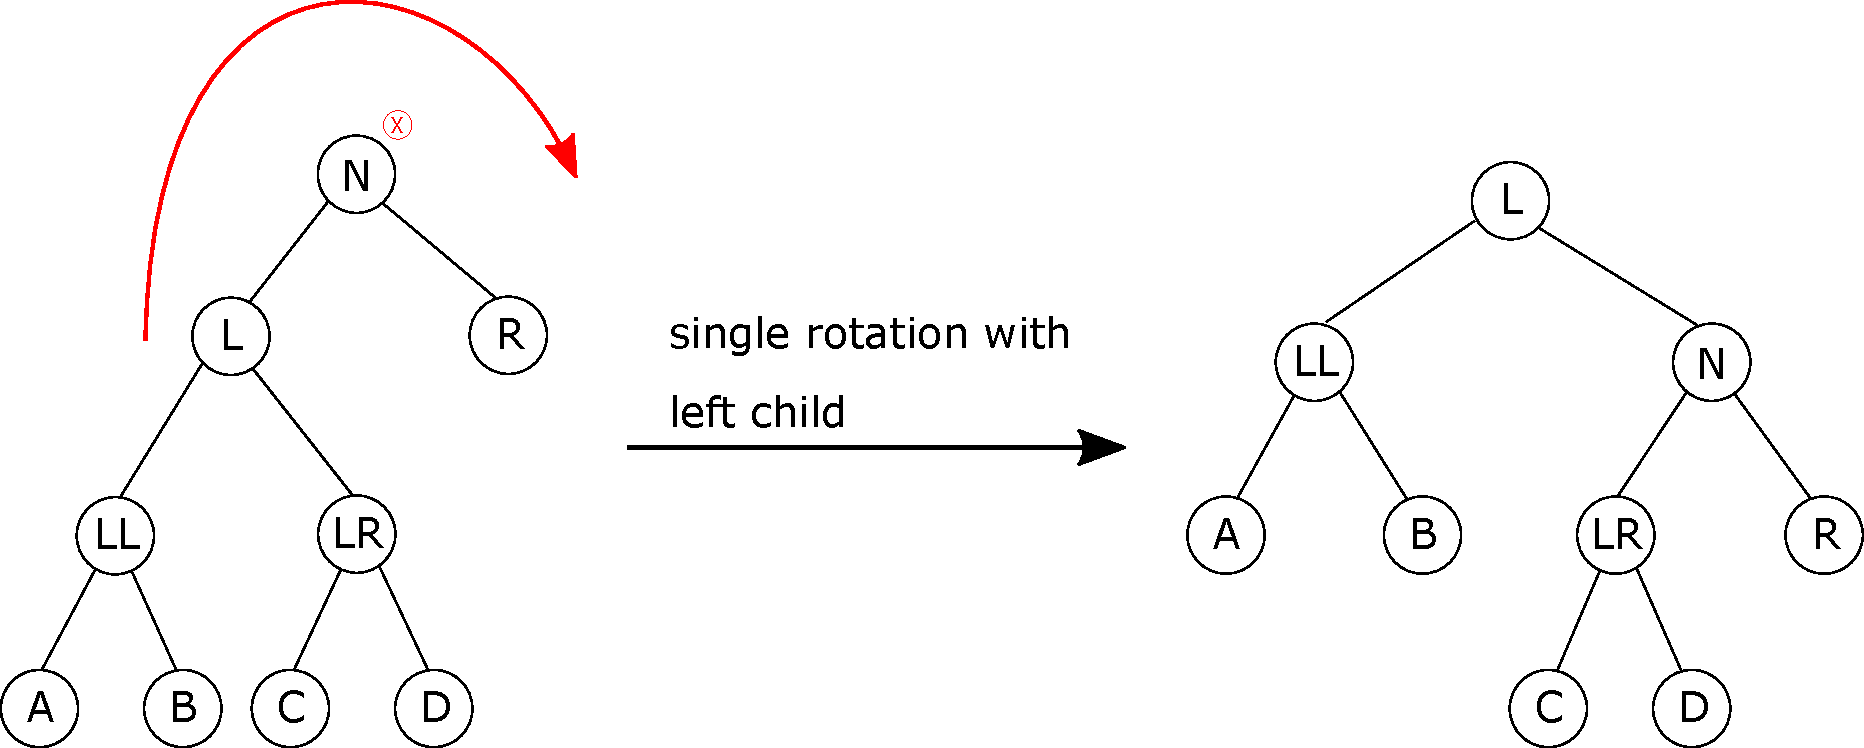
\includegraphics[width=400pt]{./img/AVL-deletion-LL-fix.pdf}
\captionof{figure}{\label{fig:org002b49e}
Balancing AVL tree. When left subtree is too high and its two branches have same height}
\end{center}

\begin{center}
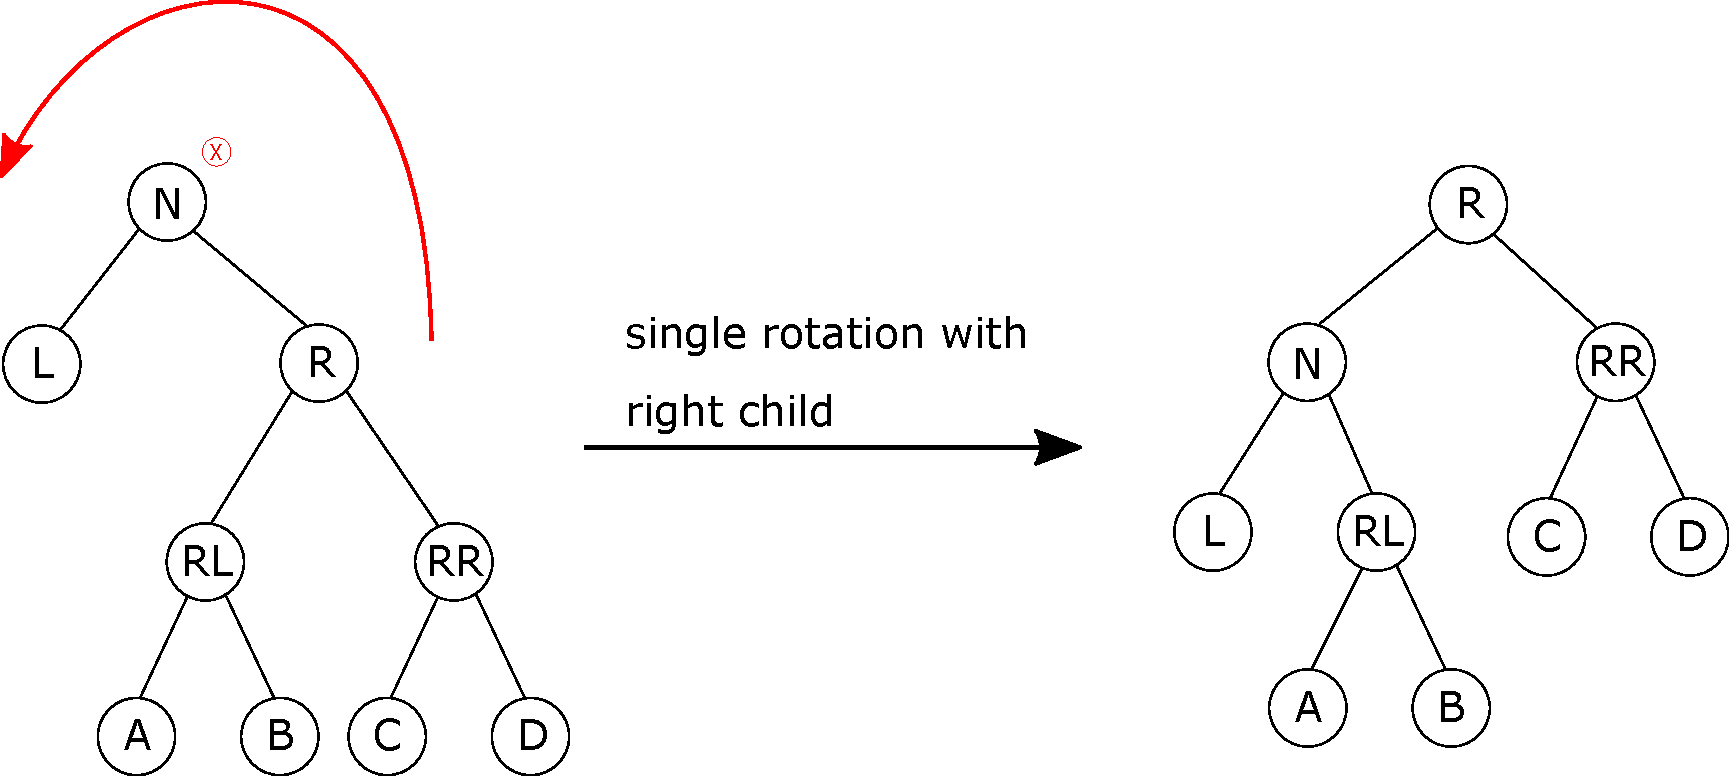
\includegraphics[width=400pt]{./img/AVL-deletion-RR-fix.pdf}
\captionof{figure}{\label{fig:orga178778}
Balancing AVL tree. When right subtree is too high and its two branches have same height}
\end{center}
\subsubsection{Summary}
\label{sec:org98b547e}
From the above analyze, we can see that, if we want to restore the balance for a node \texttt{N}, we first check which side is \textbf{TOO} high (which means the height difference is larger than 1). Then we check if the \textbf{inner} branch of this side is higher than the \textbf{outter} branch, if so, we use double rotation to fix (only double rotation can fix the issue caused by higher inner branch), otherwise, we use single rotation (single rotation is enough to fix issue caused by higher outter branch).

\subsection{Simple Implementation (recursive)}
\label{sec:orgce988fb}
In this section, a simple implementation of AVL tree is discussed. It uses recursive algorithm. Unlike ordinary binary search tree, we have to store extra information in each tree node, which is the height of the node.

\subsubsection{header}
\label{sec:orge0d095f}
We define a nested structure \texttt{AvlNode} inside the \texttt{AVLTree} class. The data member of \texttt{AVLTree} class is just a pointer to \texttt{AvlNode} type, which will be used to hold the root of the AVL tree. We also define a static constant integer variable to indicate the maximum allowed imbalance:
\begin{minted}[breaklines=true,breakanywhere=true,frame=single,framesep=10pt]{c++}
static const int ALLOWED_IMBALANCE = 1;
\end{minted}

Similar with binary tree, we'll use recursive function to implement the AVL tree. It may have slower performance, but is easier to read and understand. What is unique about AVL tree is that we keep it balanced, which is done by the following routines:
\begin{minted}[linenos,firstnumber=1,breaklines=true,breakanywhere=true,frame=single,framesep=10pt]{c++}
void balance(AvlNode* &t); //internal balance routine
void rotateWithLeftChild(AvlNode* &t);
void rotateWithRightChild(AvlNode* &t);
void doubleWithLeftChild(AvlNode* &t);
void doubleWithRightChild(AvlNode* &t);
\end{minted}

We'll discuss each later. The code for the whole header file is as follows:
\begin{minted}[linenos,firstnumber=1,breaklines=true,breakanywhere=true,frame=single,framesep=10pt]{c++}
#pragma once
#include <iostream>
#include <algorithm>

template <typename comparable>
class AVLTree {
private:
  //nested tree node structure
  struct AvlNode { // defined later
  };

private:
  AvlNode* root;
  static const int ALLOWED_IMBALANCE = 1;

private:
  /** private operating functions **/
  ///insert 
  void insert(const comparable& val, AvlNode* & t); //copy
  void insert(comparable&& val, AvlNode* & t); //move

  ///remove
  void remove(const comparable& val, AvlNode* & t);

  ///search 
  AvlNode* findMin(AvlNode* t) const;
  AvlNode* findMax(AvlNode* t) const;
  bool contains(const comparable& val, AvlNode* t) const;

  ///utility
  void makeEmpty(AvlNode* & t);
  void printTree(AvlNode* t, std::ostream& out) const;
  AvlNode* clone(AvlNode* t) const;
  int height(AvlNode* t) const;
  void balance(AvlNode* &t); //internal balance routine
  void rotateWithLeftChild(AvlNode* &t);
  void rotateWithRightChild(AvlNode* &t);
  void doubleWithLeftChild(AvlNode* &t);
  void doubleWithRightChild(AvlNode* &t);

public:
  /** Constructor and destructor **/
  AVLTree(); //zero-parameter default constructor
  AVLTree(const AVLTree& rhs); //copy constructor
  AVLTree(AVLTree&& rhs); //move constructor
  ~AVLTree(); //destructor

  /** Assignment operator **/
  AVLTree& operator=(const AVLTree& rhs); //copy
  AVLTree& operator=(AVLTree&& rhs); //move

  /** Public Search Interface **/
  const comparable& findMin() const;
  const comparable& findMax() const;
  bool contains(const comparable& val) const;

  /** Modification of tree **/
  void makeEmpty();
  void insert(const comparable& val);//copy version
  void insert(comparable&& val);//move version
  void remove(const comparable& val);

  /** Utility **/
  bool isEmpty() const;
  void printTree(std::ostream& out = std::cout) const;

};

//include implementation here 
#include "avl.hpp"
\end{minted}

\subsubsection{AVL node structure}
\label{sec:org4fd27b1}
The node of AVL tree uses a variable to hold the height information of the node. During construction, the default height is 0, the constructor accepts an integer to pass it to the height member, setting the height during construction. Code:
\begin{minted}[linenos,firstnumber=1,breaklines=true,breakanywhere=true,frame=single,framesep=10pt]{c++}
struct AvlNode {
  comparable element;//data stored in the node, and it is comparable (at least one comparable routine is defined for this type)
  AvlNode* left;
  AvlNode* right;
  int height; //store the height of this node

  ///constructor
  //copy
  AvlNode(const comparable& val = val{}, AvlNode* lt = nullptr, AvlNode* rt = nullptr, int h = 0) : element {val}, left {lt}, right {rt}, height {h} {}
  //move
  AvlNode(comparable&& val = val{}, AvlNode* lt = nullptr, AvlNode* rt = nullptr, int h = 0) : element {std::move(val)}, left {lt}, right {rt}, height {h} {}
};
\end{minted}
\subsubsection{\texttt{zero parameter constructor}}
\label{sec:orgc02b40a}
\texttt{root} will be initialized to \texttt{nullptr}. Code:
\begin{minted}[linenos,firstnumber=1,breaklines=true,breakanywhere=true,frame=single,framesep=10pt]{c++}
template <typename comparable>
AVLTree<comparable>::AVLTree() : root {nullptr} {}
\end{minted}
\subsubsection{\texttt{copy constructor}}
\label{sec:org6eaf9f0}
\texttt{clone()} routine will be used, similar with binary search tree. Code:
\begin{minted}[linenos,firstnumber=1,breaklines=true,breakanywhere=true,frame=single,framesep=10pt]{c++}
template <typename comparable>
AVLTree<comparable>::AVLTree(const AVLTree& rhs) {
  root = clone(rhs.root);
}
\end{minted}
\subsubsection{\texttt{move constructor}}
\label{sec:org72400a7}
Same as binary search tree, code:
\begin{minted}[linenos,firstnumber=1,breaklines=true,breakanywhere=true,frame=single,framesep=10pt]{c++}
template <typename comparable>
AVLTree<comparable>::AVLTree(AVLTree&& rhs) {
  root = rhs.root;
  rhs.root = nullptr;
}
\end{minted}
\subsubsection{\texttt{destructor}}
\label{sec:orgc6fad5f}
Same as binary search tree, code:
\begin{minted}[breaklines=true,breakanywhere=true,frame=single,framesep=10pt]{c++}
template <typename comparable>
AVLTree<comparable>::~AVLTree() {
  makeEmpty();
}
\end{minted}
\subsubsection{\texttt{copy assignment operator}}
\label{sec:org14bc0f6}
Same as binary search tree, code:
\begin{minted}[linenos,firstnumber=1,breaklines=true,breakanywhere=true,frame=single,framesep=10pt]{c++}
AVLTree<comparable>& AVLTree<comparable>::operator=(const AVLTree& rhs) {
  root = clone(rhs.root);
  return *this;
}
\end{minted}
\subsubsection{\texttt{move assignment operator}}
\label{sec:org39d672b}
Same as binary search tree, code:
\begin{minted}[linenos,firstnumber=1,breaklines=true,breakanywhere=true,frame=single,framesep=10pt]{c++}
template <typename comparable>
AVLTree<comparable>& AVLTree<comparable>::operator=(AVLTree&& rhs) {
  root = rhs.root;
  rhs.root = nullptr;
  return *this;
}
\end{minted}
\subsubsection{public \texttt{findMin()}}
\label{sec:org23cf28e}
Same as binary search tree, code:
\begin{minted}[linenos,firstnumber=1,breaklines=true,breakanywhere=true,frame=single,framesep=10pt]{c++}
template <typename comparable>
const comparable& AVLTree<comparable>::findMin() const {
  return (findMin(root))->element;
}
\end{minted}
\subsubsection{public \texttt{findMax()}}
\label{sec:org38ca6a4}
Same as binary search tree, code:
\begin{minted}[linenos,firstnumber=1,breaklines=true,breakanywhere=true,frame=single,framesep=10pt]{c++}
template <typename comparable>
const comparable& AVLTree<comparable>::findMax() const {
  return (findMax(root))->element;
}
\end{minted}
\subsubsection{public \texttt{contains()}}
\label{sec:orgbfcb98d}
\begin{minted}[linenos,firstnumber=1,breaklines=true,breakanywhere=true,frame=single,framesep=10pt]{c++}
template <typename comparable>
bool AVLTree<comparable>::contains(const comparable& val) const {
  return contains(val, root);
}
\end{minted}
\subsubsection{public \texttt{makeEmpty()}}
\label{sec:orgcf45433}
\begin{minted}[linenos,firstnumber=1,breaklines=true,breakanywhere=true,frame=single,framesep=10pt]{c++}
template <typename comparable>
void AVLTree<comparable>::makeEmpty() {
  makeEmpty(root);
}
\end{minted}
\subsubsection{public \texttt{insert()}}
\label{sec:orgf41d0c2}
Copy version:
\begin{minted}[linenos,firstnumber=1,breaklines=true,breakanywhere=true,frame=single,framesep=10pt]{c++}
template <typename comparable>
void AVLTree<comparable>::insert(const comparable& val) {
  insert(val, root);
}
\end{minted}
\subsubsection{public \texttt{remove()}}
\label{sec:org103d783}
\begin{minted}[linenos,firstnumber=1,breaklines=true,breakanywhere=true,frame=single,framesep=10pt]{c++}
template <typename comparable>
void AVLTree<comparable>::remove(const comparable& val) {
  remove(val, root);
}
\end{minted}
\subsubsection{public \texttt{isEmpty()}}
\label{sec:orgf723b97}
\begin{minted}[linenos,firstnumber=1,breaklines=true,breakanywhere=true,frame=single,framesep=10pt]{c++}
template <typename comparable>
bool AVLTree<comparable>::isEmpty() const {
  if (root == nullptr)
    return true;
  else 
    return false;
}
\end{minted}
\subsubsection{public \texttt{printTree()}}
\label{sec:orga9e7e11}
\begin{minted}[linenos,firstnumber=1,breaklines=true,breakanywhere=true,frame=single,framesep=10pt]{c++}
template <typename comparable>
void AVLTree<comparable>::printTree(std::ostream& out) const {
  printTree(root, out);
}
\end{minted}
\subsubsection{\texttt{insert()}}
\label{sec:org3fa24a5}
This function accepts a pointer to \texttt{AvlNode} type \texttt{t} and a \texttt{AvlNode} type variable \texttt{val}. It will try to insert \texttt{val} into subtree started with \texttt{t}. The inserting process is the same as binary search tree. After inserting, \texttt{balance()} will be called to:
\begin{enumerate}
\item check if balance of \texttt{t} is violated
\item balance the tree if necessary
\item update the height of the node pointed by \texttt{t}
\end{enumerate}

Code (copy version):
\begin{minted}[linenos,firstnumber=1,breaklines=true,breakanywhere=true,frame=single,framesep=10pt]{c++}
template <typename comparable>
void AVLTree<comparable>::insert(const comparable& val, AvlNode* & t) {  
  //base case1: t is pointing to nullptr
  if (t == nullptr) {
    t = new AvlNode{val}; //this step will modify t, so pass the pointer by reference is necessary
  }

  //determine which branch to insert 
  //when item being inserted is the same as t->element, do nothing (don't insert)
  else if (val < t->element)
    insert(val, t->left);
  else if (val > t->element)
    insert(val, t->right);

  balance(t);
}
\end{minted}
\subsubsection{\texttt{remove()}}
\label{sec:orgea98de3}
Similar with \texttt{insert()}, \texttt{balance(t)} will be called after removing the node (which may cause potential height change). Code:
\begin{minted}[linenos,firstnumber=1,breaklines=true,breakanywhere=true,frame=single,framesep=10pt]{c++}
template <typename comparable>
void AVLTree<comparable>::remove(const comparable& val, AvlNode* & t) {
  //base case 1: t is pointing to nullptr, no match
  if (t == nullptr)
    return;

  //base case 2: t is pointing to the target node
  if (t->element == val) {
    //find the left most spot of t->right, and attach t->left to it
    if (t->right == nullptr) {
      t->right = t->left;
    }

    else {
      AvlNode* left_leaf_ptr = t->right;
      while (left_leaf_ptr -> left != nullptr)
	left_leaf_ptr = left_leaf_ptr -> left;
      //after the above loop, left_leaf_ptr is pointing to the left most leaf of t->right, attach t->left to the left subtree of this leaf
      left_leaf_ptr -> left = t->left;
    }

    //keep record of the address of current t->right
    AvlNode* temp = t->right;
    //reclaim memory 
    delete t;
    //re-connect tree node 
    t = temp;

  }

  //t is not pointing to the target node
  else if (t->element > val) 
    remove(val, t->left);
  else if (t->element < val)
    remove(val, t->right);

  //balance the node to correct height-change induced un-balancing situation
  balance(t);  
}
\end{minted}
\subsubsection{\texttt{findMin()}}
\label{sec:orgdb72e37}
\begin{minted}[linenos,firstnumber=1,breaklines=true,breakanywhere=true,frame=single,framesep=10pt]{c++}
template <typename comparable>
typename AVLTree<comparable>::AvlNode* AVLTree<comparable>::findMin(AvlNode* t) const {
  if (t == nullptr)
    return t;

  while (t->left != nullptr)
    t = t->left;
  //after the above loop, t is not pointing to left-most leaf
  return t;  
}
\end{minted}
\subsubsection{\texttt{findMax()}}
\label{sec:org02be89c}
\begin{minted}[linenos,firstnumber=1,breaklines=true,breakanywhere=true,frame=single,framesep=10pt]{c++}
template <typename comparable>
typename AVLTree<comparable>::AvlNode* AVLTree<comparable>::findMax(AvlNode* t) const {
  if (t == nullptr)
    return t;

  while (t->right != nullptr)
    t = t->right;
  //after the above loop, t is not pointing to right-most leaf
  return t;   
}
\end{minted}
\subsubsection{\texttt{contains()}}
\label{sec:org5620db0}
\begin{minted}[linenos,firstnumber=1,breaklines=true,breakanywhere=true,frame=single,framesep=10pt]{c++}
template <typename comparable>
bool AVLTree<comparable>::contains(const comparable& val, AvlNode* t) const {
  //base case: t == nullptr, no match found
  if (t == nullptr)
    return false;

  //base case2: t->element == val
  if (t->element == val)
    return true;

  //try to find val in t's children
  if (t->element > val)
    return contains(val, t->left);
  else 
    return contains(val, t->right);
}
\end{minted}
\subsubsection{\texttt{makeEmpty()}}
\label{sec:org1066456}
\begin{minted}[linenos,firstnumber=1,breaklines=true,breakanywhere=true,frame=single,framesep=10pt]{c++}
template <typename comparable>
void AVLTree<comparable>::makeEmpty(AvlNode* & t) {
  //base case 
  if (t == nullptr)
    return;

  //begin makeEmpty
  makeEmpty(t->left);
  makeEmpty(t->right);
  delete t;
  t = nullptr;
}
\end{minted}
\subsubsection{\texttt{printTree()}}
\label{sec:orgdb1c5ec}
\begin{minted}[linenos,firstnumber=1,breaklines=true,breakanywhere=true,frame=single,framesep=10pt]{c++}
template <typename comparable>
void AVLTree<comparable>::printTree(AvlNode* t, std::ostream& out) const {
  //base case 
  if (t == nullptr)
    return;

  //print the tree in inorder traversal
  printTree(t->left, out);
  out << t->element << ' ';
  printTree(t->right, out);
}
\end{minted}
\subsubsection{\texttt{clone()}}
\label{sec:org2aee1cd}
\begin{minted}[linenos,firstnumber=1,breaklines=true,breakanywhere=true,frame=single,framesep=10pt]{c++}
template <typename comparable>
typename AVLTree<comparable>::AvlNode* AVLTree<comparable>::clone(AvlNode* t) const {
  /** pay attention that what you clone is an AvlNode! **/
  //base case 
  if (t == nullptr)
    return t;

  //clone 
  return new AvlNode{t->element, clone(t->left), clone(t->right)};
}
\end{minted}
\subsubsection{\texttt{rotateWithLeftChild()}}
\label{sec:orga353f6e}
This function accepts a pointer to \texttt{AvlNode} type: \texttt{t}, and the AVL property of \texttt{*t} is violated. It will fix it by performing rotation of \texttt{t} with \texttt{t->left}. The process is illustrated in Figure \ref{fig:org8237354}. Pay attention that, besides rotating, you have to also update the height of each altered node, i.e. \texttt{t} and \texttt{t->left}. Then you reconnect \texttt{t->left} back to tree. \texttt{std::max()} is used to return the larger height of a node. And the node's height is obtained by calling \texttt{height()} routine.
Code:
\begin{minted}[linenos,firstnumber=1,breaklines=true,breakanywhere=true,frame=single,framesep=10pt]{c++}
template <typename comparable>
void AVLTree<comparable>::rotateWithLeftChild(AvlNode* &t) {
  // rotate
  auto temp = t->left;
  t->left = temp->right;
  temp->right = t;

  // update height
  t->height = std::max(height(t->left), height(t->right)) + 1;
  temp->height = std::max(height(temp->left), t->height) + 1;

  // reconnect temp to where t was
  t = temp;
}
\end{minted}
\subsubsection{\texttt{rotateWithRightChild()}}
\label{sec:orgd0d404d}
This is similar with \texttt{rotateWithLeftChild()}. Code:
\begin{minted}[linenos,firstnumber=1,breaklines=true,breakanywhere=true,frame=single,framesep=10pt]{c++}
template <typename comparable>
void AVLTree<comparable>::rotateWithRightChild(AvlNode* &t) {
  AvlNode* temp = t->right;
  t->right = temp->left;
  temp->left = t;

  //update height information
  t->height = std::max(height(t->left), height(t->right)) + 1;
  temp->height = std::max(height(temp->right), t->height) + 1;

  //connect temp to where t was
  t = temp;
}
\end{minted}
\subsubsection{\texttt{doubleWithLeftChild()}}
\label{sec:org6075a56}
This function will perform a double rotation. The process is illustrated in \ref{fig:org933a468}. Notice that you can call single rotation routine to rotate (height change is also taken care of by single rotation routine). Code:
\begin{minted}[linenos,firstnumber=1,breaklines=true,breakanywhere=true,frame=single,framesep=10pt]{c++}
template <typename comparable>
void AVLTree<comparable>::doubleWithLeftChild(AvlNode* &t) {
  rotateWithRightChild(t->left);
  rotateWithLeftChild(t);
}
\end{minted}
\subsubsection{\texttt{doubleWithRightChild()}}
\label{sec:orgbd01de2}
This function will perform a double rotation. The process is illustrated in \ref{fig:org6fc9e78}. Notice that you can call single rotation routine to rotate (height change is also taken care of by single rotation routine). Code:
\begin{minted}[linenos,firstnumber=1,breaklines=true,breakanywhere=true,frame=single,framesep=10pt]{c++}
template <typename comparable>
void AVLTree<comparable>::doubleWithRightChild(AvlNode* &t) {
  rotateWithLeftChild(t->right);
  rotateWithRightChild(t);
}
\end{minted}
\subsubsection{\texttt{balance()}}
\label{sec:org6a88c44}
This function accepts a pointer to \texttt{AvlNode} type: \texttt{t}. It will first check if the AVL property is violated, if so, it will try to fix it using the four rotation routines. The algorithm is based on previous analysis. Pay attention that you sould update the height of the current node.
\begin{minted}[linenos,firstnumber=1,breaklines=true,breakanywhere=true,frame=single,framesep=10pt]{c++}
template <typename comparable>
void AVLTree<comparable>::balance(AvlNode* &t) {
  //check nullptr
  if (t == nullptr)
    return;

  //check which branch inserted
  if (height(t->left) > height(t->right) + ALLOWED_IMBALANCE) {// left subtree of t is higher
    if (height(t->left->left) < height(t->left->right)) //LR case
      doubleWithLeftChild(t);
    else //LL case
      rotateWithLeftChild(t);
  }

  else if (height(t->right) > height(t->left) + ALLOWED_IMBALANCE) {//right subtree of t is higher 
    if (height(t->right->right) < height(t->right->left)) //RL case
      doubleWithRightChild(t);
    else //RR case
      rotateWithRightChild(t);
  }

  //update height of the current node
  t->height = std::max(height(t->left), height(t->right)) + 1;
}
\end{minted}
\subsubsection{\texttt{height()}}
\label{sec:org206fd90}
By default, the height of an empty AVL tree is -1. Code:
\begin{minted}[linenos,firstnumber=1,breaklines=true,breakanywhere=true,frame=single,framesep=10pt]{c++}
template <typename comparable>
int AVLTree<comparable>::height(AvlNode* t) const {
  return t == nullptr ? -1 : t->height;
}
\end{minted}

\section{Red Black Tree}
\label{sec:orgce3dfc5}
\subsection{General Idea}
\label{sec:org9f753fa}
\chapter{Hash Table}
\label{sec:org454023a}
Hash table ADT is a way of organizing data. It only allows a subset of operations of binary search tree. However, Hash table has higher efficiency on these supported operations than binary search tree. For example, Hash table can perform insertion, deletion and find in \textbf{CONSTANT} average time.

One point should be made clear that, Hash table does not support operation that requires ordering information.
\section{General Idea}
\label{sec:orgcc49382}
\subsection{Key}
\label{sec:org6d235ef}

A key is part of the data item that is used to perform searching by some methods. We search the \textbf{key} and find the match item, then we declare that we have found the item.
\subsection{Vector/Array}
\label{sec:org17c009f}

The ideal Hash table data structure is merely an array (which has a fixed size) containing our data items. Imagine we have a bunch of data items to be put into an array. In order to achieve constant time access, we may think design a certain rule of how to put items into the array. This rule can be a mapping from a specific key to the actual index in that array. We can define some part of our data item as the \textbf{KEY} to be used to get the index through the mapping. So, for each data item, we can find out where we should put it in the array. And we can also find out the existence of a specific data item by using the corresponding key in constant time.

Basically, hash table is an array that manages the position of data items by their key, rather than their sequence of inserting into the array. Figure \ref{fig:orgd23e753} shows the comparison between array storage and hash table storage.

\begin{center}
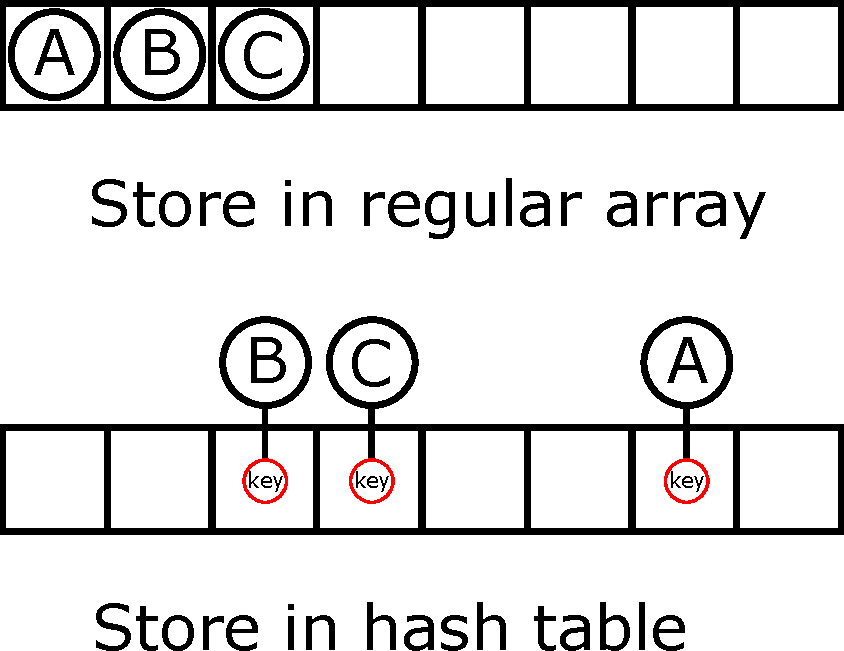
\includegraphics[width=200pt]{./img/Hash-hashtable-illustration.pdf}
\captionof{figure}{\label{fig:orgd23e753}
Comparison between array storage and hash table storage}
\end{center}


\section{Hash Function}
\label{sec:org244f4d6}

The mapping we mentioned above is called a hash function. Ideally, a hash function should:
\begin{enumerate}
\item be simple to compute
\item can ensure that any two distinct keys get different index value
\end{enumerate}

The fact that there are a finite number of cells and a virtually inexhaustible supply of keys makes 2 impossible. In practical, we try our best to achieve it. By that, it means seek a hash function that distributes the keys as even as possible among the slots of the array.

If the input keys are integers already, simpliy choose \texttt{hash(key)} as \texttt{key \% array.size()}. If \texttt{array.size()} is a prime number, this hash function can distribute the keys evenly.

If the input keys are not integer, our strategy contains two steps:
\begin{enumerate}
\item convert the key into integer \texttt{i}
\item calculate \texttt{i \% array.size()} to get the index
\end{enumerate}

In practice, the function that fullfills step 1 is called hash function. The second step is trival.

\subsection{Hash Function Object}
\label{sec:orgf37d24f}
We have to design the details of how hash function convert a non-integer data type into integer value. For example, to convert a string object to integer value. We can just directly write a function that accepts \texttt{std::string} and returns \texttt{size\_t}:
\begin{minted}[linenos,firstnumber=1,breaklines=true,breakanywhere=true,frame=single,framesep=10pt]{c++}
size_t hash(const std::string& key) {
  size_t hashVal = 0;
  for (char ch:key)
    hashVal = 37 * hashVal + ch;
  return hashVal;
}
\end{minted}

To do this job in a more generic way, we can define a hash function object. A function object (also called a functor) is a class object with \texttt{operator()} defined. This operator is called function call operator, which can make the object be used like a function. For example:
\begin{minted}[linenos,firstnumber=1,breaklines=true,breakanywhere=true,frame=single,framesep=10pt]{c++}
class Add {
public:
  int operator()(int a, int b) {
    return (a + b);
  }
};
\end{minted}

In the above code, we defined a class named \texttt{Add}. It has only one public member function \texttt{operator()}, which accepts two integer parameters \texttt{a} and \texttt{b}. It will return the result of \texttt{a + b}. To use it, we can:
\begin{minted}[linenos,firstnumber=1,breaklines=true,breakanywhere=true,frame=single,framesep=10pt]{c++}
Add addition; // declare an object
std::cout << "1 + 1 is: " << addition(1, 1); // operator() is called
\end{minted}

We can also write a template:
\begin{minted}[linenos,firstnumber=1,breaklines=true,breakanywhere=true,frame=single,framesep=10pt]{c++}
template <class T>
class Add {
public:
  T operator()(T a, T b) {
    return (a + b);
  }
};
\end{minted}

To use it:
\begin{minted}[linenos,firstnumber=1,breaklines=true,breakanywhere=true,frame=single,framesep=10pt]{c++}
Add addition<int>; // declare an object
std::cout << "1 + 1 is: " << addition(1, 1); // operator() is called
\end{minted}

You can also write a \textbf{specialization} of the template for a spefic type. For example:
\begin{minted}[linenos,firstnumber=1,breaklines=true,breakanywhere=true,frame=single,framesep=10pt]{c++}
// for generic type T
template <class T>
class Add {
public:
  T operator()(T a, T b) {
    return (a + b);
  }
};

// for string type
template<> // you'll provide the specific type below
class Add<std::string> { // provide type here
public:
  int operator()(std::string a, std::string b) {
    return (std::stoi(a) + std::stoi(b));
  }
};
\end{minted}

This is called template specialization. You write the implementation of the class using one specific type. Pay attention that, if all the template typename is designated, it will be implemented during compile.

Back to our hash function object. We can first declare an empty template and write template specialization for different types of key we want to convert to integer. For example, in the following code, hash function for \texttt{std::string} and \texttt{double} are defined.
\begin{minted}[linenos,firstnumber=1,breaklines=true,breakanywhere=true,frame=single,framesep=10pt]{c++}
#pragma once
#include <string>
//an empty function object template
template <typename Key>
class hash {
public:
  size_t operator()(const Key& k) const;
};

//a specialization of hash function, which accepts a string and return the converted integer value 
template<>
class hash<std::string> {
public:
  size_t operator()(const std::string& k) const {
    size_t hashVal = 0;
    for(char ch:k)
      hashVal = 37 * hashVal + ch;
    return hashVal;
  }
};

//a specialization of hash function, which accepts a double and return the converted hash value (this is only for test purpose, so the hash function is bad)
template<>
class hash<double> {
public:
  size_t operator()(double k) const {
    if (double < 0)
      double = 0 - double;

    size_t hashVal{static_cast<size_t>(k)}; //requires narrowing conversion

    return hashVal;
  }
};
\end{minted}

The above code is wrapped in a header file (this header file is considered to store the hash function). When using hash table, we may want to use it to hold user-defined data type, like an object of user-defined class. It is your duty to provide usable hash function specialization that can convert the user-defined class into integer value. Generally, this specialization of hash function should be inside the declaration file of the class that is going to be put into hash table (so as long as you included the class, you can use it in hash table container). The keyword of the name of hash function is just that: \texttt{hash()}.

For example, suppose I have a class named \texttt{Employee}. It has following private data member:
\begin{minted}[breaklines=true,breakanywhere=true,frame=single,framesep=10pt]{c++}
std::string name;
double salary;
\end{minted}

Now I want to use \texttt{name} as the key to generate the hash-value of an employee object. So I have to put following template specialization of hash function into the header file of \texttt{Employee} class (employee.h):
\begin{minted}[linenos,firstnumber=1,breaklines=true,breakanywhere=true,frame=single,framesep=10pt]{c++}
template<>
class hash<Employee> {
public:
  size_t operator()(const Employee& item) {
    static hash<std::string> hf;
    return hf(item.getName()); //this line makes it clear that, the returned value of item.getName() will be used as key of item, which is a string
  }
};
\end{minted}

Notice that, inside the implementation, I created an object of \texttt{hash<std::string>} type. This is to utilize the hash function that accepts a \texttt{std::string} type, an example of using hash function for pre-defined types to build our own hash function.

The keyword \texttt{static} is just tell computer that only one copy of the \texttt{hash<std::string>} object is needed in case of multiple calling of \texttt{hash<Employee>::operator()}. \texttt{getName()} is the routine in \texttt{Employee} class that returns \texttt{name}.


\subsection{Hash Function in C++ STL}
\label{sec:org05d53ea}

Designing a good hash function is usually very hard in practical, and is usually done by mathematicians working in related field. In C++ STL, we have predefined hash function for primitive types as well as types predefined in C++ STL (like \texttt{std::string}). To use it, you have to:
\begin{minted}[breaklines=true,breakanywhere=true,frame=single,framesep=10pt]{c++}
#include <functional>
\end{minted}

Hash function for \texttt{std::string} object is defined in \texttt{<string>} header file. Pay attention that you still need to write the specific version of hash function that accepts your own user-defined class (by giving a template specialization in the user-defined class).

Using the same example in the previous section, the following code shows how to implement the hash function specialization for \texttt{Employee} class using C++ STL provided hash function instead:
\begin{minted}[linenos,firstnumber=1,breaklines=true,breakanywhere=true,frame=single,framesep=10pt]{c++}
#include <string> // enable C++ STL hash function for string
template<>
class hash<Employee> {
public:
  size_t operator()(const Employee& item) {
    static std::hash<std::string> hf;
    return hf(item.getName()); //this line makes it clear that, the returned value of item.getName() will be used as key of item, which is a string
  }
};
\end{minted}

\section{Collision Management}
\label{sec:orgb1e302b}
Collision happens when inserting an element, it hashes to the same value as a previously inserted element. The probability of collision increases as the hash table gets full. There are various ways to manage collision, in this section following will be introduced briefly:
\begin{itemize}
\item separate chaining
\item probing
\begin{itemize}
\item linear probing
\item quadratic probing
\end{itemize}
\item double hashing
\end{itemize}

\subsection{Separate chaining}
\label{sec:org549d1fd}

This strategy will keep a doubly-linked list (\texttt{std::list}) of all elements that hash to the same value. The hash table array will not store data element directly, it keeps track of a doubly linked list of data element in the array instead. If collision happens, data element hashes to the same index value will be pushed into the list. Actually, any containers can be used beside linked list, for example: binary tree, another hash table.

Load factor \(\lambda\) is defined as:
\[
\lambda = \frac {\text{total number of items in hash table}} {\text{hash table size}} = \frac {\text{total number of items}} {\text{number of linked list}}
\]
so, load factor is also the average length of the linked list. A successful search requires about \(1 + \frac {\lambda} {2}\) links to be traversed. \(\frac {\lambda} {2}\) corresponds to expected number of other elements traversed before we find match, 1 corresponds to the matched element.

To reduce the chance of collision, we want to keep \(\lambda\) low. When \(\lambda \approx 1\), we may want to resize the hash table. When copying old items into new array, we have to use hash function to re-calculate the appropriate index for each of the item. This process is called rehash.

\subsection{Probing}
\label{sec:org84681a4}
In this strategy, if an element is hased to a slot that is already occupied, we try alternative slots until an empty cell is found. The operation of trying to find an empty alternative slot is called probing. So, how to calculate these ``alternative'' index value if the first hashed value is already occupied?

We list the alternative indexes as:
\[
h_0(x), h_1(x), h_2(x), \cdots
\]
where
\[
h_i(x) = [hash(x) + f(i)] \bmod \text {tableSize}
\]
with \(f(0) = 0\).

The function \(f(i)\) is called the collision resolution strategy. A hash table doesn't use separate chaining requires a larger table than those use. Generally, \(\lambda\) should be kept below 0.5.

\subsubsection{Linear probing}
\label{sec:org6004f57}
Linear probing is to use linear function of \(i\), typically \(f(i) = i\). Basically, if one spot is occupied, we move to the adjacent spot. Repeat this process until we find an empty spot. As long as the table is big enough, an empty spot can clways be found. However, the time to do so cen get quite large (for both insertion and searching). Another issue is blocks of occupied slots start forming quickly, which is known as primary clustering. 

\subsubsection{Quadritic probing}
\label{sec:org9cd057e}
Quadritic probing is to use quadratic function of \(i\), typically \(f(i) = i^2\). If the table size is prime number, there is no guarantee of finding an empty cell once the table gets more than half full. This is because at most half of the table can be used as alternative location to resolve collisions for objects that hash to same index value in the begining (\(h_o(x)\)). Formally, we have the following theorem:

\textbf{THEOREM}
\begin{quote}
If quadratic probing is used, and the table size is prime, then a new element can \textbf{always} be inserted if the table is at most half empty
\end{quote}

\textbf{PROOF}

Intuitively, we can imagine why we are facing this problem: even if the table is not full, we still can't insert an item. Unlike linear probing, quadratic probing is not probing empty slot \textbf{one by one}. For linear probing, as long as there is empty cell, we can always get there. For quadratic probing, we are skipping some empty slots. In fact, when inserting an element, we first calculate \(h_0(x)\), then all the possible \(h_i(x)\) can be calculated:
\begin{align*}
h_0(x) &= hash(x) \bmod \text{tableSize} \\
h_1(x) &= (hash(x) + 1) \bmod \text{tableSize} \\
h_2(x) &= (hash(x) + 4) \bmod \text{tableSize} \\
\vdots \\
h_i(x) &= (hash(x) + i^2) \bmod \text{tableSize}
\end{align*}
the fact is, the sequence \(h_0(x), h_1(x), h_2(x), \cdots, h_i(x), \cdots\) has finite number of distinct terms. The number of distinct terms is the number of items you can insert into the hash table.

To demonstrate the occurence of duplication of \(h_i(x)\), assume the size of the table is a prime number \(N\). Let \(i = 0,1,2,\cdots\). We calculate \(h_i(x)\) all the way from \(i = 0\) to \(i = \lfloor \frac {N} {2} \rfloor\), since \(N\) is prime number, this is equal to \(\frac {N - 1} {2}\). We have:
\[
h_i(x) = [hash(x) + (\frac {N - 1} {2})^2] \mod N
\]
Then, we calculate \(h_{i + 1}(x)\):
\[
h_{i + 1}(x) = [hash(x) + (\frac {N + 1} {2})^2] \mod N
\]
then, \(h_i(x) - h_{i + 1}(x)\) is:
\begin{align*}
&= (\frac {N - 1} {2})^2 \mod N - (\frac {N + 1} {2})^2 \mod N \\
&= (N^2 - 2N + 1) \mod N - (N^2 + 2N + 1) \mod N \\
&= 1 \mod N - 1 \mod N \\
&= 0
\end{align*}

So, \(h_i(x) = h_{i + 1}(x)\), duplicate occured.

Similarly, \(h_{i + 2}(x) = h_{i - 2}(x)\), if \(i = \lfloor \frac {N} {2} \rfloor\). Thus, \(i = 0,1,2, \cdots, \lfloor \frac {N} {2} \rfloor\) is distinct alternative locations, total number is:
\[
\lfloor \frac {N} {2} \rfloor + 1 = \lceil \frac {N} {2} \rceil
\]

For an arbitrarily \(hash(x)\) value, the first \(\lceil \frac {N} {2} \rceil\) alternative locations are distinct. If a hash table has less than \(\lceil \frac {N} {2} \rceil\) positions occupied, an empty spot can always be found for any item inserted.

\subsection{Double hashing}
\label{sec:orgfbf23d9}
In this strategy, when an collision occurs, we use another hash function to probe:
\[
h_i(x) = [hash(x) + f(i)] \bmod \text{tableSize}
\]
and:
\[
f(i) = i \cdot hash_2(x)
\]

The function \(f(i)\) should never evaluate to zero, otherwise, \(h_i(x) = hash(x) \bmod \text{tableSize}\) will occur. A typical choice of \(hash_2(x)\) is:
\[
hash_2(x) = R - (x \bmod R)
\]
where \(R\) is a prime number smaller than tableSize.
\section{Simple Implementation}
\label{sec:org161009d}
\subsection{Separate Chaining}
\label{sec:org2eb3503}
We'll implement a hash table class template in this section. It uses separate chaining strategy to manage collisions. It requires the object stored in it can provide a specialization of \texttt{hash()} function, so it can use it to generate index value. Take employee class as an example.

\begin{minted}[linenos,firstnumber=1,breaklines=true,breakanywhere=true,frame=single,framesep=10pt]{c++}
#pragma once
#include <iostream>
#include <string> // for hash<std::string>

class Employee {
private:
  std::string name; //name will be used as key
  double salary;

public:
  //constructor
  Employee(std::string n = "N/A", double s = 0) : name{n}, salary{s} {}

  //name accessor
  const std::string& getName() const {
    return name;
  }

  //salary accessor 
  double getSalary() const {
    return salary;
  }

  //equality operator
  bool operator==(const Employee& rhs) const {
    return getName() == rhs.getName();
  }

  //non-equal operator
  bool operator!=(const Employee& rhs) const {
    return !(*this == rhs);
  }

  //overload << to enable printing class info
  friend std::ostream& operator<<(std::ostream& oi, const Employee& obj) {
    oi << "Name: " << obj.name << "   Salary: $ " << obj.salary << '\n';
    return oi;
  } 
};

//define a version of hash function that specifically accepts this Employee type, and return the "integerized" key of this Employee class.
//this implementation is in the Employee class declaration file, which means the Employee class objects provide a hash function that specifically work for them
template<>
class hash<Employee> {
public:
  size_t operator()(const Employee& item) {
    static std::hash<std::string> hf; // declare an hash function object 
    return hf(item.getName()); //the returned value of item.getName() will be used as key of item, which is a string
  }
};
\end{minted}

Notice that we have provided the \texttt{hash()} function specialization in the \texttt{Employee} class, so we can use it in our hash table class.


The header for our hash table class is as follows:
\begin{minted}[linenos,firstnumber=1,breaklines=true,breakanywhere=true,frame=single,framesep=10pt]{c++}
#pragma once
#include <vector>
#include <list>
#include <algorithm> //for std::find() 
#include <functional> //for std::hash() function

template <typename HashedObj>
class HashTable {
public:
  //accepts an integer value, will build up a vector of that size, and initialize each entry an empty list (by calling the default constructor of list)
  explicit HashTable(int size = 101);

  bool contains(const HashedObj& x) const;

  void makeEmpty();
  bool insert(const HashedObj& x);
  bool insert(HashedObj&& x);
  bool remove(const HashedObj& x);

private:
  std::vector<std::list<HashedObj>> theLists; //array of lists
  int currentSize; // hold current number of items in array

  //void rehash();
  size_t myhash(const HashedObj& x) const;
};

#include "ht_separate_chain.hpp"
\end{minted}

Notice that we have declared a vector of list as our container for the hash table. The implementation is given below.

\subsubsection{\texttt{Constructor}}
\label{sec:org948fda0}
It accepts an integer value, will build up a vector of that size, and initialize each entry an empty list (by calling the default constructor of list).
\begin{minted}[linenos,firstnumber=1,breaklines=true,breakanywhere=true,frame=single,framesep=10pt]{c++}
template <typename HashedObj>
HashTable<HashedObj>::HashTable(int size) {
  for (int i = 0; i < size; ++i)
    theLists.push_back(std::list<HashedObj>{});

  currentSize = 0; //initialize the size, or do we have to specifically code it? should be 0 automatically
}
\end{minted}

\subsubsection{\texttt{contains()}}
\label{sec:org92aa78c}
this function tries to find if there is an element \texttt{x} stored in hash table. We do it in following ways:
\begin{itemize}
\item call \texttt{myhash(x)} to find out the index of \texttt{x}
\item navigate the vector of lists to locate the list that should contain \texttt{x}, if \texttt{x} was inserted
\item use \texttt{std::find()} to check if \texttt{x} exist in that list
\end{itemize}
\begin{minted}[linenos,firstnumber=1,breaklines=true,breakanywhere=true,frame=single,framesep=10pt]{c++}
template <typename HashedObj>
bool HashTable<HashedObj>::contains(const HashedObj& x) const {
  auto& whichList = theLists[myhash(x)]; // whichList is reference to list!
  return std::find(whichList.begin(), whichList.end(), x) != whichList.end();
}
\end{minted}

\subsubsection{\texttt{makeEmpty()}}
\label{sec:org7287433}
This function will clear all lists stored in the vector of lists, and also reset the \texttt{currentSize} to 0.
\begin{itemize}
\item use a ranged for loop to traverse each list stored in theLists.
\item use \texttt{std::list::clear()} to clear each list
\item reset \texttt{currentSize}
\end{itemize}
\begin{minted}[linenos,firstnumber=1,breaklines=true,breakanywhere=true,frame=single,framesep=10pt]{c++}
template <typename HashedObj>
void HashTable<HashedObj>::makeEmpty() {
  for (auto& thisList : theLists)
    thisList.clear();

  currentSize = 0; // reset value of currentSize
}
\end{minted}

\subsubsection{\texttt{insert()}}
\label{sec:orgd0ef3c5}
This function will insert an element \texttt{x} into the list. Steps are as follows:
\begin{itemize}
\item call \texttt{myhash(x)} to find out the index of \texttt{x}
\item navigate the vector of lists to locate the list that should contain \texttt{x}, if \texttt{x} was inserted
\item use \texttt{std::find()} to check if \texttt{x} exist in that list
\item if \texttt{x} is not in the list
\begin{itemize}
\item call \texttt{push\_back(x)} to insert it into the list
\item update \texttt{currentSize}
\item check the load factor of hash table
\begin{itemize}
\item load factor > 1: call \texttt{rehash()}
\item otherwise, do nothing
\end{itemize}
\end{itemize}
\item if \texttt{x} is already in the list, return \texttt{false} to indicate insertion failed.
\end{itemize}

The code is as follows (copy version):
\begin{minted}[linenos,firstnumber=1,breaklines=true,breakanywhere=true,frame=single,framesep=10pt]{c++}
template <typename HashedObj>
bool HashTable<HashedObj>::insert(const HashedObj& x) {
  auto& whichList = theLists[myhash(x)];

  auto itr = find(whichList.begin(), whichList.end(), x);

  if (itr == whichList.end()) {
    whichList.push_back(x);

    if (++currentSize > theLists.size())//update size and check if rehash is needed
      rehash();

    return true;
  }

  return false; //match found
}
\end{minted}

\subsubsection{\texttt{remove()}}
\label{sec:org1f75400}
This function will remove an element \texttt{x} in the list. Steps are as follows:
\begin{itemize}
\item call \texttt{myhash(x)} to find out the index of \texttt{x}
\item navigate the vector of lists to locate the list that should contain \texttt{x}, if \texttt{x} was inserted
\item use \texttt{std::find()} to check if \texttt{x} exist in that list
\item if \texttt{x} is not in the list
\begin{itemize}
\item return \texttt{false} to indicate erase failed
\end{itemize}
\item if \texttt{x} is found in the list
\begin{itemize}
\item call \texttt{std::list::erase()} to erase \texttt{x}
\item update \texttt{currentSize}
\item return true to indicate erase succeed
\end{itemize}
\end{itemize}

Code:
\begin{minted}[linenos,firstnumber=1,breaklines=true,breakanywhere=true,frame=single,framesep=10pt]{c++}
template <typename HashedObj>
bool HashTable<HashedObj>::remove(const HashedObj& x) {
  auto& whichList = theLists[myhash(x)];

  auto itr = std::find(whichList.begin(), whichList.end(), x);

  if (itr == whichList.end())
    return false;
  else {
    whichList.erase(itr);
    --currentSize;
    return true;
  }
}
\end{minted}

\subsubsection{\texttt{myhash()}}
\label{sec:orgffbeb74}
This function accepts an element \texttt{x}, and will return the hashed index value for the input \texttt{x}. It requires a proper specialization of \texttt{hash()} defined for \texttt{x}. Code:
\begin{minted}[linenos,firstnumber=1,breaklines=true,breakanywhere=true,frame=single,framesep=10pt]{c++}
template <typename HashedObj>
size_t HashTable<HashedObj>::myhash(const HashedObj& x) const {
  static hash<HashedObj> hf;
  return hf(x) % theLists.size();
}
\end{minted}

\subsubsection{\texttt{rehash()}}
\label{sec:org173b479}
When the load factor \(\approx 1\), we should increase the hash table size to avoid performance reduction of the hash table (i.e. multiple collisions happen). The steps are as follows:
\begin{itemize}
\item declare a temporary vector of list (\texttt{temp}) to hold the current array (copy)
\item call \texttt{resize(2 * array.size())} to expand the current array's size
\item call \texttt{makeEmpty()} to clear up the current array
\item use a ranged for loop to traverse each element in \texttt{temp}, call \texttt{insert()} to insert them into the new array
\end{itemize}

Code:
\begin{minted}[linenos,firstnumber=1,breaklines=true,breakanywhere=true,frame=single,framesep=10pt]{c++}
template <typename HashedObj>
void HashTable<HashedObj>::rehash() {
  // create copy of old lists
  std::vector<std::list<HashedObj>> temp = theLists;

  // expand the old list and make empty
  theLists.resize(2 * theLists.size());
  makeEmpty();

  // copy back
  for (auto& list : temp) // for each list in the old theLists 
    for (auto& x : list) // for each element in list 
      insert(std::move(x)); // insert back, use move version
}
\end{minted}

\subsection{Quadratic Probing}
\label{sec:orgaa1815f}
In this section, a hash table with quadratic probing collision management strategy will be implemented. Similar with the separate chaining example, we'll implement this hash table to hold generic type \texttt{HashedObj}, which is required to provide the specialization of \texttt{hash()} function.

The public interface is:
\begin{minted}[linenos,firstnumber=1,breaklines=true,breakanywhere=true,frame=single,framesep=10pt]{c++}
explicit HashTable(int size = 101);
bool contains(const HashedObj& x) const;
void makeEmpty();
bool insert(const HashedObj& x);
bool insert(HashedObj&& x);
bool remove(const HashedObj& x); 
enum EntryType {ACTIVE, EMPTY, DELETED};
\end{minted}

Notice that, an enumerated data type named \texttt{EntryType} has been declared (in header file of this hash table class). This will be used to indicate the status of a certain slot in hash table array. Why we need this? In probing strategy, we probe the slot to find available empty slot. We need the slot of the array hold not only \texttt{HashedObj}, but also information on this slot: is it empty? is it actively storing a \texttt{HashedObj}? or is it deleted (so we can insert new \texttt{HashedObj} to it). This demand prompts us to use an object to wrap our \texttt{HashedObj} and variable that can indicate the various states of where this object stored, and we insert this object into the slot of the hash table array. The detail of the object is shown below:
\begin{minted}[linenos,firstnumber=1,breaklines=true,breakanywhere=true,frame=single,framesep=10pt]{c++}
struct HashEntry {
  HashedObj element; //hold the hashed object
  EntryType info; //hold the current status of the item

  HashEntry(const HashedObj& e = HashedObj{}, EntryType i = EMPTY) : element{e}, info{i} {}

  HashEntry(HashedObj&& e, EntryType i = EMPTY) : element{std::move(e)}, info{i} {}
};
\end{minted}
This declaration of structure named \texttt{HashEntry} is in private section of the hash table class. Notice that we have declared a variable named \texttt{info}, whose type is the enumerated type we have just defined: \texttt{EntryType}. The object of this struct will be stored in the entry of hash table array.

Now let's take a look at the private member of our hash table class:
\begin{minted}[linenos,firstnumber=1,breaklines=true,breakanywhere=true,frame=single,framesep=10pt]{c++}
// member 
std::vector<HashEntry> array;
int currentSize;
// member functions
bool isActive(int currentPos) const;
int findPos(const HashedObj& x) const;
void rehash();
size_t myhash(const HashedObj& x) const;
\end{minted}

Notice that the type of the hash table array is a vector of \texttt{HashEntry} type. We also have a \texttt{currentSize} member to hold the number of \texttt{HashedObj} in the hash table. Previous analyze indicates that we must keep the loading factor less than 0.5 to ensure successful inserting for a new element.

Let's take a look at the implementation.

\subsubsection{\texttt{constructor}}
\label{sec:orgd61c538}
The constructor accepts an integer value, which will be used to declare the underlying vector. Also, \texttt{currentSize} should be initialized to zero. Code:
\begin{minted}[linenos,firstnumber=1,breaklines=true,breakanywhere=true,frame=single,framesep=10pt]{c++}
template <typename HashedObj>
HashTable<HashedObj>::HashTable(int size) : array(size) {
  currentSize = 0;
}
\end{minted}

\subsubsection{\texttt{contains()}}
\label{sec:orgfe03f4e}
This function accepts a \texttt{HashedObj} type parameter \texttt{x}, its working steps are as follows:
\begin{itemize}
\item call \texttt{findPos(x)} to get the index of \texttt{x}
\item call \texttt{isActive()} to check if \texttt{array[index]} is active
\end{itemize}

The index value returned by \texttt{findPos(x)} is the \textbf{SHOULD} index of \texttt{x} in the current array. If \texttt{x} is in the array, this index should be its index, however the status may not be \texttt{ACTIVE} (so we need to call \texttt{isActive} to determine). If \texttt{x} is not in the array, this index should be where it is inserted (if you are inserting \texttt{x}), so the status should be either \texttt{DELETED} or \texttt{EMPTY}. By checking the status of \texttt{array[index]}, we know whether \texttt{x} is in the hash table or not. Code:
\begin{minted}[linenos,firstnumber=1,breaklines=true,breakanywhere=true,frame=single,framesep=10pt]{c++}
template <typename HashedObj>
bool HashTable<HashedObj>::contains(const HashedObj& x) const {
  return isActive(findPos(x));
}
\end{minted}

\subsubsection{\texttt{makeEmpty()}}
\label{sec:org6e0733e}
This function will empty the entire hash table array. We use lazy deletion to achieve this task (we are using enumerated type to label the status of each slot, so changing the status to do lazy deletion is very intuitive). All we have to do is to reset \texttt{currentSize} and modify the status label of each slot to \texttt{EMPTY}. Code:
\begin{minted}[linenos,firstnumber=1,breaklines=true,breakanywhere=true,frame=single,framesep=10pt]{c++}
template <typename HashedObj>
void HashTable<HashedObj>::makeEmpty() {
  currentSize = 0;
  for(auto& entry : array) //range based for loop
    entry.info = EMPTY;
}
\end{minted}

\subsubsection{\texttt{insert()}}
\label{sec:org1045e3a}
This function accepts a \texttt{HashedObj} type parameter \texttt{x}. It will insert \texttt{x} into the hash table. Working steps:
\begin{itemize}
\item call \texttt{findPos(x)} to find out the \textbf{SHOULD} index of \texttt{x}
\item check if \texttt{x} is already in the hash table
\begin{itemize}
\item yes: return false (insertion failed: already in)
\end{itemize}
\item copy \texttt{x} to the slot, and set status as \texttt{ACTIVE}
\item rehash if load factor is greater than 0.5
\item return true to indicate insertion succeed
\end{itemize}

Code (copy version):
\begin{minted}[linenos,firstnumber=1,breaklines=true,breakanywhere=true,frame=single,framesep=10pt]{c++}
template <typename HashedObj>
bool HashTable<HashedObj>::insert(const HashedObj& x) {
  int currentPos = findPos(x);
  if (isActive(currentPos))
    return false; //already in the table

  array[currentPos].element = x;
  array[currentPos].info = ACTIVE;

  //rehase 
  if (++currentSize > array.size() / 2)
    rehash();

  return true; //insertion successful
}
\end{minted}

\subsubsection{\texttt{remove()}}
\label{sec:org0e5f1c5}
This function search and removes the entry that is equal to passed in parameter \texttt{x}. Working steps:
\begin{itemize}
\item call \texttt{findPos(x)} to find out the \textbf{SHOULD} index of \texttt{x}
\item check if \texttt{x} is in the hash table
\begin{itemize}
\item no: return false (remove failed: \texttt{x} not found)
\end{itemize}
\item lazy deletion: set status as \texttt{DELETED}
\item return true to indicate remove succeed
\end{itemize}

Code:
\begin{minted}[linenos,firstnumber=1,breaklines=true,breakanywhere=true,frame=single,framesep=10pt]{c++}
template <typename HashedObj>
bool HashTable<HashedObj>::remove(const HashedObj& x) {
  int currentPos = findPos(x);
  if (!isActive(currentPos))
    return false; //current position hold no active object (either deleted or empty)

  array[currentPos].info = DELETED;
  return true;
}
\end{minted}

\subsubsection{\texttt{isActive()}}
\label{sec:orge52fd77}
This function accepts an integer type \texttt{currentPos}, which is the index to check. If the status is \texttt{ACTIVE}, return true, otherwise, return false. Code:
\begin{minted}[linenos,firstnumber=1,breaklines=true,breakanywhere=true,frame=single,framesep=10pt]{c++}
template <typename HashedObj>
bool HashTable<HashedObj>::isActive(int currentPos) const {
  return array[currentPos].info == ACTIVE;
}
\end{minted}

\subsubsection{\texttt{findPos()}}
\label{sec:orgd9e6b74}
This is one of the most important function in our hash table class. It accepts a \texttt{HashedObj} type parameter \texttt{x}, and will return the \textbf{SHOULD} index of \texttt{x}. As mentioned above, this index is where \texttt{x} ashould be in the current hash table. If \texttt{x} is currently in the hash table, then this index is where it stored (the status may be \texttt{ACTIVE} or \texttt{DELETED}, though). If \texttt{x} is not in the hash table, then this index is where it should be inserted (i.e. this is the first non-ACTIVE slot of the series of available slots for \texttt{x}).

The working steps are as follows:
\begin{itemize}
\item pass \texttt{x} to myhash() function, the myhash() function will prompt the call of the HashedObj's own version of hash function, to convert a HashedObj to an size\_t type integer based on the logic defined in the HashedObj class. Pay attention that this integerized value is raw --- doesn't mod the size of array yet (doesn't scaled). This is because in the final index looking iteration, we have to add \(i^2\) to this value, and then mod the array size (\(h_i(x) = (hash(x) + i^2) \bmod \text{tableSize}\)).

We store \texttt{myhash(x) \% array.size()} to \texttt{currentPos}.
\item use a variable \texttt{stepSize} to hold the current number of hash value finding iteration. This is to calculate the next index value using the quadratic rule.
\item use a while loop to check whether: 1. slot at \texttt{currentPos} is labeled \texttt{EMPTY}; 2. slot at \texttt{currentPos} is storing \texttt{x}. These are two stopping conditions for the while loop, if one of them is true, then \texttt{currentPos} is the \textbf{SHOULD} position of \texttt{x}.
\item if \texttt{currentPos} is not where \texttt{x} should be, we update it:
\begin{itemize}
\item calculate the next \textbf{SHOULD} position
\item update \texttt{stepSize}
\end{itemize}
\item after the while loop, we return the \textbf{SHOULD} index. Notice that we will always be able to find one, because we always \texttt{rehash()} if the loading factor is greater than 0.5.
\end{itemize}

Code:
\begin{minted}[linenos,firstnumber=1,breaklines=true,breakanywhere=true,frame=single,framesep=10pt]{c++}
template <typename HashedObj>
int HashTable<HashedObj>::findPos(const HashedObj& x) const {
  int stepSize = 0;
  int initialPos = myhash(x);
  int currentPos = (initialPos + stepSize * stepSize) % array.size();

  while (array[currentPos].info != EMPTY && array[currentPos].element != x) {
    stepSize++;
    currentPos = (initialPos + stepSize * stepSize) % array.size();
  }

  return currentPos;  
}
\end{minted}

\subsubsection{\texttt{rehash()}}
\label{sec:org72697be}
Similar with \texttt{rehash()} in separate chaining structure, we need to keep the old array first, then we expand the size of the current array. Then we insert back elements into the new array. One thing should be made clear is that, we only have to insert those \texttt{ACTIVE} elements back to the new array.

Working steps:
\begin{itemize}
\item declare \texttt{temp}, a vector of \texttt{HashEntry} type, and copy old array to it
\item expand array and make empty
\item use a range based for loop to traverse \texttt{temp}, insert those elements that are \texttt{ACTIVE}
\end{itemize}

Code:
\begin{minted}[linenos,firstnumber=1,breaklines=true,breakanywhere=true,frame=single,framesep=10pt]{c++}
template <typename HashedObj>
void HashTable<HashedObj>::rehash() {
  auto temp = array;

  array.resize(array.size() * 2);
  makeEmpty();

  for (auto& x : temp)
    if (isActive(x))
      insert(std::move(x));
}
\end{minted}

\chapter{Priority Queue}
\label{sec:org7add06b}
\section{General Idea}
\label{sec:org232e946}
A priority queue is a special kind of queue. Elements in priority queue is weighted---they have an attribute to be used to determine the sequence they leave the queue. In this section, we assume the smallest element leaves the queue first.

A priority queue is a data structure that allows at least the following two operations:
\begin{itemize}
\item \texttt{insert}
\item \texttt{deleteMin}
\end{itemize}

\texttt{insert} does the obvious thing: insert an item into the data structure (container).
\texttt{deleteMin} will finds, returns and removes the minimum element in the priority queue.

There are various ways to implement a priority queue. For example, we can implement a binary search tree. So whenever we \texttt{deleteMin}, we can just delete the left most element in the binary tree (because it is the smallest element). Whenever we need to \texttt{insert}, we just call the \texttt{insert()} routine to do so.

However, this is not the ideal way because we may add complexity to the problem. It seems like some kind of overkill: we not only satisfy the requirement of prority queue, we also end up with a totally ordered data structure. In certain circumstances, we really only need the minimum. Keeping all other information seems like a waste of resources.
\section{Simple Implementation}
\label{sec:org178665c}
Let's see a simple implementation of priority queue. We'll use a tree structure to implement the priority queue. Since binary search tree is overkill, we can implement a partially ordered binary search tree to achieve our goal, this is also called a binary \textbf{heap}.
\subsection{Structure Property}
\label{sec:orge319acf}

A heap is a binary tree that is completely filled, with the possible exception of the bottom level, which is filled from left to right, such a tree is known as a \textbf{complete binary tree}.

It can be shown that a complete binary tree can be represented by an array (without the need of link). This is by knowing a node's position in the array (the index), we can calculate the position of its parent, left child and right child. Specifically:
\begin{itemize}
\item if the root node's index is 1, then for a node at \texttt{array[i]}:
\begin{itemize}
\item its parent is at \texttt{array[i/2]}
\item its left child is at \texttt{array[2*i]}
\item its right child is at \texttt{array[2*i+1]}
\end{itemize}
\item if the root node's index is 0, then for a node at \texttt{array[i]}:
\begin{itemize}
\item its parent is at \texttt{array[(i+1)/2-1]}. This does not apply to root node.
\item its left child is at \texttt{array[2*i+1]}
\item its right child is at \texttt{array[2*i+2]}
\end{itemize}
\end{itemize}


Now, we define the \textbf{partial order} of the complete binary tree. This \textbf{partial order} allows operations of priority queue to be performed quickly (its also called \textbf{heap-order-property}). Since we want to be able to find the minimum quickly, it makes sense that the smallest element should be at the root. If we consider that any subtree should also be a heap, then any node should be smaller than \textbf{ALL} of its descendants. Apply this logic, we arrive at the heap-order property: in a heap, for every node X, the key in the parent of X is smaller than (or equal to) the key in X, with the exception of root. This property suggests the minimum element can always be found at the root. Thus, \texttt{findMin} can operate in constant time.
\subsection{Binary Heap Class}
\label{sec:orgeba8baa}

Based on the above discussion, we can use an array to keep our heap. \texttt{std::vector} is a good choice. In our heap class, we also want to use an integer to keep track of the number of elements in heap: \texttt{currentSize}. Also, we'll use \texttt{array[1]} as the slot to hold the root of the heap (so \texttt{array[currentSize]} is the last element in the heap).
\subsection{\texttt{insert()}}
\label{sec:orgfd4d477}

Pay attention to following things:
\begin{itemize}
\item before adding a new element to a heap, always check the capacity of current container (the vector).
\item new item can only be added to the rightmost slot at the bottom of the complete binary tree.
\item after adding a new item, the heap-property may be violated. For example, the newly inserted item is smaller than its parent.
\item if heap-property is violated, we percolate up until:
\begin{itemize}
\item we find the proper slot for inserted item, or:
\item we reach the root
\end{itemize}
\end{itemize}
Code for \texttt{insert()} routine:
\begin{minted}[linenos,firstnumber=1,breaklines=true,breakanywhere=true,frame=single,framesep=10pt]{c++}
template <class T>
void BinaryHeap<T>::insert(const T& x) {
  if (array.size() == currentSize + 1) {
    array.resize(array.size() * 2);
  }

  int hole_index = ++currentSize;
  while (hole_index != 1 && x < array[hole_index/2]) {
    array[hole_index] = std::move(array[hole_index/2]);
    hole_index /= 2;
  }

  array[hole_index] = x;
}
\end{minted}
\subsection{\texttt{deleteMin()}}
\label{sec:orgc393808}

The advantage of a heap is it can access it's smallest element at constant time, because it is stored at the root position (or the first item in the underlying array). On the other hand, heap is a complete binary tree, which means any addition or deletion should occur at the leftmost slot of the bottom layer (i.e. the last element in the underlying array).

To delete the smallest item, we remove the element stored in hole and use \texttt{array[currentSize]} to fill into the hole. This operation will very likely violate the heap order, since preciously root holds the smallest element in the heap, now an element in bottom layer (which is larger than at least half of the heap) is placed into root. So, we have to re-build heap property.

To re-build heap property, we use a routine \texttt{percolateDown()}. It accepts the position of a hole, and try to move it down to where it fits (i.e. to where the element in that hole satisfies heap order). This routine will be introduced in the following section. The code for \texttt{deleteMin()} is as follows:
\begin{minted}[linenos,firstnumber=1,breaklines=true,breakanywhere=true,frame=single,framesep=10pt]{c++}
bool BinaryHeap<T>::deleteMin() {
  //check if the heap is empty 
  if (isEmpty())
    return false;

  //move the last item to the root
  array[1] = std::move(array[currentSize--]);

  //percolate down
  percolateDown(1);

  return true;
}
\end{minted}

\subsection{\texttt{percolateDown()}}
\label{sec:org546e6e1}

The header of \texttt{percolateDown()} is as follows:
\begin{minted}[breaklines=true,breakanywhere=true,frame=single,framesep=10pt]{c++}
template <typename T>
void BinaryHeap<T>::percolateDown(int hole)
\end{minted}

It accepts an integer identifying the position of a hole (index of this hole in the underlying vector). This function will check if element stored here violates the heap order. If so, it will move it downward until the element fits in.

\texttt{percolateDown()} will compare the element stored in hole with its the smaller one of its children, until:
\begin{itemize}
\item a position is found so that element in hole is smaller than its child or children;
\item the process of percolating down has reached to the bottom layer, the hole doesn't have child, this is where it should go
\end{itemize}

First, we define a child index:
\begin{minted}[breaklines=true,breakanywhere=true,frame=single,framesep=10pt]{c++}
int child;
\end{minted}

Then, we keep the value of element stored in the hole:
\begin{minted}[breaklines=true,breakanywhere=true,frame=single,framesep=10pt]{c++}
T tmp = std::move(array[hole]);
\end{minted}

We use a for loop to percolate down. We compare the value of \texttt{tmp}  with the value of its smaller child. If \texttt{tmp} is larger, we move it downward one layer, and lift the corresponding child up one layer. It is like you move the hole downward one layer. If \texttt{tmp} is smaller, then the current hole is the right spot to place \texttt{tmp} in, so we break the loop and place \texttt{tmp} to this spot.

The code for this function is as follows:
\begin{minted}[linenos,firstnumber=1,breaklines=true,breakanywhere=true,frame=single,framesep=10pt]{c++}
template <typename T>
void BinaryHeap<T>::percolateDown(int hole) {
  int child;

  T tmp = std::move(array[hole]);

  for (; hole * 2 <= currentSize; hole = child) {//pay attention you may not have right child!
    child = hole * 2; // select left child

    // check if right child exist && if it is smaller than left child
    if (child != currentSize && array[child + 1] < array[child])
      ++child;

    // tmp is larger than its smaller child, should percolate down
    if (array[child] < tmp)
      array[hole] = std::move(array[child]);
    else //hole position found
      break; 
  }

  // place tmp into the proper hole position
  array[hole] = std::move(tmp);  
}
\end{minted}

\subsection{\texttt{buildHeap()}}
\label{sec:org5a8014d}
\subsubsection{Analysis and Implementation}
\label{sec:org2e679c0}
Imagine we have an input array of size \(N\). The arrangment of elements in this array is random. Now we want to build up heap order in this array, i.e. we want to rearrange the elements in this array so that they have heap property --- a complete binary tree that is represented by array, and each parent is smaller than its children (if it has any).

In this section, a method with \(O(N)\) complexity will be introduced. First, we load the input array into our internal array. Assume the height of the heap is \(h\). Start from \((h - 1)\) layer (because node in \(h\) layer does not have any child), for each node in the heap that has at least one child, we try to percolate it down. We do this until the final node: the root. Then the whole array is built with heap order.

So, our next question is: what is the index for the first node that has at least one child (start from \(h - 1\) layer).

To calculate this, first imagine a complete binary heap tree with \(N\) elements and the height is \(h\). In \(h\)th layer, only leaf presents, and they may not occupy the whole layer. The number of node in layer \(h\) is:
\[
\text {total number of nodes} - \text {number of nodes before layer } h = N - 2^h + 1
\]

This number is either even (\(2k\)) or odd (\(2k + 1\)). If its even, it means all their parents in layer \(h - 1\) have two children. If its odd, it means the parent of the last node has only one child.

Thus, we can express the number of node in layer \((h - 1)\) that has at least one child as:
\[
\lceil \frac {N - 2^h + 1} {2} \rceil
\]

On the other hand, from the definition of complete binary tree, all nodes at layer \(0\) to layer \(h - 2\) have two children, i.e. \(2^{h - 1} - 1\) nodes have two children.

Thus, the number of nodes that has at least one child in a complete binary tree of size \(N\) is:
\[
2^{h - 1} - 1 + \lceil \frac {N - 2^h + 1} {2} \rceil
= 2^{h - 1} - 2^{h - 1} + \lceil \frac {N - 1} {2} \rceil
\]

If \(N\) is even, \(\lceil \frac {N - 1} {2} \rceil = \frac {N} {2}\). If \(N\) is odd, \(\lceil \frac {N - 1} {2} \rceil = \lfloor \frac {N} {2} \rfloor\), which is \texttt{N/2} in C++ integer division rule.

If we place the root in \texttt{array[1]}, then \texttt{N/2} is the index of the last node in heap that has at least one child, which needs percolateDown.

The implementation is simple:
\begin{minted}[linenos,firstnumber=1,breaklines=true,breakanywhere=true,frame=single,framesep=10pt]{c++}
template <typename T>
void BinaryHeap<T>::buildHeap() {
  for (int i = currentSize / 2; i > 0; --i)
    percolateDown(i);
}
\end{minted}
\subsubsection{Complexity Analysis}
\label{sec:orgc296c09}

The time complexity of \texttt{buildHeap()} can be bound by calculating the following terms:
\begin{itemize}
\item The time required to do a single percolate down
\item The total number of percolate down required for all nodes
\end{itemize}

For a single percolate down, it will compare the two child of one node to pick the smaller one. And then it will compare the smaller child with the node. These are constant time complexity.

For the total number of percolate down we need, we have to consider the worst case: we have to percolate down each node we encounter to bottom. To calculate the total number is the same to calculate the sum of the heights of all the nodes in the heap, and it can be bound by the sum of the heights of all the nodes in a full-occupied complete binary tree of the same height. For such a tree, we have the following relation:
\begin{center}
\begin{tabular}{ccc}
\hline
layer & number of nodes & height of nodes on this layer\\
\hline
0 & 1 & h\\
1 & 2 & h - 1\\
2 & 2\textsuperscript{2} & h - 2\\
\(\vdots\) & \(\vdots\) & \(\vdots\)\\
h - 1 & 2\textsuperscript{h - 1} & 1\\
h & 2\textsuperscript{h} & 0\\
\hline
\end{tabular}
\end{center}

Thus, sum of heights for all nodes are:
\[
2^0 \cdot h + 2^1(h - 1) + 2^2(h - 2) + \cdots + 2^{h - 1}(h - (h - 1)) + 2^h \cdot 0 = \sum_{i = 0}^{h}2^i(h - i)
\]

Let \(S = \sum_{i = 0}^{h}2^i(h - i)\), then \(2S = \sum_{i = 0}^{h}2^{i + 1}(h - i)\). So:
\[
2S - S = -h + 2^1 + 2^2 + \cdots + 2^h = -h + \frac {2 - 2^{h + 1}} {1 - 2}
= 2^{h + 1} - h - 2
\]

Notice the relation between \(N\) and \(h\): \(N = 2^{h + 1} - 1\), so the time complexity for \texttt{buildHeap()} is:
\[
O(N)
\]
\subsubsection{Build Heap by \texttt{insert()}}
\label{sec:orgbb4b2f9}
Another way to build heap is to traverse the input array, for each element encountered, we call \texttt{insert()} routine to insert it into our heap. From the implementation of \texttt{insert()} we know that, each inserted element will be percolated up to its proper position. Intuitively, this method has a higher time complexity than the percolate down method we just introduced. Let's call this \texttt{insert()} method as B, the percolating down method as A. We know:
\begin{itemize}
\item For A, all the nodes at \(h - 1\) level only need to percolate down \textbf{ONE} layer
\item For B, only the second inserted node can enjoy one-level-percolating operation. For every newly inserted node, it has to percolate up to the root (the worst case).
\end{itemize}

Actually, for A and B, the number of percolating operation (down for A, up for B) of a specific node at a certain layer is just the opposite. We have the following relation:
\begin{center}
\begin{tabular}{cccc}
\hline
layer & \# of nodes & \# of percolating (A) & \# of percolating (B)\\
\hline
0 & 1 & h & 0\\
1 & 2 & h - 1 & 1\\
2 & 2\textsuperscript{2} & h - 2 & 2\\
\(\vdots\) & \(\vdots\) & \(\vdots\) & \(\vdots\)\\
h - 1 & 2\textsuperscript{h - 1} & 1 & h - 1\\
h & 2\textsuperscript{h} & 0 & h\\
\hline
\end{tabular}
\end{center}

Total number of percolating in A is:
\[
1 \cdot h + 2(h - 1) + 2^2(h - 2) + \cdots + 2^{h - 1}(h - (h - 1)) + 2^h(h - h)
=2^{h + 1} - h - 2
\]


Total number of percolating in B is:
\[
1 \cdot 0 + 2 \cdot 1 + 2^2 \cdot 2 + \cdots + (h - 1)2^{h - 1} + h \cdot 2^h
= (h - 1)2^{h + 1} + 2
\]

Now, plug in the relation between \(h\) and \(N\):
\[
h = \log{N + 1} - 1
\]

The number of percolating in A is: \(N - \log{N + 1} = O(N)\).

The number of percolating in B is: \((N + 1)\log{N + 1} - 2N = O(N\log{N})\).

Thus, building heap by calling \texttt{insert()} repeatedly has a much higher time complexity than the percolating down method.
\part{Sorting}
\label{sec:org9cf303b}
\chapter{Bubble Sort}
\label{sec:orge21ded5}
\section{General Idea}
\label{sec:org771581b}
Bubble sort is a sorting algorithm that compares adjacent elements in the array. At each iteration of bubble sort, we compare the consecutive adjacent element. If they are out-of-order, we swap them to give order to the two adjacent elements, and label this iteration has \textbf{swapped}. Do this for all elements in the array. If one iteration has \textbf{swapped}, we do another. If we run through the array and no swapping happend, we know that the array is in order.
\section{Implementation}
\label{sec:org932e17f}
The code is as follows:
\begin{minted}[linenos,firstnumber=1,breaklines=true,breakanywhere=true,frame=single,framesep=10pt]{c++}
template <class RandomAccessIterator, class Compare>
void Sort::bubbleSort(RandomAccessIterator first, RandomAccessIterator last, Compare comp) {
  //define a variable to hold swapping information
  bool swapped;

  //go over the range and do bubble sort
  do {
    swapped = false; //at beginning of each iteration, label swapped as false
    for (auto itr = first; itr < last - 1; ++itr) {
      if (!comp(*itr, *(itr + 1)) && *itr != *(itr + 1)) {
	std::swap(*itr, *(itr + 1));
	swapped = true;
      }
    }

  } while (swapped);
}
\end{minted}
Pay attention that the function object \texttt{comp} may not define cases that two elements are equal. You have to manually consider this situation, otherwise, you may run into an infinite loop, since two elements equal will be considered \textbf{NOT} in order, and swap them won't change this fact, so the loop will not stop.

\chapter{Insertion Sort}
\label{sec:org979e9d9}
\section{General Idea}
\label{sec:orgd8b66fd}
Given a random array with \(N\) elements, insertion sort will build a sorted sub-array at the front of the array by continuosly insert elements from the rest of the array into this ordered sub-array. Assume we're at \(p\)th iteration of insertion sort, then the subarray from \texttt{array[0]} to \texttt{array[p - 1]} are sorted, and we insert \texttt{array[p]} into the proper position in the ordered subarray, resulting an ordered subarray from \texttt{array[0]} to \texttt{array[p]}. We repeat this process until we traverse the array and have them sorted.
\section{Implementation}
\label{sec:orgf6c5b77}
Assume we are sorting an array in the range defined by two iterators: \texttt{[first, last)}. We'll take a look at \(p\)th iteration to determine how we insert. Assume we have an iterator \texttt{p} that is pointing to the element to be inserted. We use another iterator \texttt{i} to record its proper position (initially, \texttt{i = p}). We compare \texttt{*i} and \texttt{*(i - 1)} repeatedly (\texttt{i > first}). Two possible cases:
\begin{itemize}
\item \texttt{*(i - 1)} and \texttt{*i} are in order: we have found the proper position
\item \texttt{*(i - 1)} and \texttt{*i} are not in order: we swap \texttt{*(i - 1)} and \texttt{*i} to give them order, and we update \texttt{i} (\texttt{-{}-i}), then compare \texttt{*i} and \texttt{*(i - 1)} again.
\end{itemize}

After the above loop, we can accomplish the job of inserting \texttt{*p} into the proper position in the ordered subarray (by a bubble-sort like swapping).

We repeat this operation to all elements from element at \texttt{first + 1} to \texttt{last - 1}.

The code is as follows (a function object is used to define order):
\begin{minted}[linenos,firstnumber=1,breaklines=true,breakanywhere=true,frame=single,framesep=10pt]{c++}
template <class RandomAccessIterator, class Compare>
void Sort::insertionSort(RandomAccessIterator first, RandomAccessIterator last, Compare comp) {
  for (RandomAccessIterator p = first + 1; p < last; ++p) {
    for (RandomAccessIterator i = p; i > first; --i) {
      if (comp(*(i - 1), *i)) //array[i] is in right position
	break;
      else 
	std::swap(*(i-1), *i);
    }
  }  
}
\end{minted}
\section{Lower Bound}
\label{sec:orgd3bd63b}
It can be proved that all sorting algorithms that just swapping adjacent elements has a lower bound of \(\Omega(N^2)\). This is true for both bubble sort and insertion sort.
\chapter{Shell Sort}
\label{sec:org563f73b}
\section{General Idea}
\label{sec:org2250ada}
Shell sort tries to break the \(\Omega(N^2)\) (the quadratic time barrier) by comparing and swapping elements that are distant from each other. How distant? Shell sort uses a sequence: \(h_1, h_2, ..., h_t\) to represent the distance between two elements being compared. \(h_1\) is always equal to 1 and it is the last increment step the Shell sort will use. This means at the end, Shell sort will still sort adjacent elements. However, at that time, many inversions have been solved by previous sorting with increment step = \(h_2, h_3, ..., h_t\).

Basically, Shell sort works in this way.

First, we choose an increment sequence: \(h_1, h_2, ..., h_t, h_1 = 1\). We start from \(h = h_t\). On this phase, we name it as \(h_t\)-sort. We compare and sort each following subarray:
\begin{equation*}
a_i, a_{i + h_t}, a_{i + 2h_t}, ...
\end{equation*}
The index goes to where \(i + kh_t\) is within the range. Apparently, \(i = 0, 1, 2, ..., h_t - 1\). For every \(i\), we sort the corresponding subarray (using insertion sort, for example. Just treat it like ordinary adjacent array). After we have sorted the subarray for all possible \(i\), the array is said to be \(h_t\)-sorted. Elements separated by \(h_t\) is in order. We repeat this process until we finish \(h_1\) sort, then the array is sorted. An important property of Shell sort is that if an \(h_k\)-sorted array goes through \(h_{k - 1}\)-sort (i.e. it is \(h_{k - 1}\)-sorted), it will remain \(h_k\)-sorted.
\section{Implementation}
\label{sec:org8e311fd}
The choice of increment sequence can greatly influence the performance of Shell sort. In this section, Shell's original increment sequence will be used to illustrate the implementation of Shell sort. Shell's increment sequence is:
\[
h_t = \frac {\text {size}} {2}, h_{t - 1} = \frac {\text{size}} {4}, ..., h_1 = 1
\]

We are going to implement a Shell sort routine which has three parameters. Two iterators that give range of the array to sort: \texttt{[first, last)}. One function object that with \texttt{operator()} defined to give order to two elements in the array: \texttt{comp}. The header of the routine is as follows:
\begin{minted}[breaklines=true,breakanywhere=true,frame=single,framesep=10pt]{c++}
template <class RandomAccessIterator, class Compare>
void Sort::shellSort(RandomAccessIterator first, RandomAccessIterator last, Compare comp);
\end{minted}
We'll use insertion sort to sort each subarray, just treat each \(h_k\) apart element as ``adjacent''. We'll use a for loop to go over all \(h_k\) to sort the array:
\begin{minted}[breaklines=true,breakanywhere=true,frame=single,framesep=10pt]{c++}
for (int h = (last - first) / 2; h > 0; h /= 2)
\end{minted}

For each iteration \(h_k\), we start at \texttt{*(first + h)} element (or \texttt{array[h]}). This is the second element from subarray \texttt{array[0], array[0 + h], array[0 + 2h], ...}. This is because the first element in the subarray is naturally sorted (only one element present), so we start with its second element and try to insert it into the ordered array. (Also pay attention that, \texttt{array[0], array[1], ..., array[h - 1]} are the first element in each subarray).

To sort all the subarrays, rather than sort one subarray at a time, we can just sort all subarrays simultaneously. Specifically, after we deal with \texttt{array[h]}, we move to the next element, \texttt{array[h + 1]}, which is the second element from subarray \texttt{array[1], array[1 + h], array[1 + 2h], ...}. We insert this element into the corresponding ordered section of its subarray. Then we move on to \texttt{array[h + 2]}, and etc, all the way to the last element of the range. We use a for loop to do this:
\begin{minted}[breaklines=true,breakanywhere=true,frame=single,framesep=10pt]{c++}
for (auto p = first + h; p != last; ++p)
\end{minted}

Notice that \texttt{p} is an iterator. For each element to be sorted in this for loop (for each \texttt{*p}), we perform an insertion operation:
\begin{minted}[breaklines=true,breakanywhere=true,frame=single,framesep=10pt]{c++}
// keep value of *p
auto temp = std::move(*p);
// define an iterator to hold where *p should go
auto j = p;
// looking into the sorted section to see where should *p go
for (; j >= first + h && !comp(*(j - h), temp); j -= h)
  *j = std::move(*(j - h));
// after above for loop, j is where *p should go
*j = std::move(temp);
\end{minted}

In this way, we have sorted the array by Shell sort algorithm. The combined code is as follows:
\begin{minted}[linenos,firstnumber=1,breaklines=true,breakanywhere=true,frame=single,framesep=10pt]{c++}
template <class RandomAccessIterator, class Compare>
void Sort::shellSort(RandomAccessIterator first, RandomAccessIterator last, Compare comp) {

  for (int h = (last - first) / 2; h > 0; h /= 2) {
    for (auto p = first + h; p != last; ++p) {
      auto temp = std::move(*p);

      auto j = p;

      for (; j >= first + h && !comp(*(j - h), temp); j -= h)
	*j = std::move(*(j - h));

      *j = std::move(temp);
    }
  }
}
\end{minted}
\section{Worst-Case (Shell's increment sequence)}
\label{sec:org5ba733a}
\textbf{Proof} the upper bound of Shell sort using Shell's increment sequence is \(O(N^2)\).

We proof this by the following steps:
\begin{itemize}
\item calculate the complexity to sort the array for a single pass (\(h = h_k\)).
\item add them together over all passes (\(h_t, h_{t - 1}, ..., h_1\)).
\end{itemize}

Assume the current increment size is \(h_k (h_k < N)\). Then, we have a total of \(h_k\) subarrays to be sorted. The first element for each subarray is:
\begin{itemize}
\item \texttt{array[0]}: first element of subarray 1
\item \texttt{array[0 + 1]}: first element of subarray 2
\item \texttt{array[0 + 2]}: first element of subarray 3
\item \texttt{array[0 + 3]}: first element of subarray 4
\item \ldots{}
\item \texttt{array[0 + hk - 1]}: first element of subarray \(h_k\)
\end{itemize}

The total element number is \(N\), the average element number in each subarray is \(N/h_k\). We will perform insertion sort for each subarray. The complexity for insertion sort is \(O(n^2)\), where \(n\) is the size of array to be sorted. In our case:
\[
n = \frac {N} {h_k}
\]

So, the complexity for sorting each subarray using insertion sort is:
\[
O[(\frac {N} {h_k})^2]
\]

As mentioned before, the number of subarrays in this pass is \(h_k\). Thus, total complexity for this pass (\(h = h _k\)) is:
\[
O[h_k\cdot(\frac {N} {h_k})^2] = O(\frac {N^2} {h_k})
\]

Now, we can add them togheter over all passes (\(h_t, h_{t - 1}, ..., h_1\)) to give the total time complexity:
\[
O(\sum_{i = 1}^{t}\frac {N^2} {h_i}) = O(N^2\sum_{i = 1}^{t} \frac {1} {h_i})
\]

For Shell's original increment sequence, \(h_{i + 1} = 2h_i\), thus:
\[
\frac {1} {h_{i + 1}} = \frac {1} {2} \cdot \frac {1} {h_i} \Rightarrow
\sum_{i = 1}^{t} \frac {1} {h_i} = 2 - (\frac {1} {2})^{t - 1}) < 2 \text { (using } h_1 = 1 \text {)}
\]

Thus:
\[
O(N^2\sum_{i = 1}^{t} \frac {1} {h_i}) \sim O(N^2)
\]

The problem with Shell's original increment is that pairs of increments (\(h_k, h_{k + 1}\)) are not necessarily relatively prime: they may have common factor. One smaller increment may be the factor of previously larger increment, so it is spending time to sort elements already sorted by the larger increment (notice that checking if elements are sorted also takes time). This causes the smaller increment can have little effect in sorting array.
\section{Hibbard's increment sequence}
\label{sec:org0c0b32c}
In the following discussion, we'll assume sorting the array in ascending order.

Hibbard's increment sequence is as follows:
\[
h_k = 2^k - 1
\]

For a given array, with \(N\) elements, the largest step size \(h_t\) should be chosen that is smaller than \(N\). For example, if an array has 9 elements, then the largest increment \(h_t\) should be: \(2^3 - 1 = 7\).

Now, we focus on calculating the upper bound of Shellsort that sorts an array with \(N\) elements using Hibbard's increment sequence. We use the same strategy as before to calculate this:
\begin{itemize}
\item calculate the complexity to sort the array for a single pass (\(h = h_k\)).
\item add them together over all passes (\(h_t, h_{t - 1}, ..., h_1\)).
\end{itemize}

For a single pass with \(h_k\), we have already proved that the upper bound is \(O(\frac {N^2} {h_k})\). This is valid for any sequence you use as long as you use sorting algorithm that has \(O(N^2)\) complexity to sort the subarrays. Take insertion sort as an example. During derivation of this result, we have assumed that when sorting each subarray, we have to traverse back to the beginning of the subarray to insert the new item. i.e. this is a worst case. We have to assume this because we don't know the characteristic of our increment sequence \(h_1, h_2, ..., h_t\). So we have no idea whether the insertion will stop \textbf{BEFORE} reaching the beginning or not. Thus, it is reasonable to make this worst case assumption.

However, since we know the characteristic of Hibbard's increment sequence, we can explore if there is any chance of finding the appropriate place to insert \textbf{BEFORE} we reach the beginning of the sorted-subsection. To put it in an Intuitively way, we must take advantage of the fact that the Hibbard's increment sequence is special.

Now, let's take a look at how we can take advantage of the characteristic of Hibbard's increment sequence. First, consider the following case. When we come to \(h_k\)-sort the input array, we know that is has already been \(h_{k + 1}\)-sorted and \(h_{k + 2}\)-sorted prior to the current \(h_k\)-sort. Let's consider elements in position \(p\) and \(p - i\), where \(i \leq p\). We can say:
\begin{itemize}
\item if \(i\) is a multiple of \(h_{k + 1}\) or \(h_{k + 2}\), then \texttt{array[p - i]} and \texttt{array[p]} are sorted.
\item if \(i\) can be linearly expressed by \(h_{k + 1}\) and \(h_{k + 2}\), then \texttt{array[p - i]} and \texttt{array[p]} are sorted.
\end{itemize}

The first one is obvious: it is just saying that the distance between \texttt{array[p - i]} and \texttt{array[p]} is multiples of \(h_{k + 1}\) or \(h_{k + 2}\). So, they must be sorted after \(h_{k + 1}\)-sort and \(h_{k + 2}\)-sort. For the second one, we can see the following example.

Imagine we finished 7-sort and 15-sort (for Hibbard's increment, \(h_3 = 7, h_4 = 15\)), now we are going to do 3-sort (\(h_2 = 3\)). Let's consider \(i = 52\). It can be linearly expressed by 15 and 7: \(52 = 1 \times 7 + 3 \times 15\). Let \(p = 152\), then we can say that \texttt{array[152 - 52]} and \texttt{array[152]} are sorted. This is because:
\begin{itemize}
\item \texttt{array[100]} and \texttt{array[100 + 7]} are sorted
\item \texttt{array[107]} and \texttt{array[107 + 15]} are sorted
\item \texttt{array[122]} and \texttt{array[122 + 15]} are sorted
\item \texttt{array[137]} and \texttt{array[137 + 15], or array[152]} are sorted
\end{itemize}

Generally, if \(i\) can be linearyly expressed by \(h_{k + 1}\) and \(h_{k + 2}\), then you can perform the chain conparing shown above using the linear combination and find the sorted pair.

So, if \(i\) can be linearly expressed by \(h_{k + 1}\) and \(h_{k + 2}\), then we can expect finding an sorted pair \texttt{array[p - i]} and \texttt{array[p]}. Once we find an sorted pair, we find a proper position to insert \texttt{array[p]} without having to traverse all the way back to the beginning of array.

Now, let's take a look at the characteristic of Hibbard's increment sequence:
\[
h_k = 2^k - 1
\]

Using this, we have:
\[
h_{k + 2} = 2h_{k + 1} + 1
\]

This suggests that \(h_{k + 1}\) and \(h_{k + 2}\) are relatively prime---they can't share a common factor. It can be shown that:
\begin{quote}
if \(a\) and \(b\) are relative prime, then \(a\) and \(b\) can be used as a pair of base to linearly express any integer that is as large as \((a - 1)(b - 1)\)
\end{quote}

In our case, we know that if a distance \(i\) is larger than \((h_{k + 1} - 1)(h_{k + 2} - 1)\), it can be linearly expressed by \(h_{k + 1}\) and \(h_{k + 2}\). (And this is why we only consider two passes prior to \(h_k\), since \((h_{k + 1} - 1)(h_{k + 2} - 1)\) is the smallest integer, when we are looking proper position for \texttt{array[p]} in the sorted section, \(i\) will first reach \((h_{k + 1} - 1)(h_{k + 2} - 1)\)).

Now plug in \(h_{k + 1} = 2^{k + 1} - 1\) and \(h_{k + 2} = 2^{k + 2} - 1\) into \((h_{k + 1} - 1)(h_{k + 2} - 1)\), we have:
\[
(h_{k + 1} - 1)(h_{k + 2} - 1) = (8h_k + 4)h_k
\]

When trying to insert \texttt{temp = array[p]} into the sorted section, we are comparing the following paris:
\begin{itemize}
\item \texttt{<array[p - hk], temp>}
\item \texttt{<array[p - 2 * hk], temp>}
\item \texttt{<array[p - 3 * hk], temp>}
\item \ldots{}
\item \texttt{<array[p - j * hk], temp>}
\end{itemize}

If \(j = (8h_k + 4)\), \(j \cdot h_k = (8h_k + 4) h_k = (h_{k + 1} - 1)(h_{k + 2} - 1)\), so it is guaranteed that it can be linearly expressed by \(h_{k + 1}\) and \(h_{k + 2}\). So after we reach this point, we \textbf{KNOW} that we don't have to continue to the begining of the sorted section, we can stop at here.

Thus, we need at most \(j = 8h_k + 4\) steps to insert an unsorted element into the sorted section of the subarray. And the total number of unsorted elements at \(h_k\)-sort is \(N - h_k\) (the first \(h_k\) elements are sorted in nature, they are the first elements of each \(h_k\) subarray). Thus, for each pass \(h_k\), the bound should be:
\[
(8h_k + 4)(N - h_k) \sim O(Nh_k)
\]

Is this bound suitable for all passes from \(h_t\) to \(h_1\), so the total bound is \(\sum_{i = 1}^{t}O(Nh_i)\)?

Actually, not really. Intuitively, we can think that, as \(h_i\) becomes large, \((8h_i + 4)h_i\) will become so large, that \texttt{a[p - hi * (8 * hi + 4)]} goes beyond the beginning position, i.e. you will reach beginning before you reach a point whose distance bwteen \texttt{*p} can be linearyly expressed by \((h_{k + 1} - 1)(h_{k + 2} - 1)\). Our question becomes, how large \(h_k\) should bem if the ``linear-combination sorted'' case can be reached earlier than the worst-case of general insertion sort (reaching the begining)?

To answer this question, let's consider an array of size \(N\). If \(N = 2^t\), then \(h_t = 2^t - 1\) is the largest step size in the increment sequence. The complexity of insertion sort is:
\[
O(\frac {N^2} {h_k})
\]

The complexity of ``linear combination sorted'' case is:
\[
O(Nh_k)
\]

Let:
\[
\frac {N^2} {h_k} = Nh_k
\]

solve it, we have:
\[
h_k = N^{\frac {1} {2}}
\]

This means, when \(h_k < N^{\frac {1} {2}}\), the ``linear combination'' case will apprear first before reaching to the beginning of the array. When \(h_k < N^{\frac {1} {2}}\), original insertion sort will be faster to reach the begining. Plug in \(N = 2^t\) into \(h_k = N^{\frac {1} {2}}\):
\[
h_k = 2^{\frac {t} {2}} \sim 2^{\frac {t} {2}} - 1 \sim \text {roughly } k = \frac {t} {2}
\]

Thus, roughly, about half of the increments (\(h_k\)s) satisfy \(h_k < N^{\frac {1} {2}}\).

So, we have to calculate the upper bound in two sections:
\begin{enumerate}
\item \(h_k \leq N^{\frac {1} {2}}\). In this section, the upper bound is \(O(Nh_k)\)
\item \(h_k > N^{\frac {1} {2}}\). In this section, the upper bound is \(O(\frac {N^2} {h_k})\)
\end{enumerate}

Assume \(t\) is even, then we have:
\[
O(\sum_{k = 1}^{\frac {t} {2}}Nh_k + \sum_{k = \frac {t} {2} + 1}^{t}\frac {N^2} {h_k}) = O(N\sum_{k = 1}^{\frac {t} {2}}h_k + N^2\sum_{k = \frac {t} {2} + 1}^{t}\frac {1} {h_k})
\]

Pay attention that, both sums are geometric series (the latter is semi-geometric). So in the first sum, the last term dominates (because \(h_t\) is the largest), so:
\[
O(N\sum_{k = 1}^{\frac {t} {2}}h_k) = O(Nh_{\frac {t} {2}})
\]

In the second sum, the first term dominates (because \(h_{\frac {t} {2}}\) is the smallest, so \(\frac {1} {h_{\frac {t} {2}}}\) is the largest), so we have:
\[
O(N^2\sum_{k = \frac {t} {2} + 1}^{t}\frac {1} {h_k}) = O(\frac {N^2} {h_{\frac {t} {2}}})
\]

The combined upper bound is :
\[
O(Nh_{\frac {t} {2}}) + O(\frac {N^2} {h_{\frac {t} {2}}})
\]

Since \(h_{\frac {t} {2}} = 2^{\frac {t} {2}} - 1 \sim N^{\frac {1} {2}} \Rightarrow h_{\frac {t} {2}} = \Theta (N^{\frac {1} {2}})\), we have:
\[
O(Nh_{\frac {t} {2}}) + O(\frac {N^2} {h_{\frac {t} {2}}}) = O(N^{\frac {3} {2}})
\]

The upper bound of Shell sort, using Hibbard's increments, is \(O(N^{\frac {3} {2}})\).

\chapter{Heap Sort}
\label{sec:orge109f0a}
\section{General Idea}
\label{sec:orgacf93c9}
For an unordered array, we can first build heap order in it (by the \texttt{buildHeap()} routine). This step takes \(O(N)\) time. Then, we can perform \(N\) \texttt{deleteMin()} operations to extract the elements in the array in order. For each \texttt{deleteMin()}, time required is \(O(\log{N})\). So the total time required to ``delete'' all elements is \(O(N\log{N})\). We can move the deleted item into the last slot of the current array (where hole is created, of course, we still have to \texttt{currentSize-{}-}). In this way, we can sort the array in place, no need of extra memory space to hold the temporary array.
\section{Implementation}
\label{sec:org82d69d5}
\subsection{Analysis}
\label{sec:org06925d7}

In this example, we assume the internal complete binary tree starts at \texttt{array[0]}.
The header for my \texttt{heapSort()} function is as follows (which is part of \texttt{Sort} class):
\begin{minted}[linenos,firstnumber=1,breaklines=true,breakanywhere=true,frame=single,framesep=10pt]{c++}
template <class Iterator, class Compare>
void heapSort(Iterator first, Iterator last, Compare comp);
\end{minted}
This function will sort the array in the range defined by \texttt{[first, last)}. The object \texttt{comp} will be used to give order to the elements in the range. This object is assumed to have operator() (the function call operator) overloaded to give proper ordering information.

We implement the routine in the following steps:
\begin{itemize}
\item build up a heap order in the range. We'll use \texttt{comp} to determine the relative order of the elements: to determine which will be at the root.
\item take away element at the root (the smallest or biggest element at the time of being deleted from the original array, this operation will create a hole in root). You also have to move the element at the last slot to the hole. Take together, what you should do is \texttt{std::swap(array[root], array[currentSize-1])}.
\item \texttt{percolateDown()} the root (to restore the heap order).
\item continue these steps until you traversed the range, sorting complete.
\end{itemize}
\subsection{Build up heap order}
\label{sec:org6c98963}

Before diving into details, one thing must be made clear. From the function header, we know that we want to \textbf{SORT} the range by the logic defined by \texttt{comp}. However, as we can see from the mechanism of heap sort, the actual sequence is the inverse of the target sequence. In order to address this issue, we can build a heap order that is the inverse of the order defined by \texttt{comp}. In the following section, we'll apply this idea.


To build up heap order, we start from the first node that has child in the range, percolate down one by one until we percolate down the root. The number of node that has at least one child in a heap of size \(N\) with root at \texttt{array[1]} is \(N/2\) (integer division). For a heap of size \(N\) with root at \texttt{array[0]} is \(N/2-1\). So, we start from \texttt{array[N/2-1]}, all the way until we percolate down \texttt{array[0]}.

\begin{minted}[linenos,firstnumber=1,breaklines=true,breakanywhere=true,frame=single,framesep=10pt]{c++}
//get the size of the range 
int currentSize = last - first;
for (int i = currentSize/2-1; i >= 0; --i) {
  percolateDown(first, last, comp, i);
}

\end{minted}
We used a routine \texttt{percolateDown()} in the above code. What it does is to check if element at \texttt{*(first + i)} is violating the heap property (i.e. greater or smaller than its child or children, depending on what \texttt{comp} is). If it violates, then We'll move the child to its position and continue checking if it violating heap property again (with its new child). We continue this process until:
\begin{itemize}
\item we find a proper position that it does not violate the heap property. Or:
\item the hole reached bottom (i.e. there is no child, can't go further down)
\end{itemize}

We declare the \texttt{percolateDown()} routine as follows:
\begin{minted}[linenos,firstnumber=1,breaklines=true,breakanywhere=true,frame=single,framesep=10pt]{c++}
template <class Iterator, class Compare>
void percolateDown(Iterator first, Iterator class, Compare comp, int hole ) {
  int child;
  int currentSize;

  auto tmp = std::move(*(first + hole));

  for (; hole * 2 + 1 <= currentSize; hole = child) {
    child = hole * 2 + 1; //left child

    // check right child's existence
    // if it exists, pick the child according to comp
    // pay attention that the order is the inverse of what comp() defined
    if (child != currentSize && comp(*(first + child), *(first + child + 1)))
      ++child;

    //if the value in hole violated heap property
    //percolate hole down
    if (comp(tmp, *(first + child)))
      *(first + hole) = std::move(*(first + child));
    else //heap property not violated, proper position found
      break;
  }

  *(first + hole) = std::move(tmp);  
}


\end{minted}
\subsection{Sort Using Heap Order}
\label{sec:orgda4e2ce}

We need a routine to take away the element at the root and re-build the heap. This is similar with \texttt{deleteMin()} in binary heap class. The difference is that we keep the ``deleted'' element to build up a sorted array. The working steps are as follows:
\begin{itemize}
\item define an integer, \texttt{currentSize}, to hold the number of unsorted elements. Pay attention that we don't need to move the last element (its already in sorted position).
\item use a for loop to operate \texttt{currentSize - 1} times. (begin at  \texttt{currentSize = last - first}, stop at \texttt{currentSize = 1}):
\begin{itemize}
\item swap the first and last item in the range (\texttt{std::swap(*(first), *(first + currentSize - 1))}). Now the original root is in sorted section.
\item \texttt{percolateDown()} the first item (which now contains the previously last item) to proper position. This is to restore heap property. The range you pass into \texttt{percolateDown()} should be the shrinked one, because you have to assume the heap size is reduced by one.
\item decrement \texttt{currentSize} by 1.
\end{itemize}
\end{itemize}


Code for \texttt{heapSort()}:
\begin{minted}[linenos,firstnumber=1,breaklines=true,breakanywhere=true,frame=single,framesep=10pt]{c++}
void Sort::heapSort(RandomAccessIterator first, RandomAccessIterator last, Compare comp) {
  //first step: build up heap order 
  buildHeap(first, last, comp);

  //begin sorting 
  int currentSize = last - first;
  for (; currentSize > 1; --currentSize) {
    std::swap(*(first), *(first + currentSize - 1));
    if (currentSize > 2)
      //hole is always the first element 
      percolateDown(first, first + currentSize - 2, comp, 0);
  }
}

\end{minted}
\section{Complexity Analysis}
\label{sec:orgad75fab}
(this section may be flawed, it is based on my calculation. I couldn't understand the textbook's derivation.)
The heap sort contains two parts: (1) create heap order (heapify) inside the target range; (2) sort the array by repeatedly take the root of the heap (the first term in the array) to build up an ordered array.
\subsection{Build Heap}
\label{sec:org4eed6ae}

To build heap order in a random array, we start from the first node that has at least one child. We check if this node violates the heap order. If so, we swap it with one of its child. For a heap with height h, the total height is \(2^{h+1}-(h+1)-1\). This value is the total number of layers to percolate down for all the nodes (the worst case). On the other hand, the height of heap can be expressed by the number in the heap by: \(h = \log(N + 1) - 1\). Plug into the expression of total height, the number of operations is: \(N - \log(N + 1)\).
\subsection{Sort}
\label{sec:org3cd3dc9}

We assume the worst case, during every time of the iteration, we have to percolate the root down to bottom. Percolating down each layer requires two operations: (1) comparing the children of the node and determine which child to be used to compare with the node; (2) compare the chosen child with the node and determine if we have to swap the two. As analyzed before, for an array of size N, we only need to sort the first \((N - 1)\) elements. For \(i\)th iteration, we moved \(i\) elements to sorted section, and there are \(N - i\) elements unsorted. These \(N - i\) elements composed the remaining heap. Now we have to percolate down the element at root position all the way to bottom (for the worst case). For a \textbf{FULL} complete binary tree with \(N - i\) elements, the relation between height \(h\) and number of elements are: \(2^{h + 1} - 1 = N - i\). Thus: \(h = \log(N - i + 1) - 1\). In reality, the complete binary tree may not be full, so the \(h\) value calculated by the above expression is smaller than the worst case. We can fix that by
\[h = 1 + \lfloor\log(N - i + 1) - 1\rfloor\ = \lfloor\log(N - i + 1)\rfloor\]
Thus, for \(i\)th iteration (i.e. after moving \(i\) elements to the sorted section), the number of operations involved to percolate root down to bottom (the worst case) is:\(\lfloor\log(N - i + 1)\rfloor\). Each percolating down contains 2 operations, so total operations are: \(2\lfloor\log(N - i + 1)\rfloor\).

\(i\) is from 1 to \(N - 1\). Thus we sum all the operations:
\begin{equation*}
\sum_{i = 1}^{N - 1} \lfloor2\log(N - i + 1)\rfloor
\end{equation*}
(To be continued\ldots{})
\chapter{Merge Sort}
\label{sec:org285f93b}
\section{General Idea}
\label{sec:org5dbd4c3}

The foundamental operation in this sorting algorithm is merging two sorted lists \texttt{A} and \texttt{B}. We use another chunk of memory (\texttt{C}) which has the size of \texttt{A.size() + B.size()}. And we have three iterators (\texttt{a}, \texttt{b} and \texttt{c}) pointing to the beginning of \texttt{A}, \texttt{B} and \texttt{C}, respectively. We now start to merge \texttt{A} and \texttt{B} into a single array \texttt{C}. For each element we insert to \texttt{C}, We compare the element pointed by the \texttt{a} and \texttt{b}, and pick the one that satisfy the order into where \texttt{c} is pointing at, then we increment the iterator (which was pointing to the inserted element in \texttt{A} or \texttt{B}) and \texttt{c}, and begin next inserting. If \texttt{a} or \texttt{b} reaches the end, we inserting the remaining elements in the non-empty array into \texttt{c} in its original sequence. After these operations, we have obtained a sorted array \texttt{C}.

Merge sort is a fine example of using divide and conquer strategy (with recursive algorithm). For a given array, we can use merge sort to sort its first half, then its second half, then we merge it into one array and copy back to the original array. The problem is \emph{divided} into smaller problems and solved recursively. The \emph{conquering} phase consists of patching together the answers.
\section{Implementation}
\label{sec:org37c6437}

I'll implement the merge sort which accepts three parameters: two iterators that mark the range of the array to be sorted, and one function object that provides a routine to determine the relative order of elements in the array (with \texttt{operator()} defined). The merge sort function will sort the array marked in \texttt{[first, last)}. The header is as follows:
\begin{minted}[linenos,firstnumber=1,breaklines=true,breakanywhere=true,frame=single,framesep=10pt]{c++}
template <class RandomAccessIterator, class Compare>
void Sort::mergeSort(RandomAccessIterator first, RandomAccessIterator last, Compare comp);
\end{minted}

During the sorting, we have to use an extra space to hold the temporary sorted array. If we declare an array in each recursive call of merge sort, it would be a huge cost, roughly \(\log{N}\) in total. Notice that, at any given moment, we only use one temporary array to hold the result (because we'll only proceed to sort next sub-array once we finished current one). This means we can declare an array just for this purpose and pass it into internal private implementation of merge sort. The above header then describes the public routine to be called from outside. Namely:
\begin{minted}[linenos,firstnumber=1,breaklines=true,breakanywhere=true,frame=single,framesep=10pt]{c++}
template <class RandomAccessIterator, class Compare>
void Sort::mergeSort(RandomAccessIterator first, RandomAccessIterator last, Compare comp) {
  //base case: only one element in the array
  if (first + 1 == last)
    return;

  //as long as element number >= 2, we need to sort
  typename std::vector<typename std::remove_reference<decltype(*first)>::type> sorted_array(last - first);// this vector will be used to hold intermediate merged array for all recursively called function 

  //call private version of mergeSort to finish the work 
  mergeSort(first, last, comp, sorted_array);

}

\end{minted}
By the way, the above code shows how to use a generic iterator to create a vector that can hold the same type as \texttt{*iterator}.

The base case for merge sort recursive function is \texttt{first + 1 == last}. This means the passed in array has only one element, so it is ``naturally'' sorted. In this case, there is nothing to be done, just return.

We devide the array into two parts:
\begin{itemize}
\item \texttt{[first, first + (last - first) / 2)}
\item \texttt{[first + (last - first) / 2, last)}
\end{itemize}
Then, we call merge sort to sort these two parts, then we merge them together (using the passed in array as the temporary storage space).

The code for the internal private version of merge sort is as follows:
\begin{minted}[linenos,firstnumber=1,breaklines=true,breakanywhere=true,frame=single,framesep=10pt]{c++}
template <class RandomAccessIterator, class Compare, class Element>
void Sort::mergeSort(RandomAccessIterator first, RandomAccessIterator last, Compare comp, std::vector<Element>& sorted_array) {
  // base case 
  if (first + 1 == last)
    return;

  // calculate the size of the array
  int size = last - first;

  // recursively call itself to sort the first half 
  mergeSort(first, first + size / 2, comp, sorted_array);

  // recursively call itself to sort the second half 
  mergeSort(first + size / 2, last, comp, sorted_array);

  // merge the sorted sub-array 
  auto itr_1 = first; // begin of sub-array_1
  auto itr_2 = first + size / 2; // begin of sub-array_2
  auto itr_array = sorted_array.begin(); // begin of temporary array

  while (itr_1 != first + size / 2 && itr_2 != last) {
    if (comp(*itr_1, *itr_2))
      *(itr_array++) = *(itr_1++);

    else 
      *(itr_array++) = *(itr_2++);    
  }

  // after the while loop, one itr reached end
  // dump remaining sorted element into temporary container 
  if (itr_1 == first + size / 2)
    while (itr_2 != last)
      *(itr_array++) = *(itr_2++);

  else
    while (itr_1 != first + size / 2)
      *(itr_array++) = *(itr_1++);

  // copy back sorted array
  for (itr_1 = first, itr_array = sorted_array.begin(); itr_1 != last; ) {
    *(itr_1++) = *(itr_array++);
  }
}

\end{minted}
\chapter{Quick Sort}
\label{sec:org9e68f52}
\section{General Idea}
\label{sec:org43f0c6c}

Average running time: \(O(N\log{N})\).

Worst-case performance: \(O(N^2)\).

Quick sort uses same strategy as merge sort: divide and conquer recursive algorithm. The general idea is this (assume we want sort the array in increasing order). For a given input array, we pick one item in the array, named as \texttt{pivot}. We divide the array into three parts:
\begin{itemize}
\item subarray \texttt{s1}, which contains all elements that are smaller than \texttt{pivot}
\item the \texttt{pivot}
\item subarray \texttt{s2}, which contains all elements that are larger than \texttt{pivot}
\end{itemize}
The problem has been divided into two sub-problems: sort \texttt{s1} and \texttt{s2}. So, we call quick sort again to deal with \texttt{s1} and \texttt{s2}. After \texttt{s1} and \texttt{s2} are sorted, the whole array has been sorted.

The process of dividing the array according to \texttt{pivot} is called \textbf{partition}. During the partition, we may encounter some elements that are equal with \texttt{pivot}. How to partition these elements remained an implementation issue. Intuitively, we would hope that about half of these duplicated elements go into \texttt{s1} and the other half go into \texttt{s2}, so the two sub-arrays are somewhat ``balanced''.

Two differences between quick sort and merge sort are:
\begin{enumerate}
\item quick sort divide the array by pivot value, while merge sort divide the array purely by the middle point.
\item quick sort doesn't need extra space to \textbf{merge} the sorted subarray into final sorted array, sorting is done in place, while merge sort needs.
\end{enumerate}

The details of how we pick the \texttt{pivot} and how we partition the array can greatly influence the performance of quick sort. There are many ways to do it, in this section, a widely accepted method will be explored. As before, we'll use sorting in increasing order as an example to illustrate.
\section{Picking the Pivot}
\label{sec:org6801e69}
For a given array, we find the median of the following three elements:
\begin{enumerate}
\item the first element in array
\item the center element in array
\item the last element in array
\end{enumerate}
\section{Partition Strategy}
\label{sec:orge59d304}
After finding the \texttt{pivot} element, we use following steps to partition the array.
\begin{enumerate}
\item get the pivot element out of the way by swapping it with the last element.
\item define two iterators \texttt{i} and \texttt{j}. \texttt{i} will be pointing to the first element in the array. \texttt{j} will be pointing to the next-to-last element (i.e. the first element before the \texttt{pivot}). The idea is to put elements that are smaller than the \texttt{pivot} at the front of the array, and elements that are bigger than the \texttt{pivot} at the back of the array.
\item \texttt{i} start to move toward the end, \texttt{j} start to move toward the beginning. \texttt{i} and \texttt{j} kept moving until they encounter elements that are not supposed to be there---i.e. \texttt{i} has met element that is bigger than \texttt{pivot}, \texttt{j} has met element that is smaller than \texttt{pivot}:
\begin{minted}[breaklines=true,breakanywhere=true,frame=single,framesep=10pt]{c++}
while (*i < pivot)
  ++i;
while (*j > pivot)
  ++j;
\end{minted}
After the above loop, both \texttt{i} and \texttt{j} are pointing to an element. At this moment, if \texttt{i} is still before \texttt{j}, we should swap the elements pointed by \texttt{i} and \texttt{j}, and increment \texttt{i}, \texttt{j}:
\begin{minted}[breaklines=true,breakanywhere=true,frame=single,framesep=10pt]{c++}
if (i < j)
  std::swap(*(i++), *(j--));
\end{minted}
\item we keep repeating step 3 until \texttt{i} and \texttt{j} crossed each other, i.e. \texttt{i >= j}.
\item after \texttt{i} and \texttt{j} crossed each other, we swap \texttt{pivot} and \texttt{*i}. Pay attention that now \texttt{i} is pointing to the first element that is larger than \texttt{pivot}. After we do this swapping, the array is in following structure:

\texttt{-{}--{}-- pivot ++++++}

where \texttt{-} represents elements that are smaller than \texttt{pivot}; \texttt{+} represents elements that are greater than \texttt{pivot}.
\end{enumerate}
\section{Small Arrays}
\label{sec:org742fb19}
For very small arrays, quick sort does not perform as well as insertion sort. Furthermore, because quick sort is recursive, these cases will occur eventually, even if you are sorting a big array. A common solution is not to use quick sort recursively for small arrays, but instead use a sorting algorithm that is efficient for small arrays. A good cutoff is \texttt{N == 10}.
\section{Implementations}
\label{sec:orgb6ff4e8}
Implementation of pivot() function:
\begin{minted}[linenos,firstnumber=1,breaklines=true,breakanywhere=true,frame=single,framesep=10pt]{c++}
template <class RandomAccessIterator, class Compare>
void Sort::pivot(RandomAccessIterator first, RandomAccessIterator last, Compare comp) {
  auto center = first + (last - first) / 2;

  //rearrange elements at first, center and (last - 1) in order
  if (!comp(*first, *center))
    std::swap(*first, *center);
  if (!comp(*first, *(last - 1)))
    std::swap(*first, *(last - 1));
  if (!comp(*center, *(last - 1)))
    std::swap(*center, *(last - 1));

  //after above step, center is pointing to median of the three position
  //move pivot to the slot before the last slot
  //this is because pivot and the last slot is already in order
  std::swap(*center, *(last - 2));  
}
\end{minted}

Implementation of quick sort:
\begin{minted}[linenos,firstnumber=1,breaklines=true,breakanywhere=true,frame=single,framesep=10pt]{c++}
template <class RandomAccessIterator, class Compare>
void Sort::quickSort(RandomAccessIterator first, RandomAccessIterator last, Compare comp) {
  //base case: small array
  if (last - first < 11) {
    insertionSort(first, last, comp);
    return;
  }


  //call a private routine to select pivot and move it to the slot before last 
  //this is to prepare for partition
  pivot(first, last, comp);

  //begin partition
  //notice that, *(last - 2) is the pivot value
  auto i = first;
  auto j = last - 3;

  while (i < j) {//begin moving i and j
    while (comp(*i, *(last - 2)))
      ++i;
    while (!comp(*j, *(last - 2)))
      --j;

    if (i < j) //if i j not crossed yet
      std::swap(*(i++), *(j--));
  }

  //after the above loop, i and j crossed
  //swap *i and pivot to finish partition
  std::swap(*i, *(last - 2));

  //partition finished, now the loop has the structure:
  //----- pivot ++++++ or +++++ pivot ------
  //next step is to call quick sort recursively to sort two sub-arrays
  quickSort(first, i, comp);
  quickSort(i + 1, last, comp); 
}
\end{minted}

\part{Gimmicks}
\label{sec:orga52e10e}
\chapter{C++ Related}
\label{sec:orge3356d9}
\section{Create a Vector Using its Iterator}
\label{sec:org174deec}
Demand first encountered: when trying to write iterator implementation of merge sort. I have to define a generic vector, using its iterator. After some search on internet, I found the following tricks to do this:
\begin{minted}[linenos,firstnumber=1,breaklines=true,breakanywhere=true,frame=single,framesep=10pt]{c++}
std::vector<int> v1;
auto itr = v1.begin();
std::vector<typename std::remove_reference<decltype(*itr)>::type> v2;
// after the above declaration, v2 is declared as a vector holding integer type
\end{minted}

Reference:
\href{https://stackoverflow.com/questions/45217180/initializing-a-vector-of-auto-unknown-type-inside-a-template-function-in-c}{Create a vector using its iterator}
\end{document}
